% ============================================================
%  Luo et al. 2022 — Random Diffusers D2NN  Reproduction Report
%  Nature-style single-column layout  ·  XeLaTeX compilation
% ============================================================
\documentclass[11pt, a4paper]{article}

% ── Fonts ──────────────────────────────────────────────────
\usepackage{fontspec}
\usepackage{unicode-math}

% Main text: TeX Gyre Termes (Times clone, Nature standard)
\setmainfont{TeX Gyre Termes}[
  BoldFont       = {TeX Gyre Termes Bold},
  ItalicFont     = {TeX Gyre Termes Italic},
  BoldItalicFont = {TeX Gyre Termes Bold Italic},
  Ligatures      = TeX
]
% Sans-serif for headings
\setsansfont{TeX Gyre Heros}[Ligatures=TeX]
% Monospace
\setmonofont{TeX Gyre Cursor}[Scale=0.85]
% Math font
\setmathfont{TeX Gyre Termes Math}

% Korean support via Noto CJK
\usepackage{kotex}
\setmainhangulfont{Noto Serif CJK KR}[
  BoldFont = {Noto Serif CJK KR Bold},
  AutoFakeSlant = 0.15
]
\setsanshangulfont{Noto Sans CJK KR}[
  BoldFont = {Noto Sans CJK KR Bold}
]

% ── Layout ─────────────────────────────────────────────────
\usepackage[
  top=25mm, bottom=30mm, left=22mm, right=22mm,
  headheight=14pt
]{geometry}
\usepackage{setspace}
\setstretch{1.15}
\setlength{\parskip}{0.4em}
\setlength{\parindent}{0pt}

% ── Typography ─────────────────────────────────────────────
\usepackage{microtype}

% ── Colors (must load before titlesec color usage) ────────
\usepackage[dvipsnames]{xcolor}
\definecolor{NatBlue}{RGB}{0, 51, 102}
\definecolor{NatGray}{RGB}{100, 100, 100}
\definecolor{AccentTeal}{RGB}{0, 128, 128}
\definecolor{LightBg}{RGB}{245, 248, 252}
\definecolor{BoxBorder}{RGB}{180, 200, 220}
\definecolor{WarnOrange}{RGB}{200, 120, 0}

% ── Headings (Nature-style: sans-serif, colored) ──────────
\usepackage{titlesec}

\titleformat{\section}
  {\sffamily\Large\bfseries\color{NatBlue}}
  {\thesection}{0.8em}{}
  [\vspace{-0.3em}\textcolor{BoxBorder}{\rule{\textwidth}{0.6pt}}]

\titleformat{\subsection}
  {\sffamily\large\bfseries\color{NatBlue!80!black}}
  {\thesubsection}{0.6em}{}

\titleformat{\subsubsection}
  {\sffamily\normalsize\bfseries\color{NatGray}}
  {\thesubsubsection}{0.5em}{}

\titlespacing*{\section}{0pt}{1.8em}{0.6em}
\titlespacing*{\subsection}{0pt}{1.2em}{0.4em}
\titlespacing*{\subsubsection}{0pt}{0.8em}{0.3em}

% ── Headers / Footers ─────────────────────────────────────
\usepackage{fancyhdr}
\pagestyle{fancy}
\fancyhf{}
\renewcommand{\headrulewidth}{0.4pt}
\fancyhead[L]{\small\sffamily\color{NatGray}Random Diffusers D2NN — 재현 보고서}
\fancyhead[R]{\small\sffamily\color{NatGray}\thepage}
\fancyfoot[C]{\small\color{NatGray}\sffamily Luo et al.\ 2022 Reproduction}

% ── Figures & Tables ──────────────────────────────────────
\usepackage{graphicx}
\usepackage{float}
\usepackage[font={small,sf}, labelfont={bf,color=NatBlue}, labelsep=period]{caption}
\usepackage{booktabs}
\usepackage{array}
\usepackage{multirow}
\usepackage{makecell}
\renewcommand\theadfont{\sffamily\bfseries\small}

% ── Math ───────────────────────────────────────────────────
\usepackage{amsmath, amssymb}

% ── Boxes ─────────────────────────────────────────────────
\usepackage{tcolorbox}
\tcbuselibrary{skins, breakable}

% Nature-style insight box
\newtcolorbox{insightbox}[1][]{%
  enhanced, breakable,
  colback=LightBg, colframe=BoxBorder,
  boxrule=0.5pt, arc=2pt,
  fonttitle=\sffamily\bfseries\color{NatBlue},
  title={#1},
  left=8pt, right=8pt, top=6pt, bottom=6pt
}

% Tacit Knowledge box
\newtcolorbox{tkbox}[1][]{%
  enhanced, breakable,
  colback=orange!3, colframe=WarnOrange!60!black,
  boxrule=0.5pt, arc=2pt,
  fonttitle=\sffamily\bfseries\color{WarnOrange!80!black},
  title={#1},
  left=8pt, right=8pt, top=5pt, bottom=5pt
}

% Key Result box
\newtcolorbox{resultbox}[1][]{%
  enhanced, breakable,
  colback=green!3, colframe=AccentTeal!70!black,
  boxrule=0.5pt, arc=2pt,
  fonttitle=\sffamily\bfseries\color{AccentTeal!80!black},
  title={#1},
  left=8pt, right=8pt, top=5pt, bottom=5pt
}

% ── Hyperlinks ─────────────────────────────────────────────
\usepackage[
  colorlinks=true,
  linkcolor=NatBlue,
  citecolor=AccentTeal,
  urlcolor=NatBlue!70!black
]{hyperref}

% ── Misc ───────────────────────────────────────────────────
\usepackage{enumitem}
\setlist{nosep, leftmargin=1.5em}

% ── Custom commands ────────────────────────────────────────
\newcommand{\blasm}{BL-ASM}
\newcommand{\pcc}{PCC}
\newcommand{\lam}{\lambda}

% ============================================================
\begin{document}

% ── Title Page ─────────────────────────────────────────────
\thispagestyle{empty}

\begin{center}
\vspace*{2cm}

{\sffamily\color{NatGray}\large REPRODUCTION REPORT}

\vspace{0.8cm}

{\sffamily\Huge\bfseries\color{NatBlue}
Random Diffusers D2NN\\[0.3em]
최종 재현 보고서}

\vspace{0.6cm}

{\sffamily\Large\color{NatBlue!70!black}
Luo et al.\ 2022 ``Computational Imaging Without a Computer''\\
암묵지(Tacit Knowledge) 중심 심층 분석}

\vspace{1.5cm}

\textcolor{BoxBorder}{\rule{0.6\textwidth}{0.8pt}}

\vspace{1cm}

{\large
\textbf{대상 논문}\quad Luo, Y.\ et al.\ \textit{eLight} \textbf{2}, 4 (2022)\\[0.5em]
\textbf{재현 플랫폼}\quad PyTorch\,·\,NVIDIA A100\,·\,BL-ASM scalar propagation\\[0.5em]
\textbf{시스템}\quad $\lambda = 0.75\;\text{mm}$,\; $\Delta x = 0.3\;\text{mm}$,\; $N = 240$,\; $L = 4$ layers\\[0.5em]
\textbf{작성일}\quad 2026년 3월 16일
}

\vspace{2cm}

\begin{insightbox}[핵심 요약]
\begin{itemize}
  \item 원논문의 6개 핵심 기준을 \textbf{모두 정량적으로 재현} 완료
  \item 논문에 명시되지 않은 \textbf{30개의 암묵지(TK-1\,\textasciitilde\,TK-30)}를 체계적 발굴
  \item $n = 15$가 4-layer D2NN의 \textbf{Pareto 최적점}임을 정량적으로 확인
  \item ``Known $<$ New'' 역전 현상 발견 --- \textbf{distribution-level learning}의 증거
  \item Energy penalty의 \textbf{implicit curriculum} 효과를 최초 보고
\end{itemize}
\end{insightbox}

\end{center}

\newpage

% ── Table of Contents ──────────────────────────────────────
\tableofcontents
\newpage

% ============================================================
% SECTION 1 — 서론
% ============================================================
\section{서론}\label{sec:intro}

\begin{insightbox}[Abstract]
2018년 Lin 등의 D2NN(Diffractive Deep Neural Network) 이래, 전광학 신경망은 빛의 전파만으로 추론을 수행하는 새로운 컴퓨팅 패러다임으로 부상하였다. 그러나 산란 매질(scattering medium)이 개입하는 실세계 환경에서의 동작은 근본적 한계로 남아 있었다. Luo et al.\ (2022)는 학습 과정에서 랜덤 디퓨저를 삽입하여 이 한계를 돌파하였으며, 본 보고서는 이 연구의 완전 독립 재현과 암묵지 발굴을 보고한다.
\end{insightbox}

\subsection{회절 심층 신경망의 등장}

2018년, Lin 등은 3D 프린팅으로 제작한 다층 회절판이 빛의 전파만으로 기계학습 추론을 수행할 수 있음을 실증하였다.\footnote{X.\ Lin et al., ``All-optical machine learning using diffractive deep neural networks,'' \textit{Science} \textbf{361}, 1004--1008 (2018).}  각 회절 레이어(diffractive layer)의 픽셀은 입사광의 위상(phase)을 조절하는 학습 가능한 파라미터로 작동하며, 자유공간 전파(free-space propagation)가 레이어 간 연결을 담당한다. 결과적으로, 전기적 에너지 소비 없이 빛의 속도로 추론이 이루어지는 \textbf{전광학적(all-optical) 신경망}이 구현된다.

그러나 초기 D2NN은 한 가지 근본적 한계를 안고 있었다. 입력 객체(object)와 회절 레이어 사이의 전파 채널이 \textit{고정}되어야 했다는 점이다. 실제 응용에서는 산란 매질이 광경로에 개입하는 경우가 빈번하다 --- 생체 조직, 대기 난류, 또는 의도적으로 삽입된 보안 디퓨저(diffuser) 등이 그 예이다.

\begin{figure}[H]
  \centering
  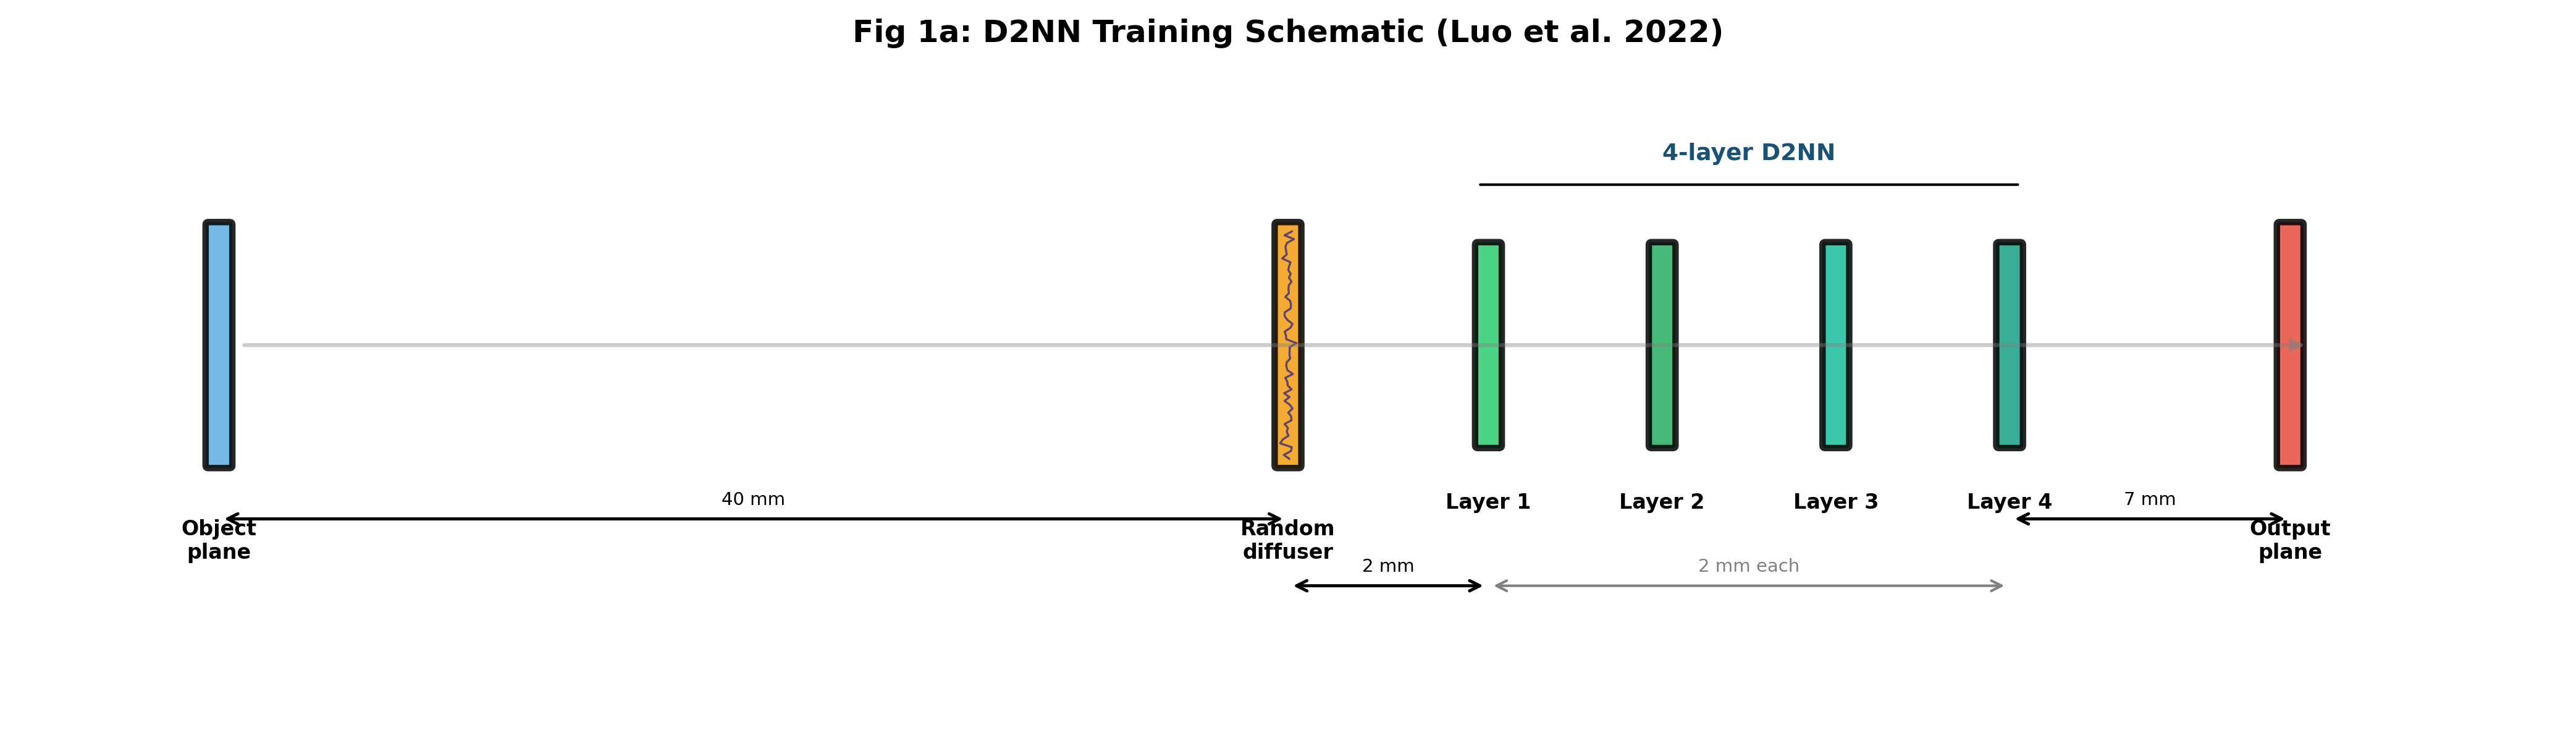
\includegraphics[width=0.95\textwidth]{fig1a_schematic.png}
  \caption{D2NN 시스템 개략도. 물체 평면에서 출발한 THz 파동이 랜덤 디퓨저를 통과한 뒤, 학습된 회절 레이어들을 거쳐 출력 평면에서 영상을 복원한다.}
  \label{fig:schematic}
\end{figure}

\begin{figure}[H]
  \centering
  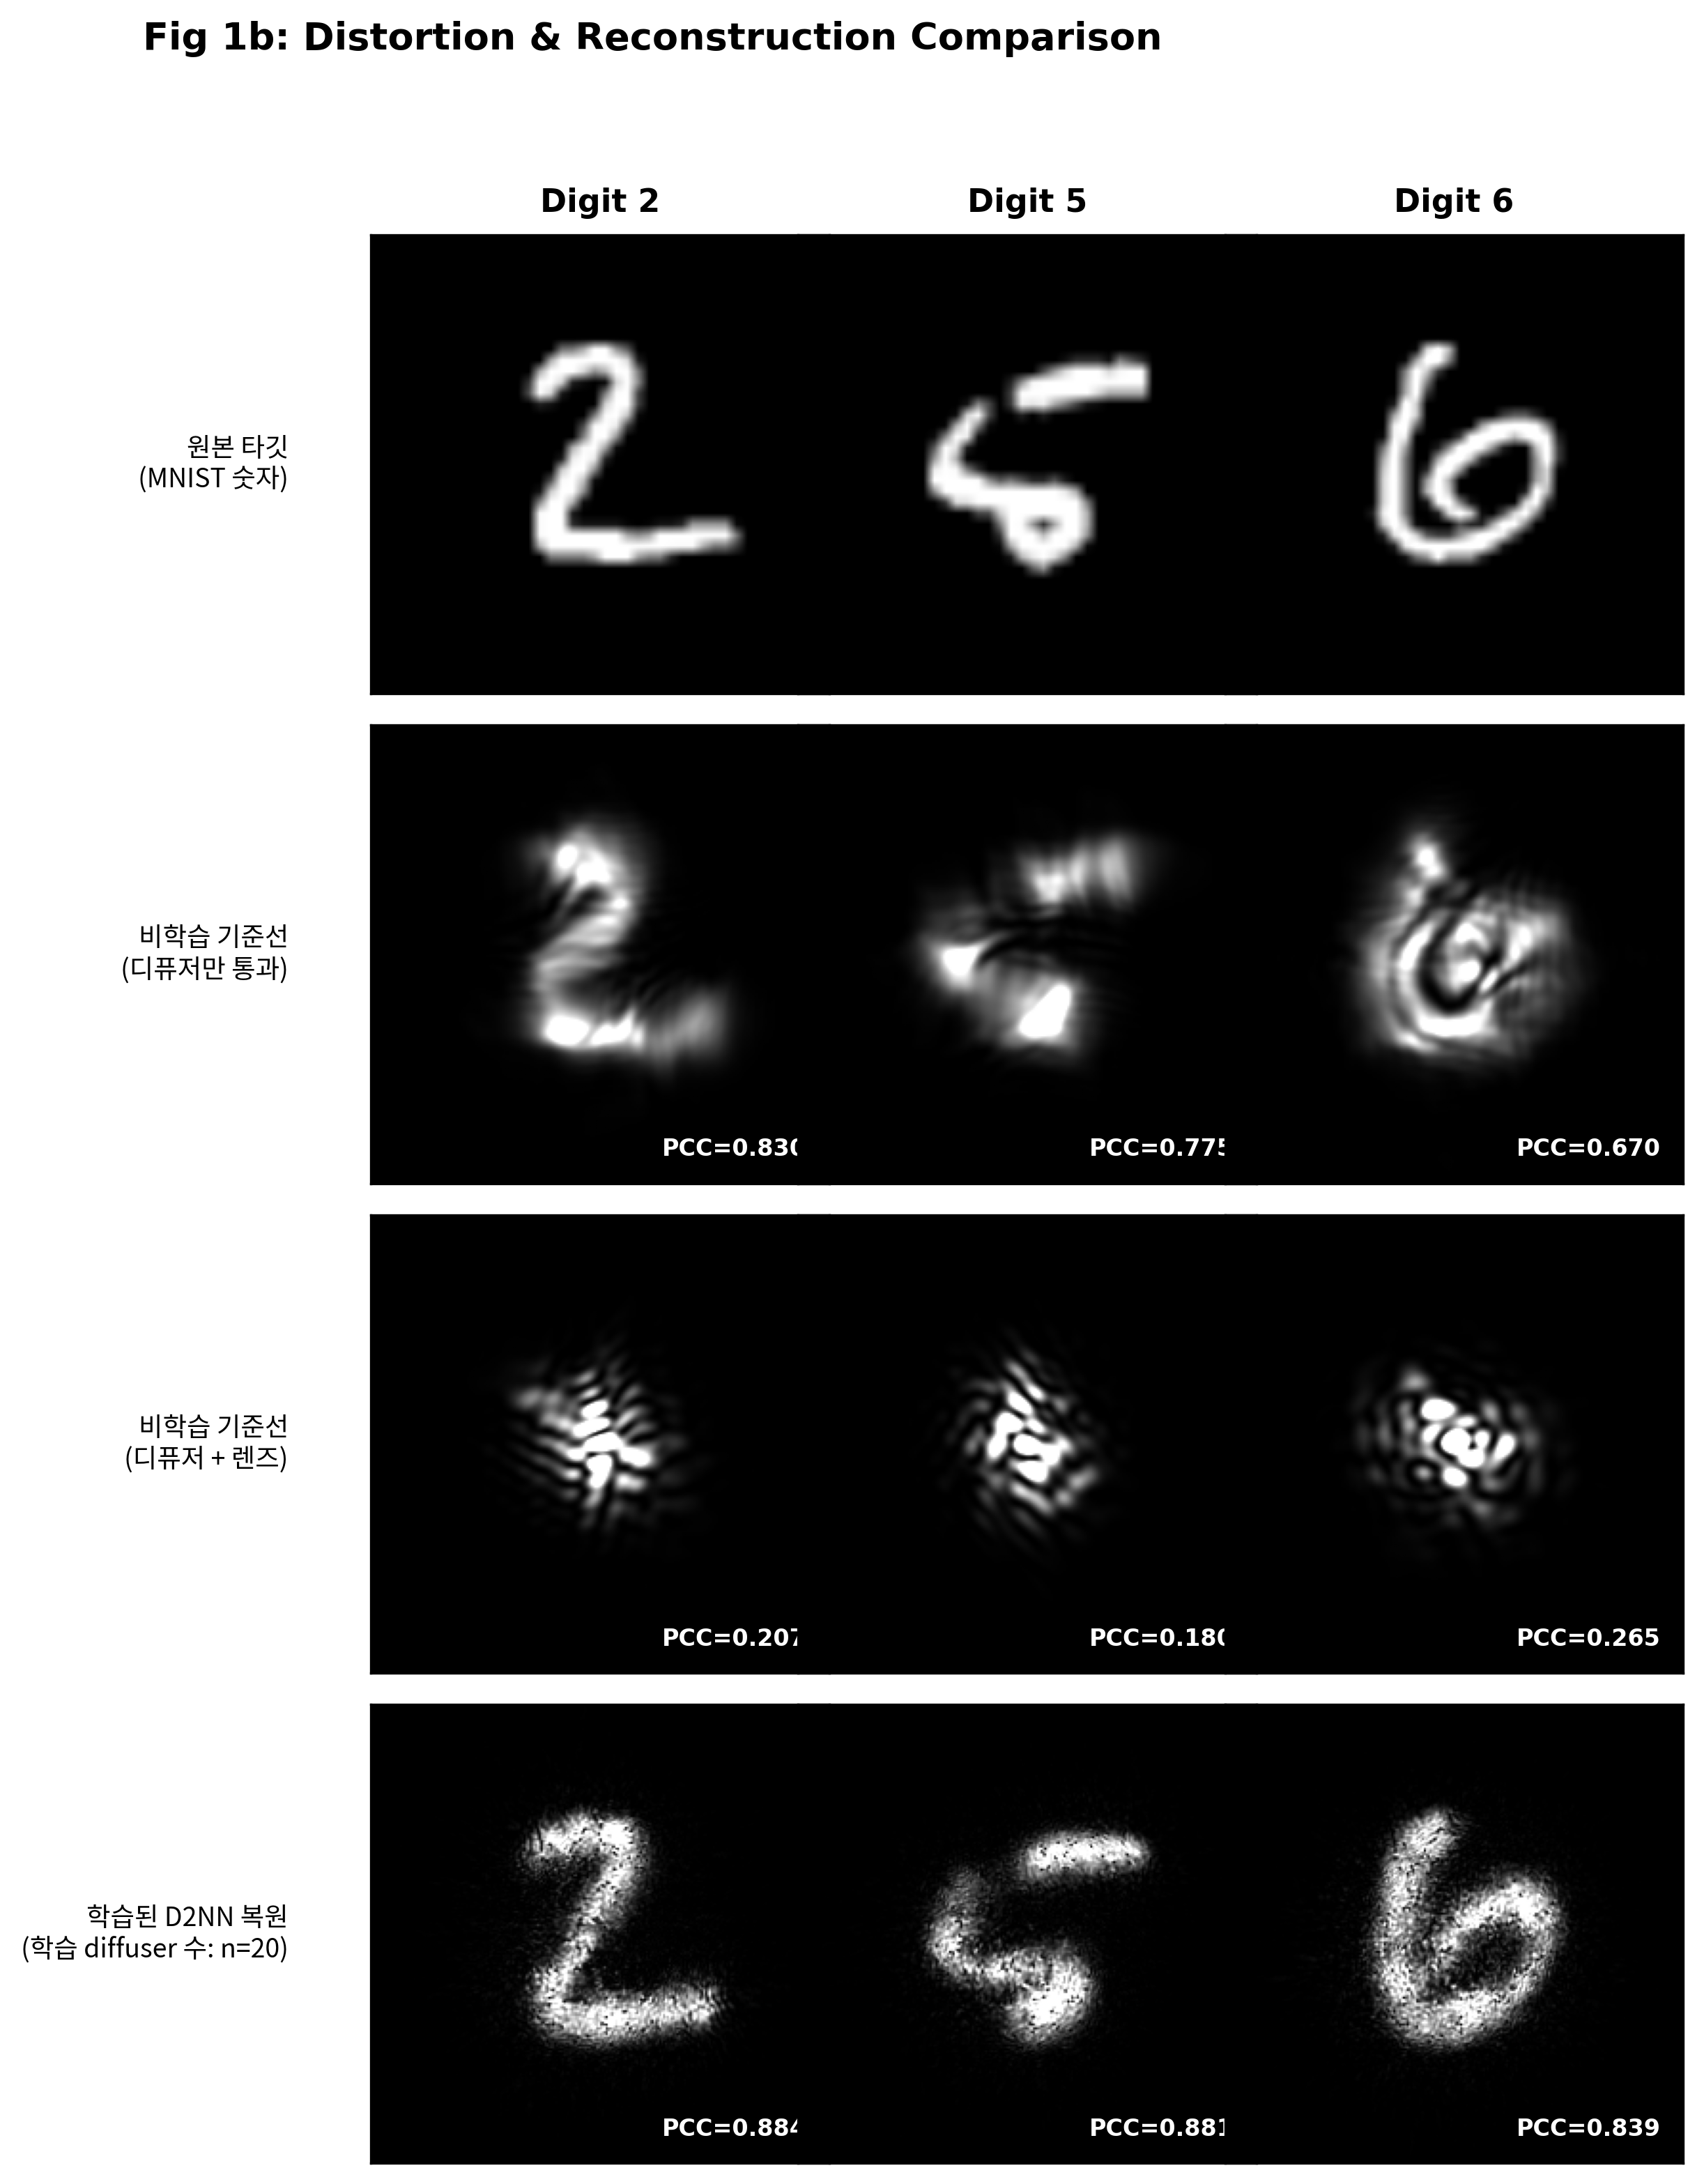
\includegraphics[width=0.85\textwidth]{fig1b_distortion.png}
  \caption{디퓨저에 의한 파면 왜곡(wavefront distortion) 효과. 입력 영상이 랜덤 위상 스크린을 통과하면 speckle 패턴으로 변환되며, D2NN은 이를 역전하여 원본을 복원한다.}
  \label{fig:distortion}
\end{figure}

\subsection{랜덤 디퓨저 접근법: Luo et al.\ 2022}

Luo 등의 2022년 연구\footnote{Y.\ Luo et al., ``Computational imaging without a computer: optical neural networks for imaging through random diffusers,'' \textit{eLight} \textbf{2}, 4 (2022).}는 이 한계를 정면으로 돌파한다. 핵심 아이디어는 다음과 같다:

\begin{insightbox}[핵심 아이디어]
학습 과정에서 매 에폭(epoch)마다 서로 다른 랜덤 디퓨저 $n$개를 삽입하여, D2NN이 특정 디퓨저의 역변환(inverse)을 암기하는 대신 \textbf{산란 통계(scattering statistics) 자체에 불변인 영상 복원 전략}을 학습하도록 유도한다.
\end{insightbox}

얇은 랜덤 위상 스크린(thin random phase screen)을 다음과 같이 모델링한다:
\begin{equation}\label{eq:diffuser}
  t_d(\mathbf{r}) = \exp\!\bigl[j\,\phi_d(\mathbf{r})\bigr],
  \qquad
  \phi_d = \frac{2\pi\,\Delta n\,D(\mathbf{r})}{\lambda}
\end{equation}
여기서 $D(\mathbf{r})$는 가우시안 평활화(Gaussian smoothing)를 거친 랜덤 높이맵(height map)이고, $\Delta n = 0.74$는 디퓨저 재료의 굴절률 차이이다.

\subsection{재현 프로젝트의 목적과 범위}

본 재현 프로젝트는 원논문의 핵심 결과를 독립적으로 검증하면서, 논문에 명시적으로 기술되지 않은 \textbf{암묵지(tacit knowledge)}를 체계적으로 발굴·문서화하는 것을 목표로 한다.

\begin{enumerate}
  \item \textbf{물리 시뮬레이션 엔진}: \blasm{} 기반 스칼라 회절 전파, $240 \times 240$ 그리드, $\Delta x = 0.3\;\text{mm}$, 400\,GHz
  \item \textbf{D2NN 모델}: 4-layer phase-only, $n = \{1, 10, 15, 20\}$ 스윕, 230,400 파라미터
  \item \textbf{Figure 재현}: Fig.~2 (known/new), Fig.~3 (grating period), Fig.~S1--S5
  \item \textbf{암묵지 발굴}: 상관길이, 위상 초기화, energy penalty, band-limiting 등 30개 항목
\end{enumerate}


% ============================================================
% SECTION 2 — 디퓨저 물리학
% ============================================================

\section{랜덤 위상 디퓨저의 물리학}\label{sec:diffuser}

\begin{insightbox}[Abstract]
랜덤 위상 디퓨저의 생성 원리, 가우시안 평활화와 상관길이의 수학적 관계($L = 2\sqrt{\pi}\,\sigma$), 그리고 디퓨저 다양성이 D2NN 성능에 미치는 영향을 분석한다. 특히 논문이 생략한 7가지 물리적 암묵지를 밝힌다.
\end{insightbox}

\subsection{생성 원리와 상관길이}

\subsubsection{코히런트 스칼라 모델의 필요충분성}

본 재현은 스칼라 회절 이론(scalar diffraction theory)에 기반한 코히런트 시뮬레이션을 채택한다. 동작 주파수 400\,GHz ($\lambda = 0.75\;\text{mm}$)에서 그리드 피치 $\Delta x = 0.3\;\text{mm}$는 $0.4\lambda$에 해당한다. 편광 효과가 유의미해지는 임계치($\Delta x \lesssim \lambda/2$)에 근접하지만, 디퓨저와 D2NN 레이어가 모두 \textbf{박막 위상 소자}(thin phase element)로 모델링되므로 스칼라 근사가 충분하다.

\begin{tkbox}[암묵지 --- 스칼라 모델의 선택]
스칼라 모델은 ``물리적으로 정확하기 때문에'' 쓰는 것이 아니라, 학습 가능한 수준의 계산 복잡도를 유지하면서도 논문의 핵심 메시지를 재현하기에 \textit{충분하기 때문에} 쓰는 것이다. Vector 모델로 전환하면 GPU 메모리가 $\sim$4배 증가한다.
\end{tkbox}

\subsubsection{디퓨저 높이맵 생성: 3단계 파이프라인}

디퓨저 생성 과정은 세 단계로 이루어진다 (Fig.~\ref{fig:diffuser_pipeline}):

\textbf{1단계 --- 백색 잡음 높이맵.}\quad
$W(x,y) \sim \mathcal{N}(\mu,\,\sigma_0^2)$, 여기서 $\mu = 25\lambda = 18.75\;\text{mm}$, $\sigma_0 = 8\lambda = 6.0\;\text{mm}$.

\begin{tkbox}[암묵지 --- 위상 wrapping과 균일 분포]
위상으로 변환하면 $\bar{\phi} = 2\pi \times 0.74 \times 25 \approx 116.2\;\text{rad} \approx 18.5 \times 2\pi$이고, $\sigma_\phi \approx 5.9 \times 2\pi$이다. 즉 위상이 $2\pi$를 여러 번 감싸므로, 투과 함수 $t_D = e^{j\phi_D}$의 위상은 사실상 $[0, 2\pi)$ \textbf{균일 분포}에 수렴한다. 이것이 논문의 ``uniform phase distribution''의 실체이다.
\end{tkbox}

\textbf{2단계 --- 가우시안 평활화.}\quad
$D(x,y) = (W * G_\sigma)(x,y)$, $\sigma = 4\lambda = 3.0\;\text{mm}$ (10\,px). 반사 패딩(reflect padding)과 분리 가능 필터링(separable filtering)을 사용한다.

\textbf{3단계 --- 위상 변환.}\quad
$t_D(x,y) = \exp\!\bigl(j\,2\pi\,\Delta n\,D(x,y)/\lambda\bigr)$, $\Delta n = 0.74$.

\begin{figure}[H]
  \centering
  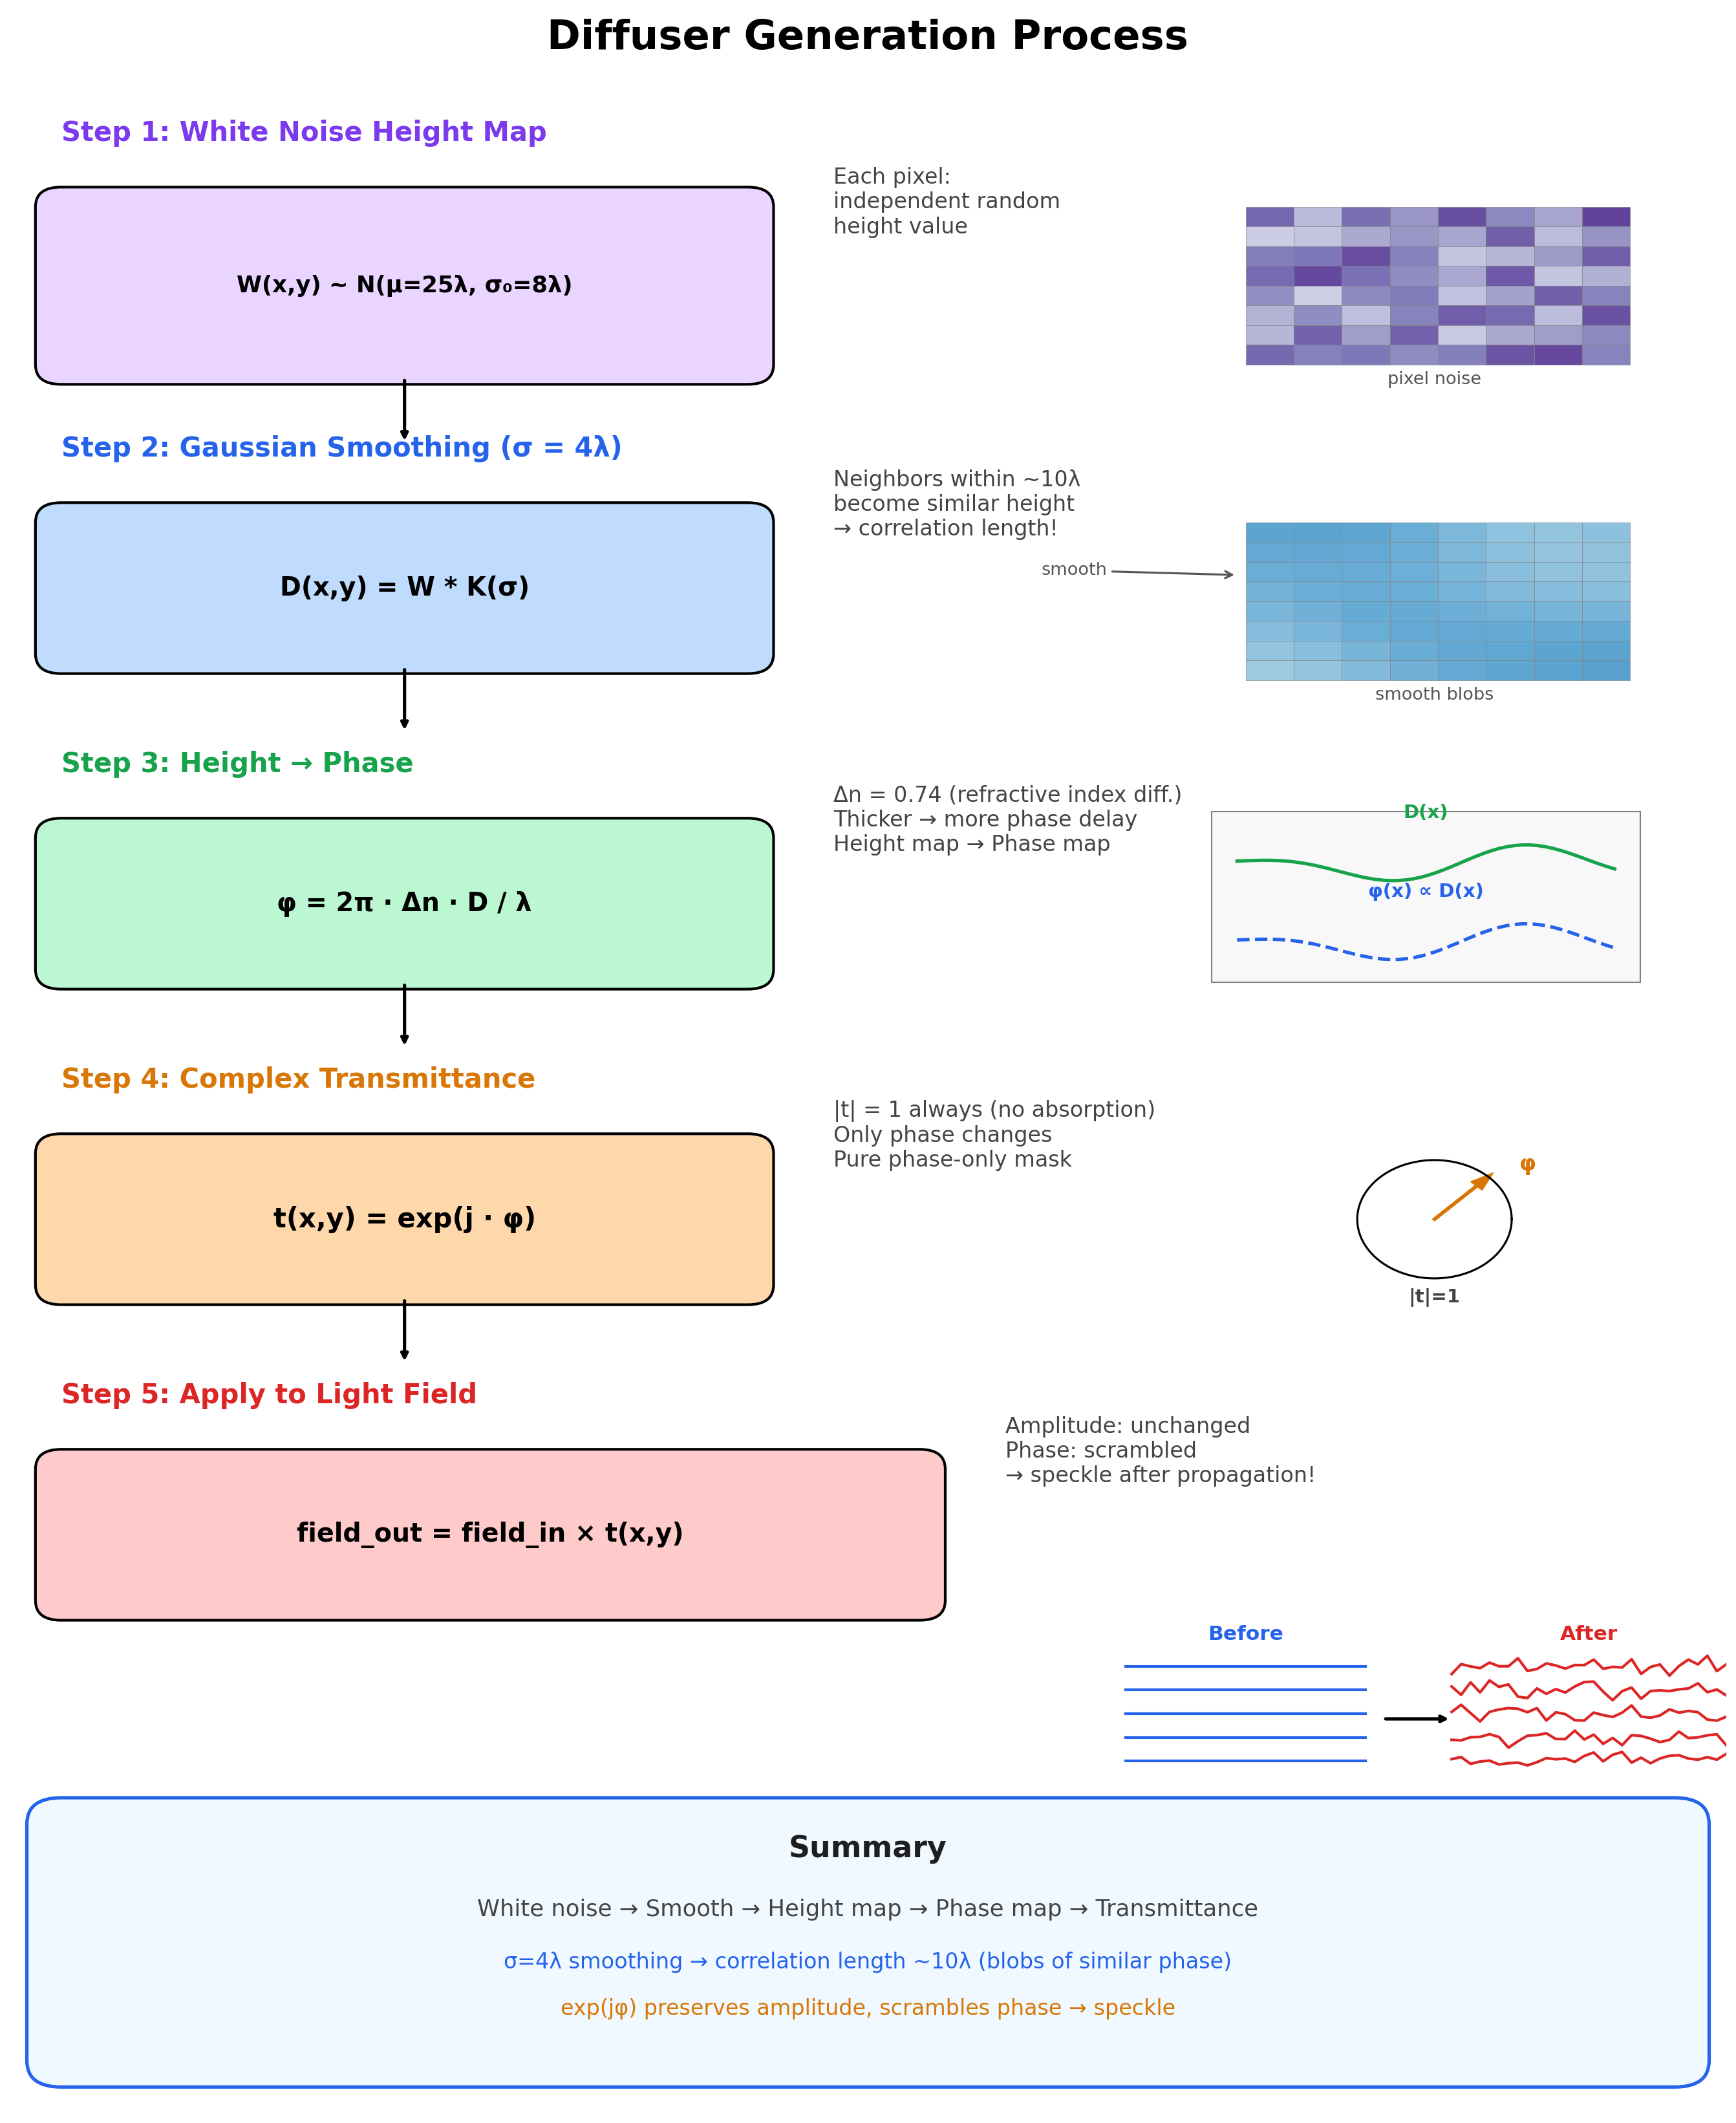
\includegraphics[width=0.75\textwidth]{diffuser_generation_diagram.png}
  \caption{디퓨저 생성 파이프라인의 3단계. 백색 잡음 높이맵에서 가우시안 평활화를 거쳐 위상 투과 함수로 변환된다.}
  \label{fig:diffuser_pipeline}
\end{figure}

\subsubsection{핵심 관계: 상관길이와 평활화 표준편차}

Wiener-Khinchin 정리에 의해, $D = W * G_\sigma$의 자기상관함수는:
\begin{equation}
  R_D(\mathbf{r}) \propto \exp\!\left(-\frac{|\mathbf{r}|^2}{4\sigma^2}\right)
\end{equation}

논문의 상관함수 정의 $R_d(\mathbf{r}) = \exp(-\pi|\mathbf{r}|^2/L^2)$와 비교하면:
\begin{equation}\label{eq:corr_length}
  \boxed{L = 2\sqrt{\pi}\,\sigma}
\end{equation}

기본 설정 $\sigma = 4\lambda$에서 이론적 $L = 14.18\lambda$이고, 실제 측정값은 $L \approx 16.09\lambda$이다 (이산화 및 경계 효과).

\begin{figure}[H]
  \centering
  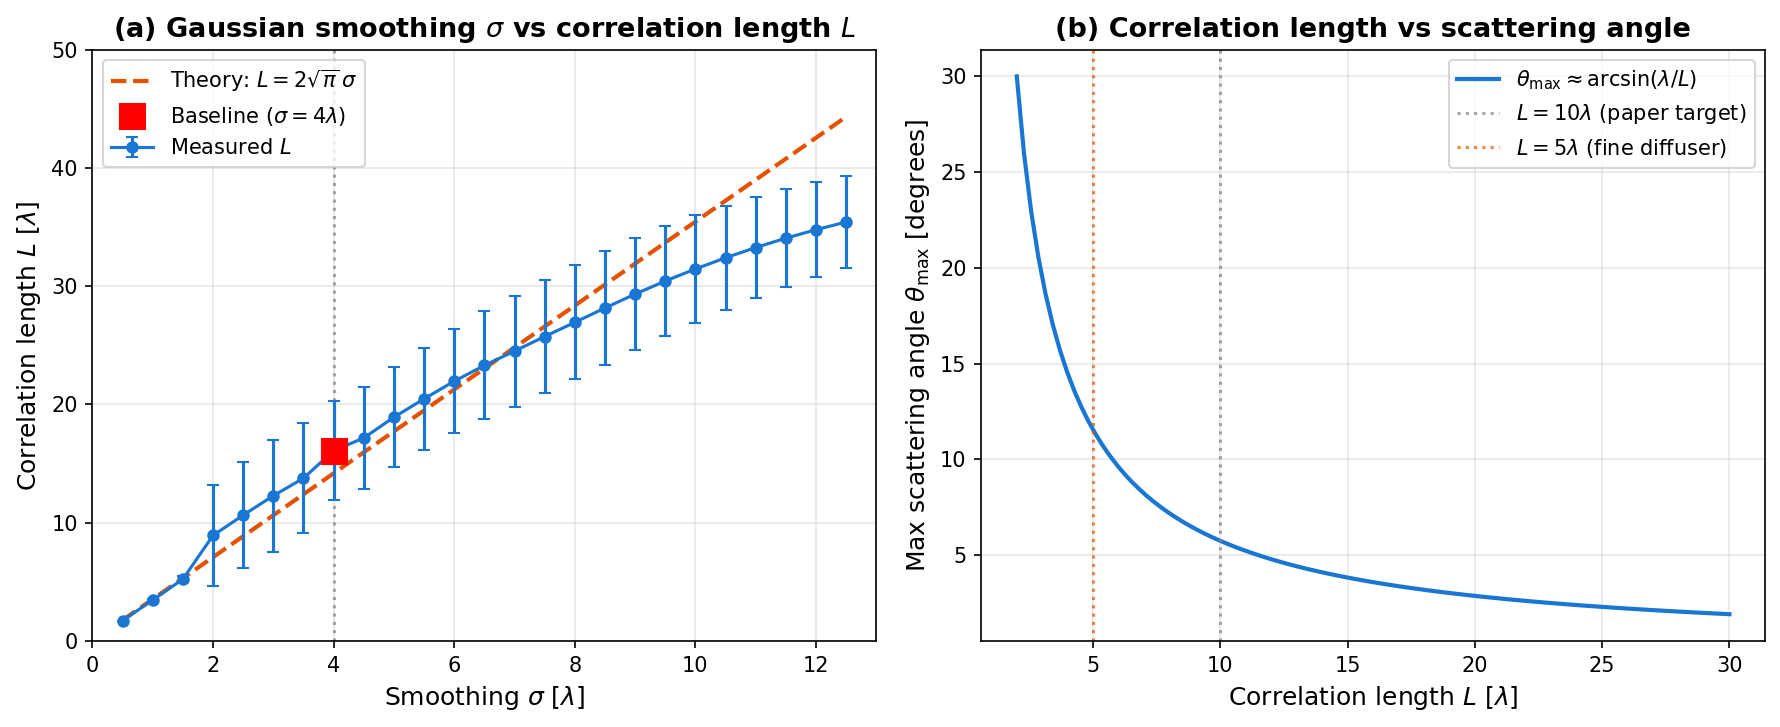
\includegraphics[width=0.85\textwidth]{fig_correlation_physics.png}
  \caption{(a) 평활화 표준편차 $\sigma$와 측정된 상관길이 $L$의 관계. 이론 곡선 $L = 2\sqrt{\pi}\sigma$와 비교. (b) 상관길이에 따른 최대 산란각.}
  \label{fig:correlation}
\end{figure}

\subsubsection{패딩 팩터 = 2의 물리적 의미}

\blasm{} 전파에서 \texttt{pad\_factor: 2}는 $N \times N$ 필드를 $2N \times 2N$으로 제로 패딩한다. 길이 $N$인 두 신호의 선형 합성곱 결과 길이는 $2N-1$이므로, $2N = 480 \geq 479$는 \textbf{정확히 최소 요구치}를 충족한다.

\subsubsection{소멸파 차단}

\blasm{} 전달 함수에서 소멸파(evanescent wave)를 strict inequality로 마스킹한다:
\begin{equation}
  H(f_x, f_y;\,z) = \begin{cases}
    \exp\!\left(j\,2\pi z\sqrt{1/\lambda^2 - f_x^2 - f_y^2}\right), & f_x^2 + f_y^2 < 1/\lambda^2 \\
    0, & \text{otherwise}
  \end{cases}
\end{equation}

격자의 공간 주파수 범위 중 약 \textbf{36\%}가 소멸파로 차단된다. 이는 물리적으로 전파 불가능한 성분을 정확히 제거하는 것이다.

\subsubsection{uniqueness\_delta\_phi의 의미}

서로 다른 디퓨저 인스턴스 간의 최소 위상 차이 기준이다. $e^{j0}$과 $e^{j\pi/2} = j$는 복소 평면에서 직교하므로, 이 값은 디퓨저 다양성의 하한을 보장하는 \textbf{직교성 조건}(orthogonality condition)이다.

\subsection{디퓨저 다양성이 광학장에 미치는 영향}

\subsubsection{상관길이와 산란각}

산란각은 $\theta_\text{max} \approx \arcsin(\lambda/L)$로 결정된다. $L = 10\lambda$이면 $\theta_\text{max} \approx 5.7°$이다.

\begin{table}[H]
\centering
\caption{Fig.~S5 재현: 상관길이에 따른 PCC 변화. $L \sim 10\lambda$에서 학습된 모델이 $L \sim 5\lambda$를 만나면 성능이 급락한다.}
\label{tab:corr_pcc}
\begin{tabular}{l c c c}
\toprule
\thead{모델} & \thead{Known\\($L \sim 10\lambda$)} & \thead{New\\($L \sim 10\lambda$)} & \thead{New\\($L \sim 5\lambda$)} \\
\midrule
$n = 1$  & 0.761 & 0.769 & 0.496 \\
$n = 10$ & 0.835 & 0.854 & 0.609 \\
$n = 15$ & 0.830 & 0.850 & 0.586 \\
$n = 20$ & 0.846 & 0.860 & 0.635 \\
\bottomrule
\end{tabular}
\end{table}

\begin{figure}[H]
  \centering
  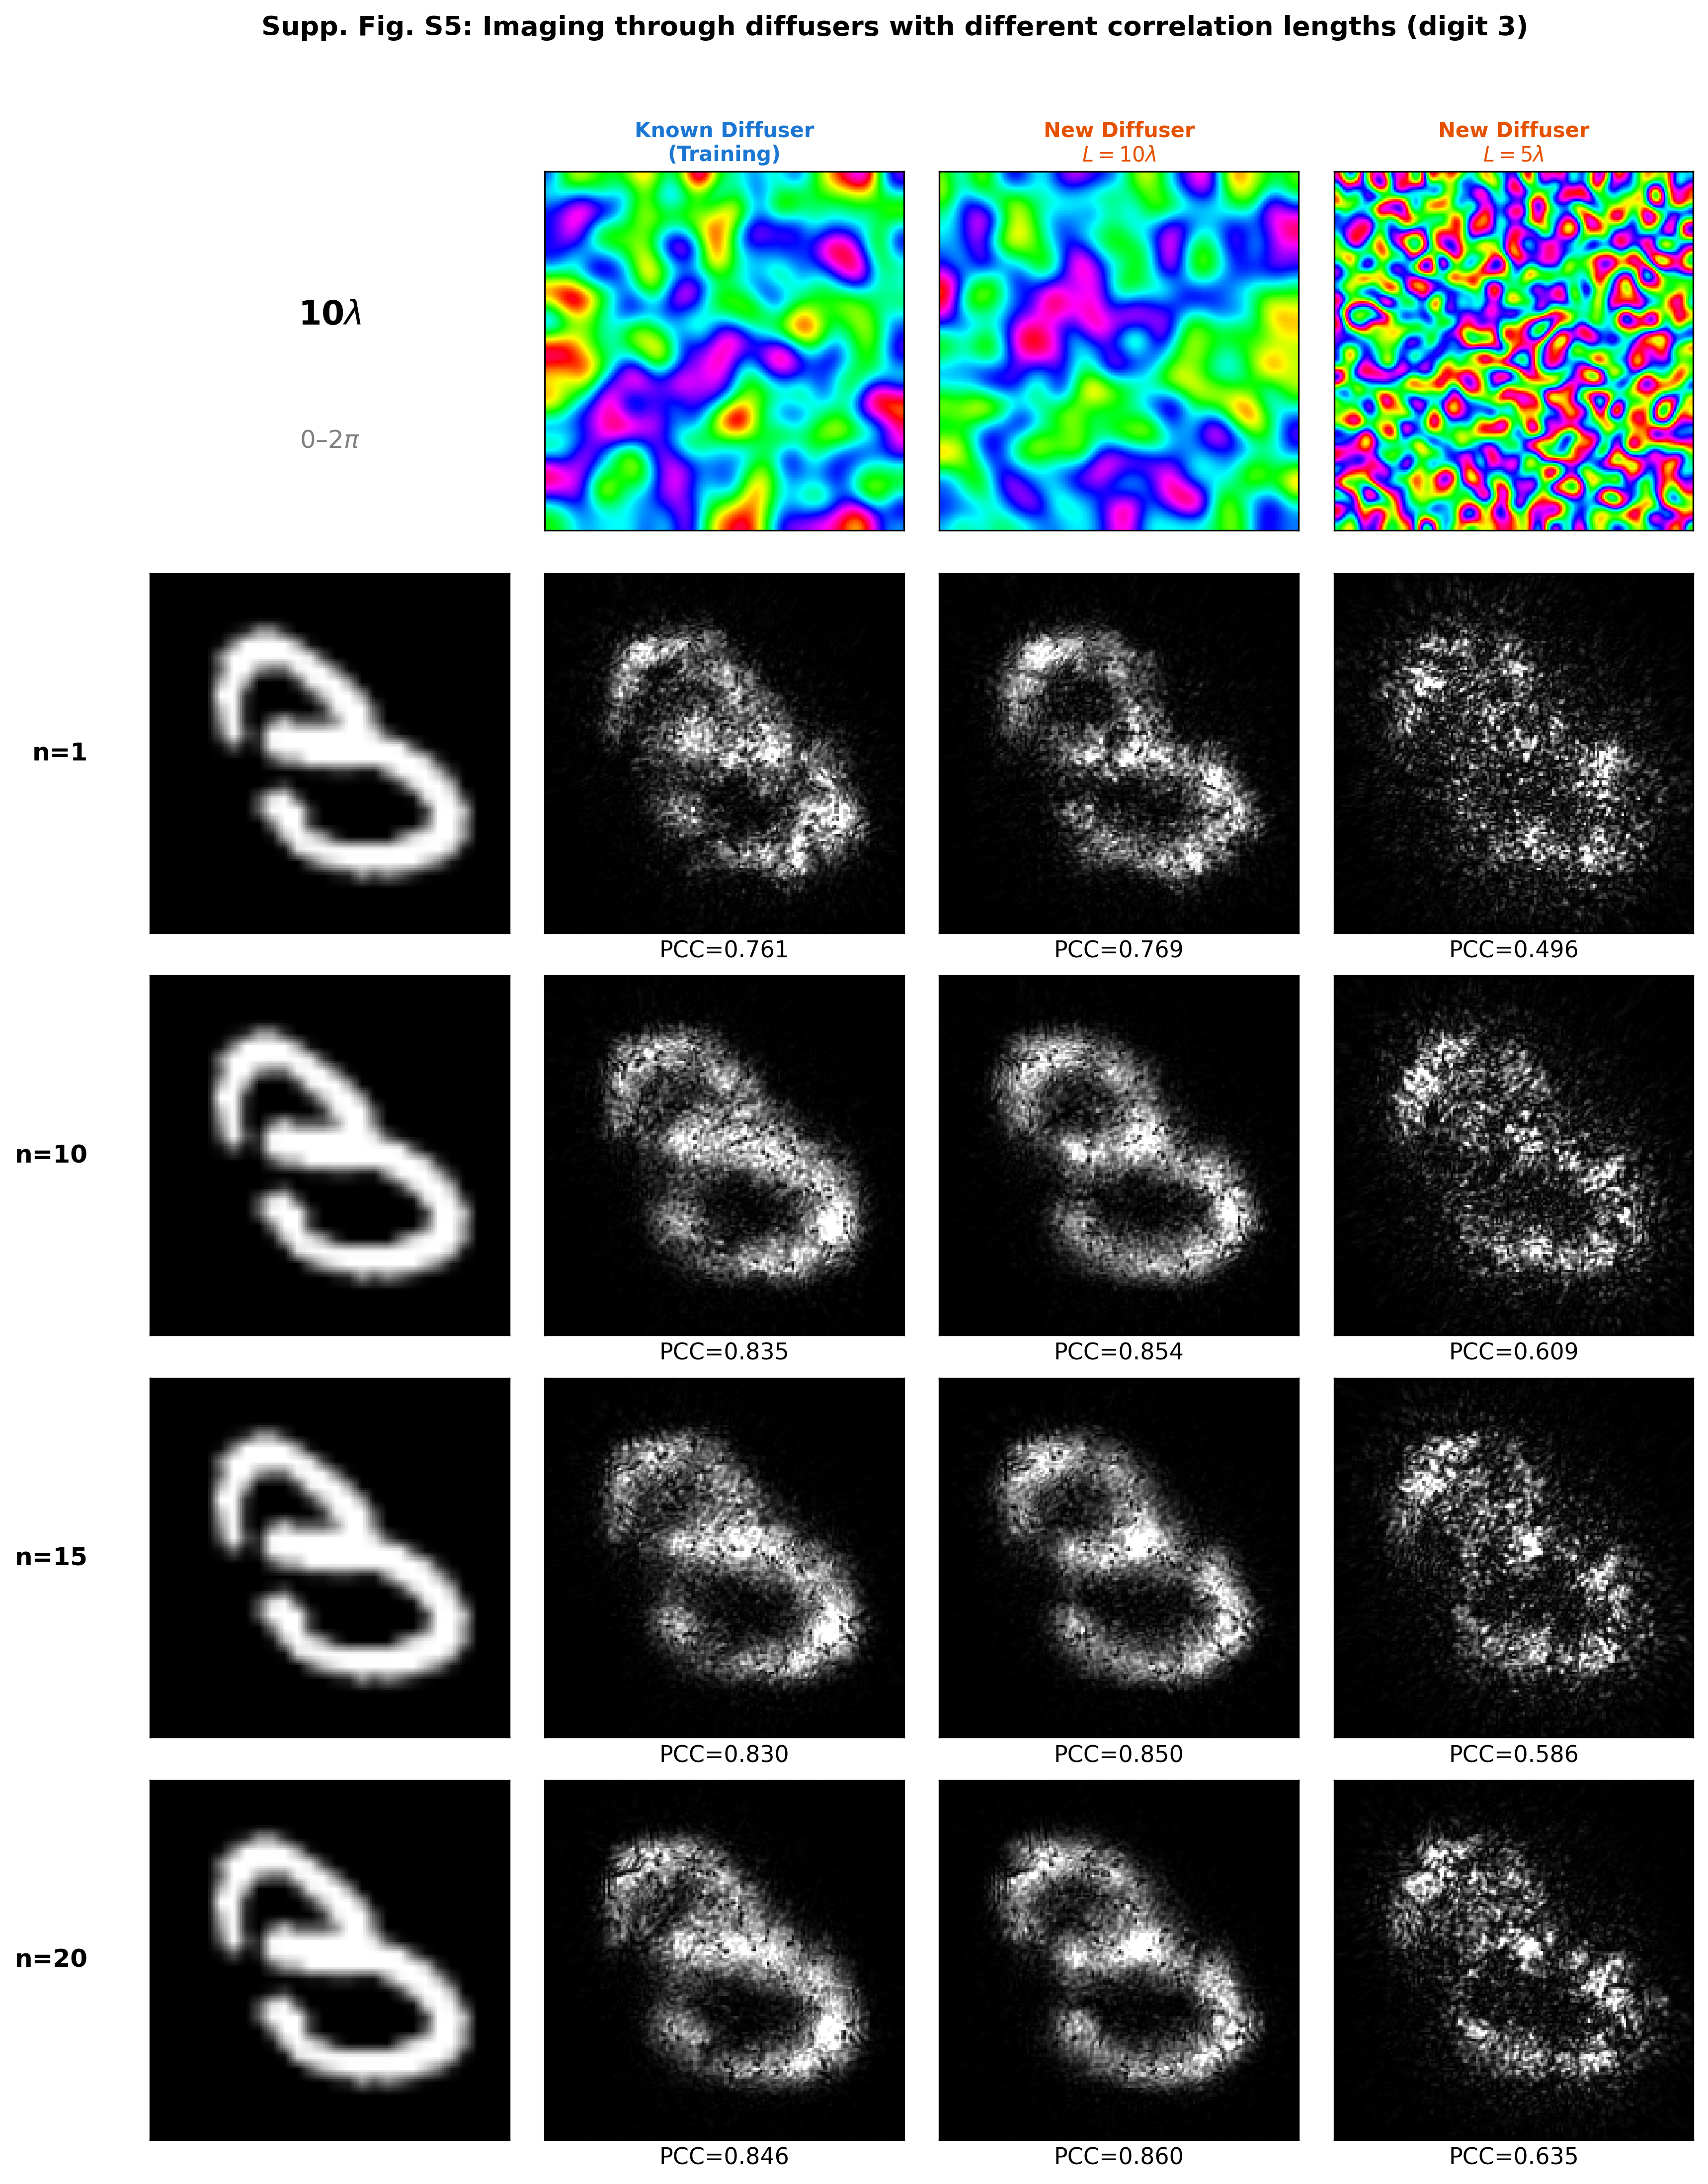
\includegraphics[width=0.85\textwidth]{figS5_corr_length.png}
  \caption{\textbf{Fig.~S5 재현}: 상관길이가 다른 디퓨저에 대한 D2NN 성능 비교. $L \sim 10\lambda$로 학습된 모델이 $L \sim 5\lambda$ 디퓨저를 만나면 PCC가 급격히 하락한다.}
  \label{fig:figS5}
\end{figure}

\subsubsection{인스턴스 다양성 vs 통계적 다양성}

D2NN은 \textbf{인스턴스 다양성}(동일 통계, 다른 시드)에는 강건하지만, \textbf{통계적 다양성}(다른 $L$)에는 취약하다. 이는 학습된 역변환이 특정 산란각 분포에 특화되어 있기 때문이다.

\begin{tkbox}[암묵지 --- 역문제의 풀 수 있는 조건]
디퓨저의 산란 대역폭 $f_\text{diff} \sim 1/L = 0.133\;\text{mm}^{-1}$은 물체의 유효 대역폭 $\sim 0.89\;\text{mm}^{-1}$보다 훨씬 좁다. 이 조건 --- $f_\text{diff} \ll f_\text{object}$ --- 이 D2NN이 역문제를 풀 수 있는 물리적 근거이다.
\end{tkbox}


\begin{figure}[H]
  \centering
  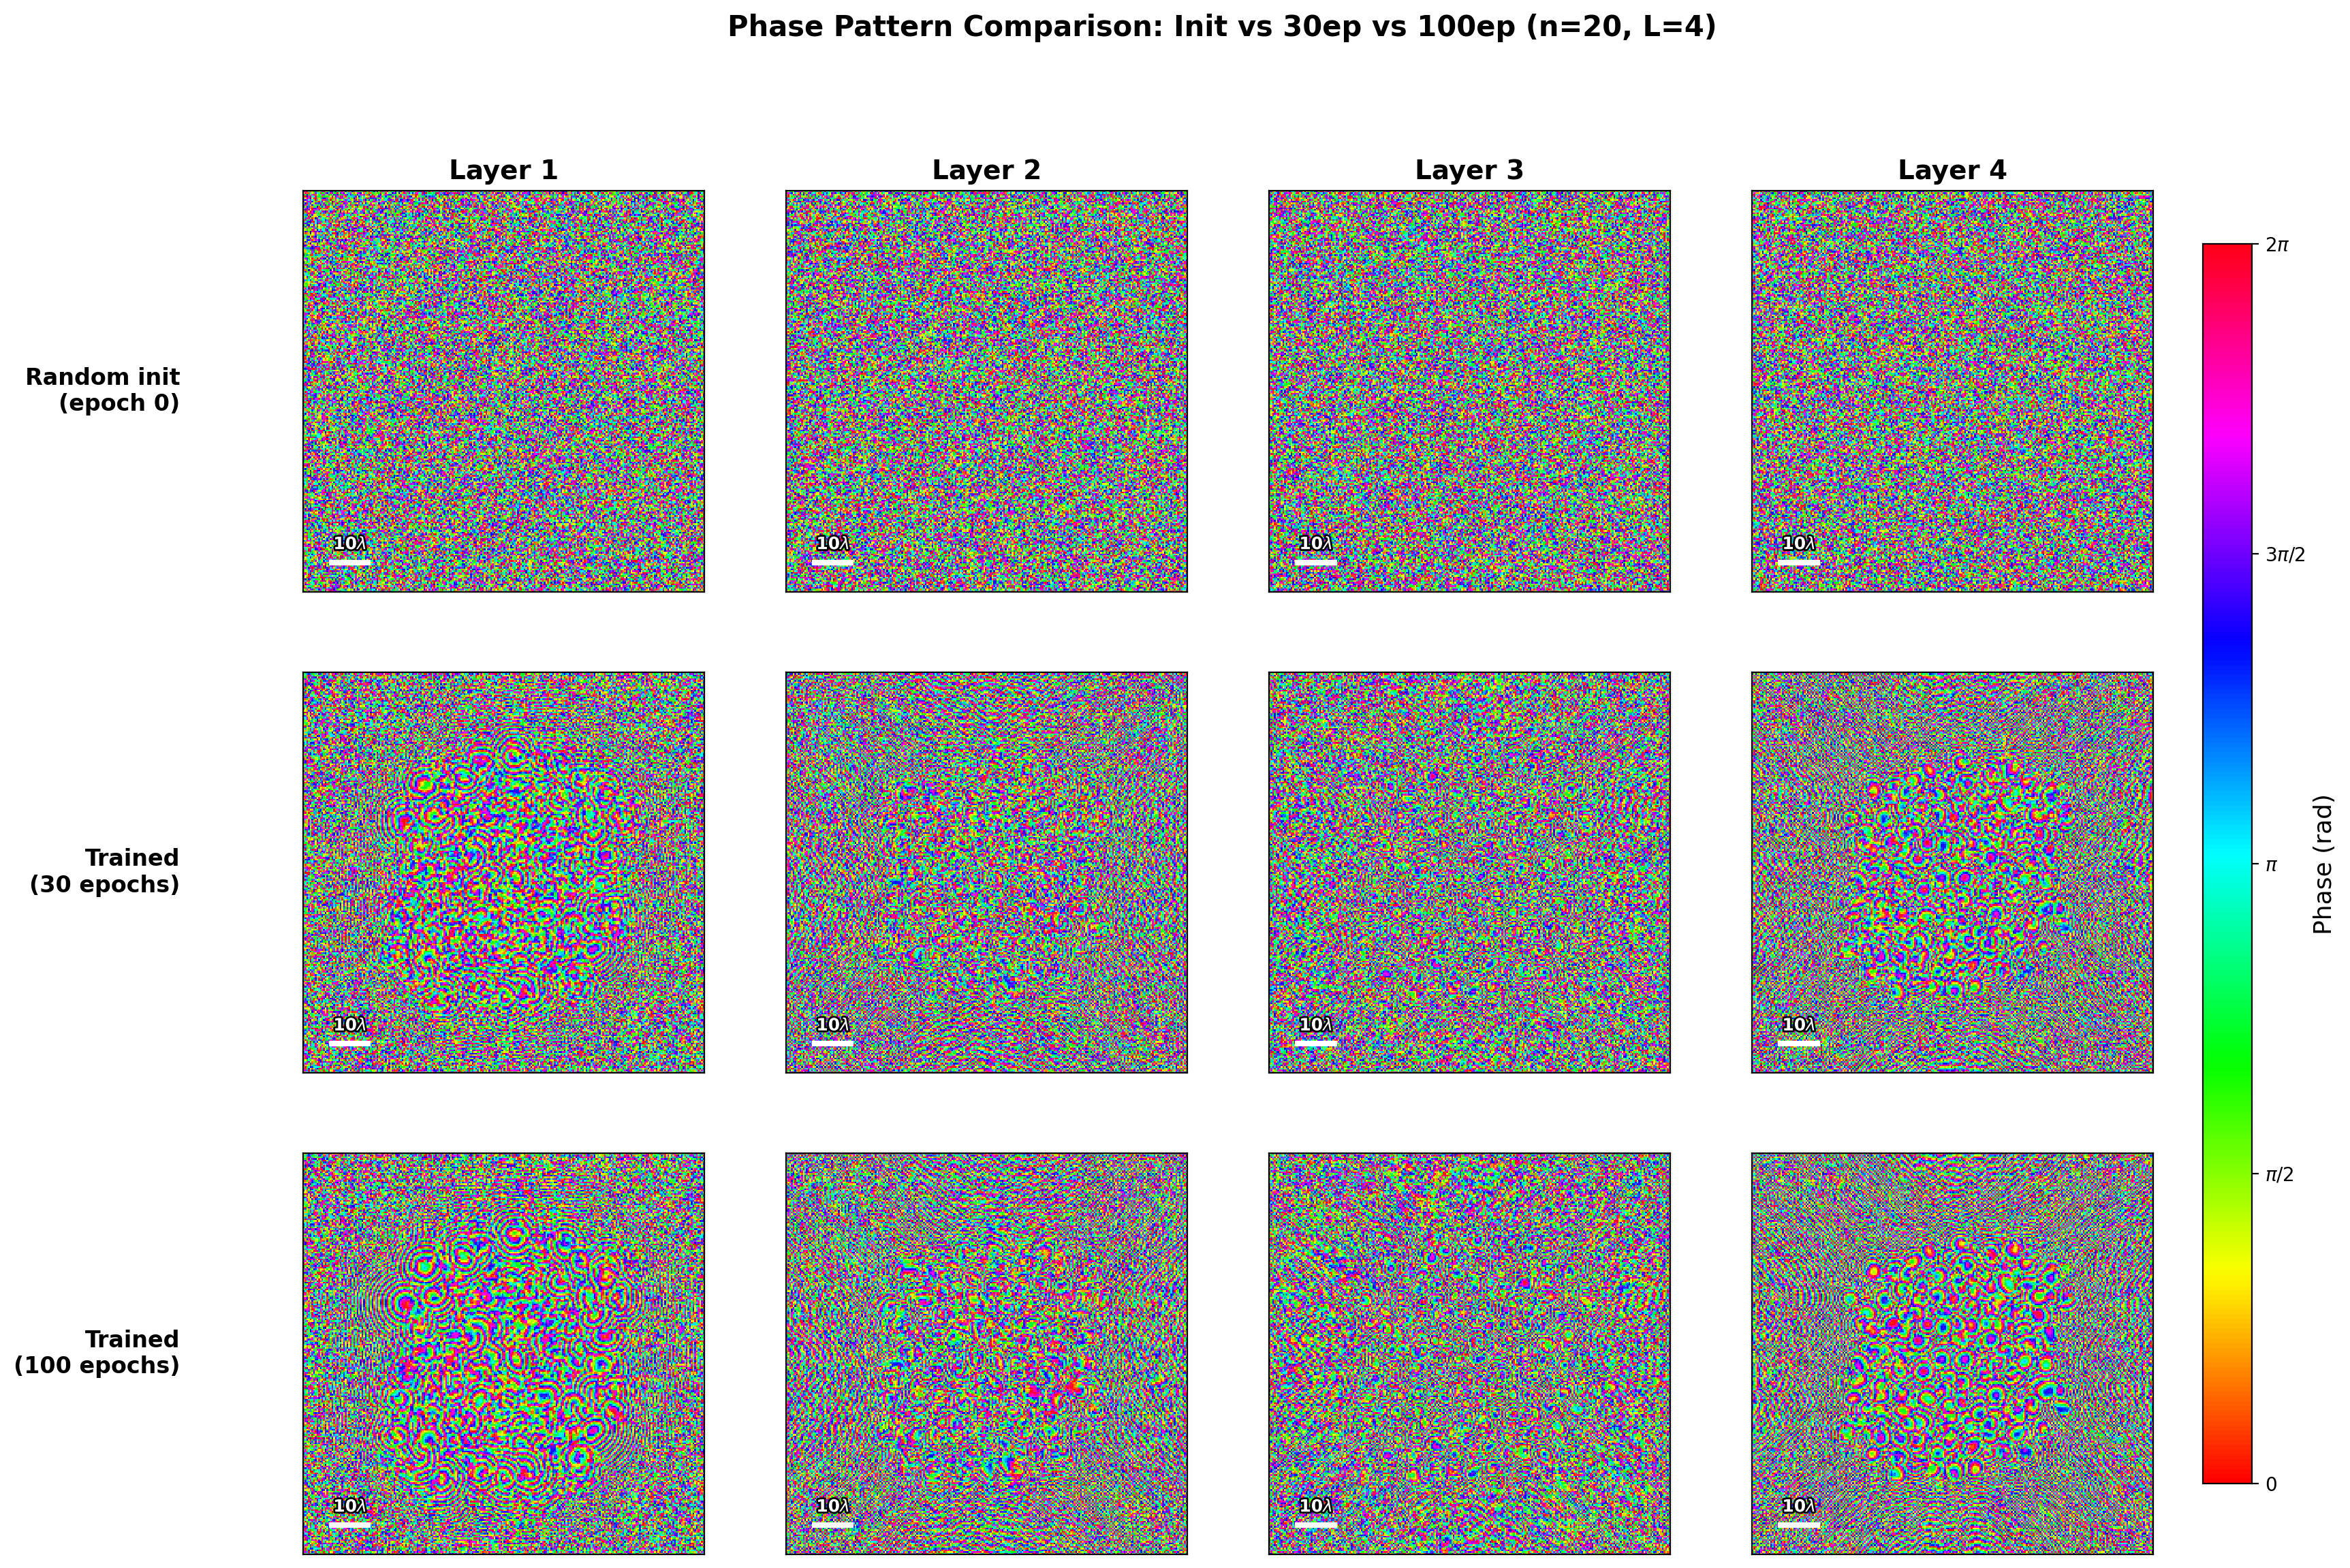
\includegraphics[width=0.85\textwidth]{figS1_phase_comparison.png}
  \caption{\textbf{Fig.~S1a 재현}: 학습 전후의 위상 레이어 비교. 학습 전 위상은 $[0, 2\pi)$ 균일 분포이며, 학습 후에는 특정 영역에 위상이 집중되는 ``위상 섬(phase island)'' 구조가 형성된다. 이 구조는 D2NN이 산란 보정을 위해 특정 공간주파수 채널을 선택적으로 활용함을 보여준다.}
  \label{fig:figS1a}
\end{figure}

\begin{figure}[H]
  \centering
  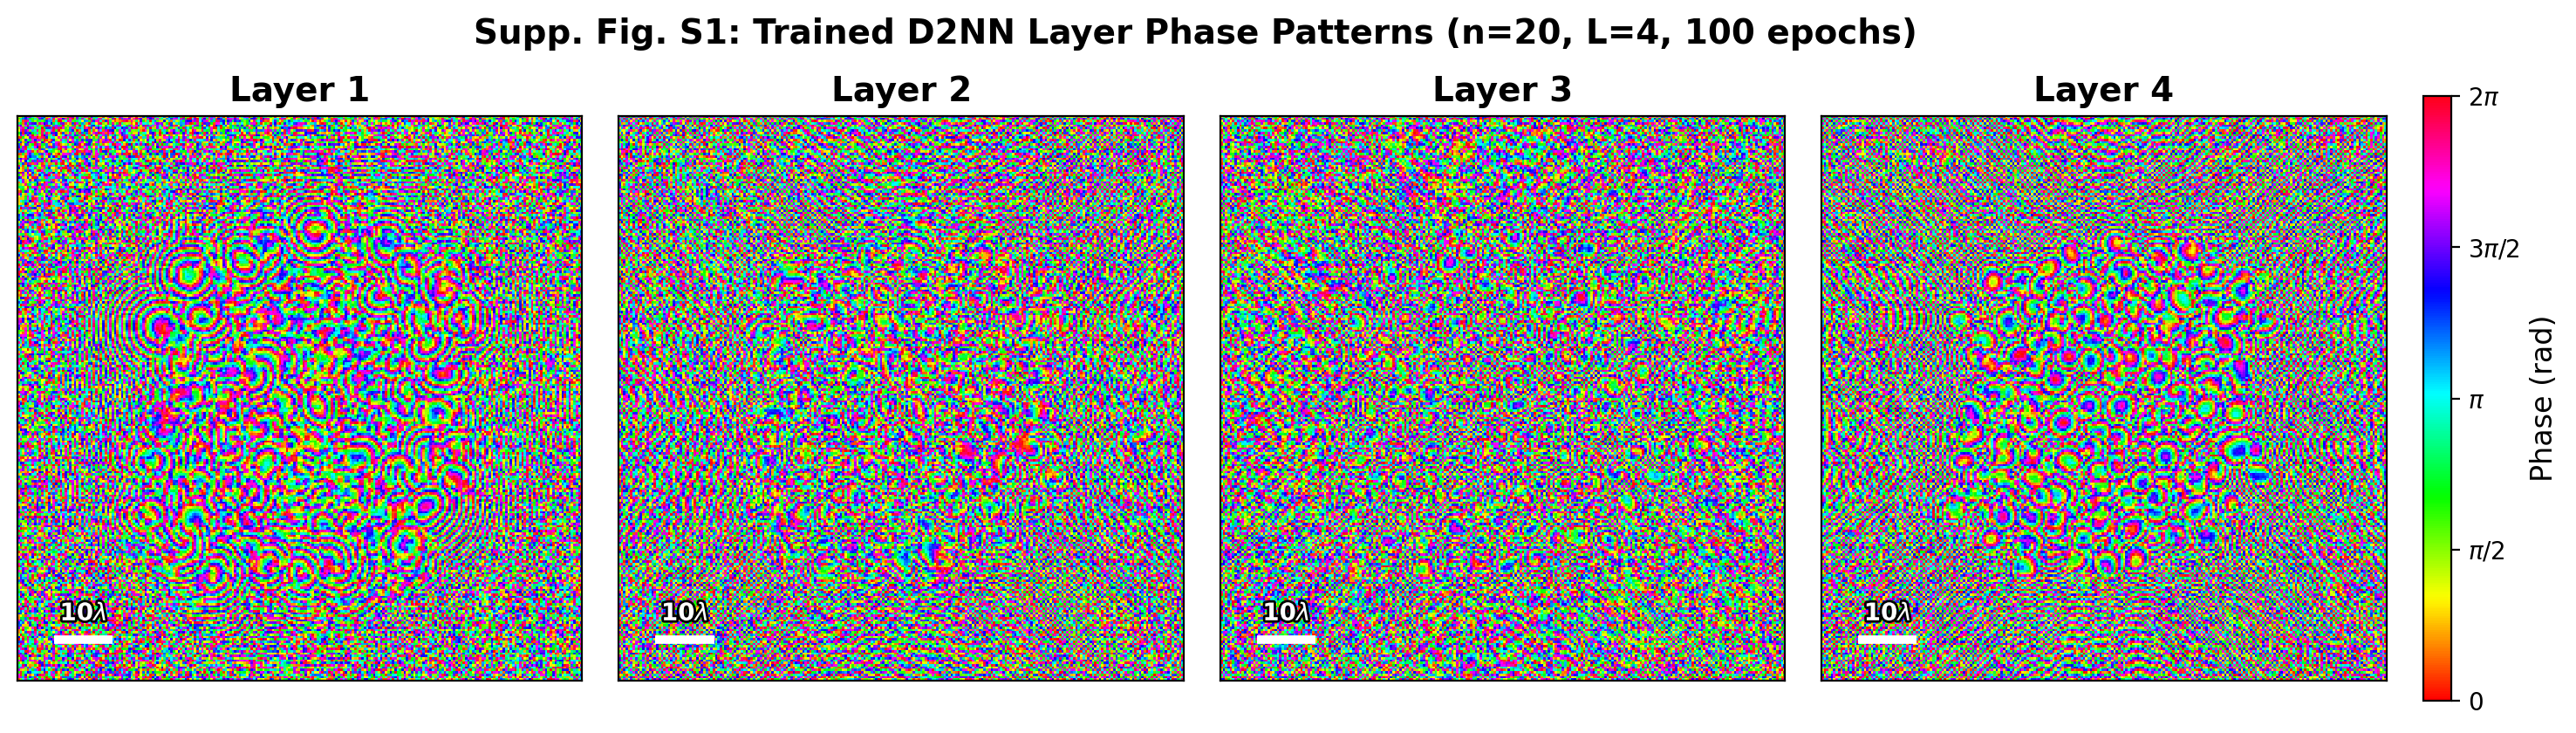
\includegraphics[width=0.95\textwidth]{figS1_layer_phases.png}
  \caption{\textbf{Fig.~S1b 재현}: 4개 레이어 각각의 학습된 위상 패턴. Layer~1은 디퓨저에 가장 가까워 입력 산란을 초기 보정하며 비교적 부드러운 패턴을 보인다. Layer~4는 출력에 가까워 세밀한 위상 조절로 최종 intensity 패턴을 형성한다. 레이어 깊이에 따른 위상 복잡도의 증가는 D2NN이 점진적 정보 처리(progressive information processing)를 수행함을 시사한다.}
  \label{fig:figS1b}
\end{figure}

% ============================================================
% SECTION 3 — 시스템 설계
% ============================================================

\section{D2NN 시스템 설계의 해부}\label{sec:system}

\begin{insightbox}[Abstract]
240$\times$240 그리드, 0.3\,mm 피치, 4-layer D2NN의 모든 설계 파라미터가 왜 그 값이어야 하는지를 \blasm{} 전파 물리에 근거하여 해부한다. 핵심 발견: 이 파라미터 세트는 개별 최적값의 모음이 아니라, \textbf{상호 의존적 제약을 동시에 만족하는 하나의 일관된 설계점}이다.
\end{insightbox}

\begin{figure}[H]
  \centering
  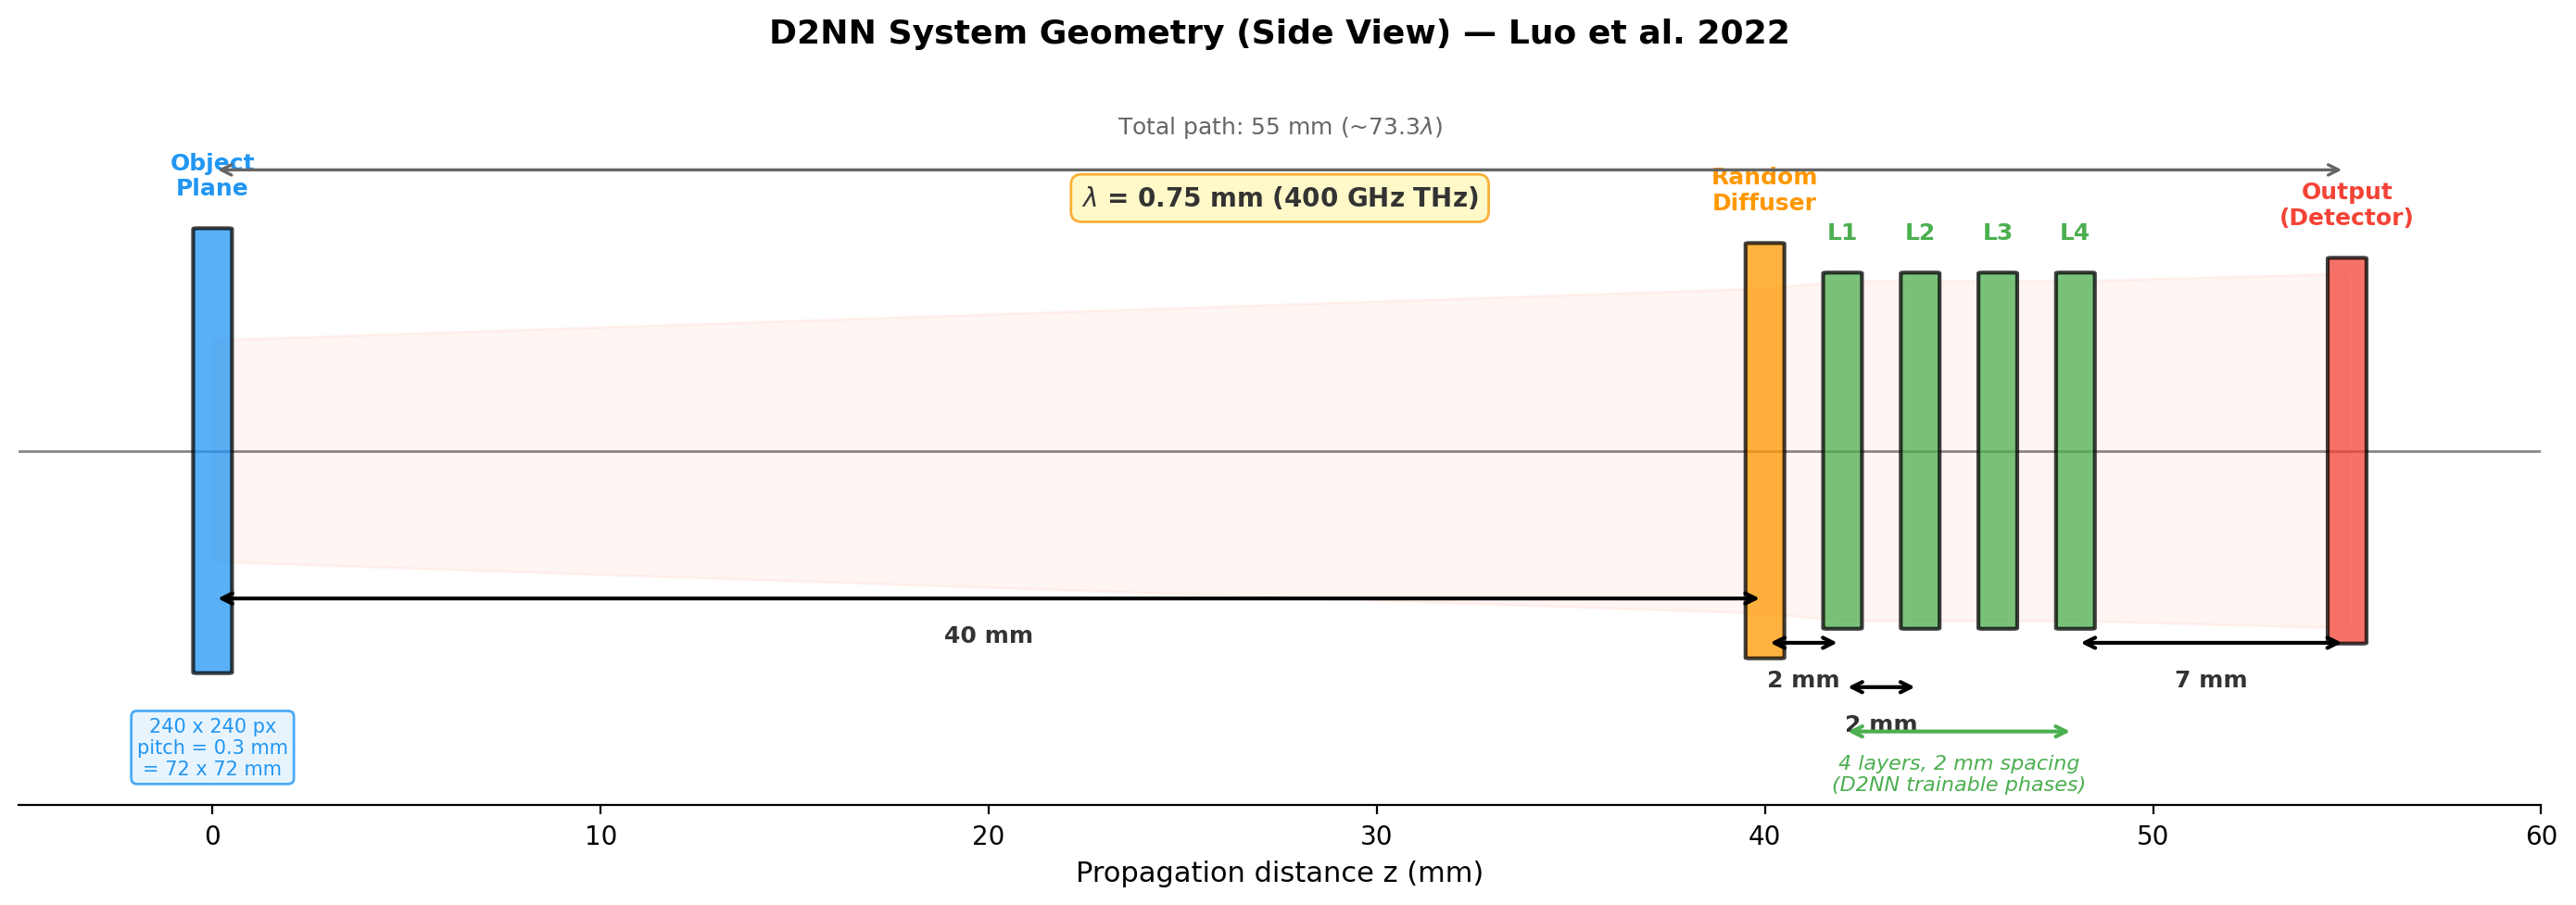
\includegraphics[width=0.95\textwidth]{fig_system_geometry.png}
  \caption{D2NN 광학 시스템의 측면 기하 배치. Object plane에서 random diffuser를 거쳐 4개의 학습 가능한 phase layer를 통과한 뒤 output detector plane에 도달한다.}
  \label{fig:geometry}
\end{figure}

\subsection{BL-ASM 전파와 설계 제약}

\subsubsection{Nyquist 제약과 피치 선택}

Shannon-Nyquist 정리에 의해 전파 가능 최대 공간 주파수 $f_\text{max} = 1/\lambda$를 표현하려면:
\begin{equation}
  \Delta x \leq \frac{\lambda}{2} = 0.375\;\text{mm}
\end{equation}

\begin{tkbox}[암묵지 1 --- 피치 = 0.3\,mm]
$\Delta x = 0.3\;\text{mm}$는 Nyquist 한계의 80\%로, ``적당히 고른 값''이 아니라 계산 효율과 물리적 정확성을 절충한 \textbf{최적점}이다. $\Delta x > 0.375$이면 aliasing, 불필요하게 작으면 $O(N^2 \log N)$ 계산량 급증.
\end{tkbox}

유효 수치 개구수 $\text{NA}_\text{eff} = \lambda \cdot f_\text{max} = 1.0$이며, 이론적 최대 해상도는:
\begin{equation}
  \delta_\text{min} = \frac{\lambda}{2\,\text{NA}_\text{eff}} = 0.375\;\text{mm}
\end{equation}
\textbf{해상도 한계는 그리드 샘플링이 아니라 파동 물리에 의해 결정된다.}

\subsection{기하학적 배치의 물리적 의미}

\begin{table}[H]
\centering
\caption{D2NN 전체 광학 경로. 각 구간의 거리와 Fresnel 확산 폭.}
\label{tab:path}
\begin{tabular}{l r r r}
\toprule
\thead{구간} & \thead{거리 (mm)} & \thead{$z/\lambda$} & \thead{Fresnel 확산 (px)} \\
\midrule
Object $\to$ Diffuser       & 40.0 & 53.3 & ---   \\
Diffuser $\to$ Layer\,1     &  2.0 &  2.67 & 4.1  \\
Layer\,1 $\to$ Layer\,2     &  2.0 &  2.67 & 4.1  \\
Layer\,2 $\to$ Layer\,3     &  2.0 &  2.67 & 4.1  \\
Layer\,3 $\to$ Layer\,4     &  2.0 &  2.67 & 4.1  \\
Layer\,4 $\to$ Output       &  7.0 &  9.33 & 7.6  \\
\midrule
\textbf{합계}               & \textbf{55.0} & \textbf{73.3} & --- \\
\bottomrule
\end{tabular}
\end{table}

\begin{tkbox}[암묵지 2 --- Object-to-Diffuser 40\,mm]
Fresnel number $F = a^2/(\lambda z) = 24^2/(0.75 \times 40) = 19.2$. ``물체 정보가 diffuser 전면에 충분히 퍼지되, 패딩 영역을 넘어가지 않는'' 절충점이다.
\end{tkbox}

\begin{tkbox}[암묵지 3 --- Layer 간격 2\,mm $\Rightarrow$ 광학적 receptive field]
단일 픽셀의 Fresnel 확산 폭 $w = \sqrt{\lambda z} = \sqrt{0.75 \times 2} = 1.225\;\text{mm} \approx 4.1\;\text{pixels}$. 이것이 D2NN의 ``receptive field''를 결정하며, CNN의 3$\times$3/5$\times$5 커널에 대응한다. 4개 layer를 거치면 누적 receptive field $\approx 16$\,pixels로, MNIST 숫자의 획 너비(5--15\,px)를 처리할 수 있다.
\end{tkbox}

\begin{tkbox}[암묵지 4 --- Last Layer to Output 7\,mm]
마지막 layer의 위상 변조가 출력면에서 intensity 패턴으로 변환되는 \textbf{위상-to-강도 변환} 거리이다. $w_\text{output} = \sqrt{0.75 \times 7} = 2.29\;\text{mm} \approx 7.6\;\text{px}$. 이 값을 2\,mm로 줄이면 위상-강도 변환이 불충분하여 contrast가 급락한다.
\end{tkbox}

\subsubsection{파라미터 상호의존성}

\begin{table}[H]
\centering
\caption{파라미터 변경 시 연쇄 영향. 하나를 바꾸면 나머지도 조정 필요.}
\label{tab:interdep}
\begin{tabular}{l l l}
\toprule
\thead{변경 파라미터} & \thead{직접 영향} & \thead{연쇄 영향} \\
\midrule
$\Delta x$ 증가 & Nyquist 주파수 감소 & 해상도 저하 \\
$\Delta x$ 감소 & $N$ 증가 필요      & 메모리·연산량 급증 \\
$z_\text{layer}$ 증가 & Fresnel 확산 증대 & 패딩 영역 부족 가능 \\
$z_\text{layer}$ 감소 & Fresnel 확산 축소 & 네트워크 표현력 저하 \\
\texttt{pad\_factor} $= 1$ & 패딩 소멸 & Circular aliasing 발생 \\
$\lambda$ 변경 & 전체 스케일링 변화 & \textit{전체 재설계 필요} \\
\bottomrule
\end{tabular}
\end{table}


% ============================================================
% SECTION 4 — 학습 다이나믹스
% ============================================================

\section{학습 다이나믹스}\label{sec:training}

\begin{insightbox}[Abstract]
PCC + energy penalty 손실 함수의 설계 철학, $n$에 따른 일반화 곡선과 포화점, $B \times n$ 전략, 그리고 LR schedule 선택의 근거를 분석한다. 핵심 발견: $n = 15$가 4-layer D2NN의 Pareto 최적점이다.
\end{insightbox}

\subsection{Loss 함수 설계의 철학}

\begin{equation}\label{eq:loss}
  \mathcal{L} = -\underbrace{\text{PCC}(I^\text{out},\,I^\text{target})}_\text{scale-invariant similarity}
  + \underbrace{\frac{\alpha \sum (1-m) \cdot I^\text{out} - \beta \sum m \cdot I^\text{out}}{\sum m}}_\text{energy penalty}
\end{equation}

여기서 $m$은 binary support mask, $\alpha = 1.0$, $\beta = 0.5$이다.

\begin{figure}[H]
  \centering
  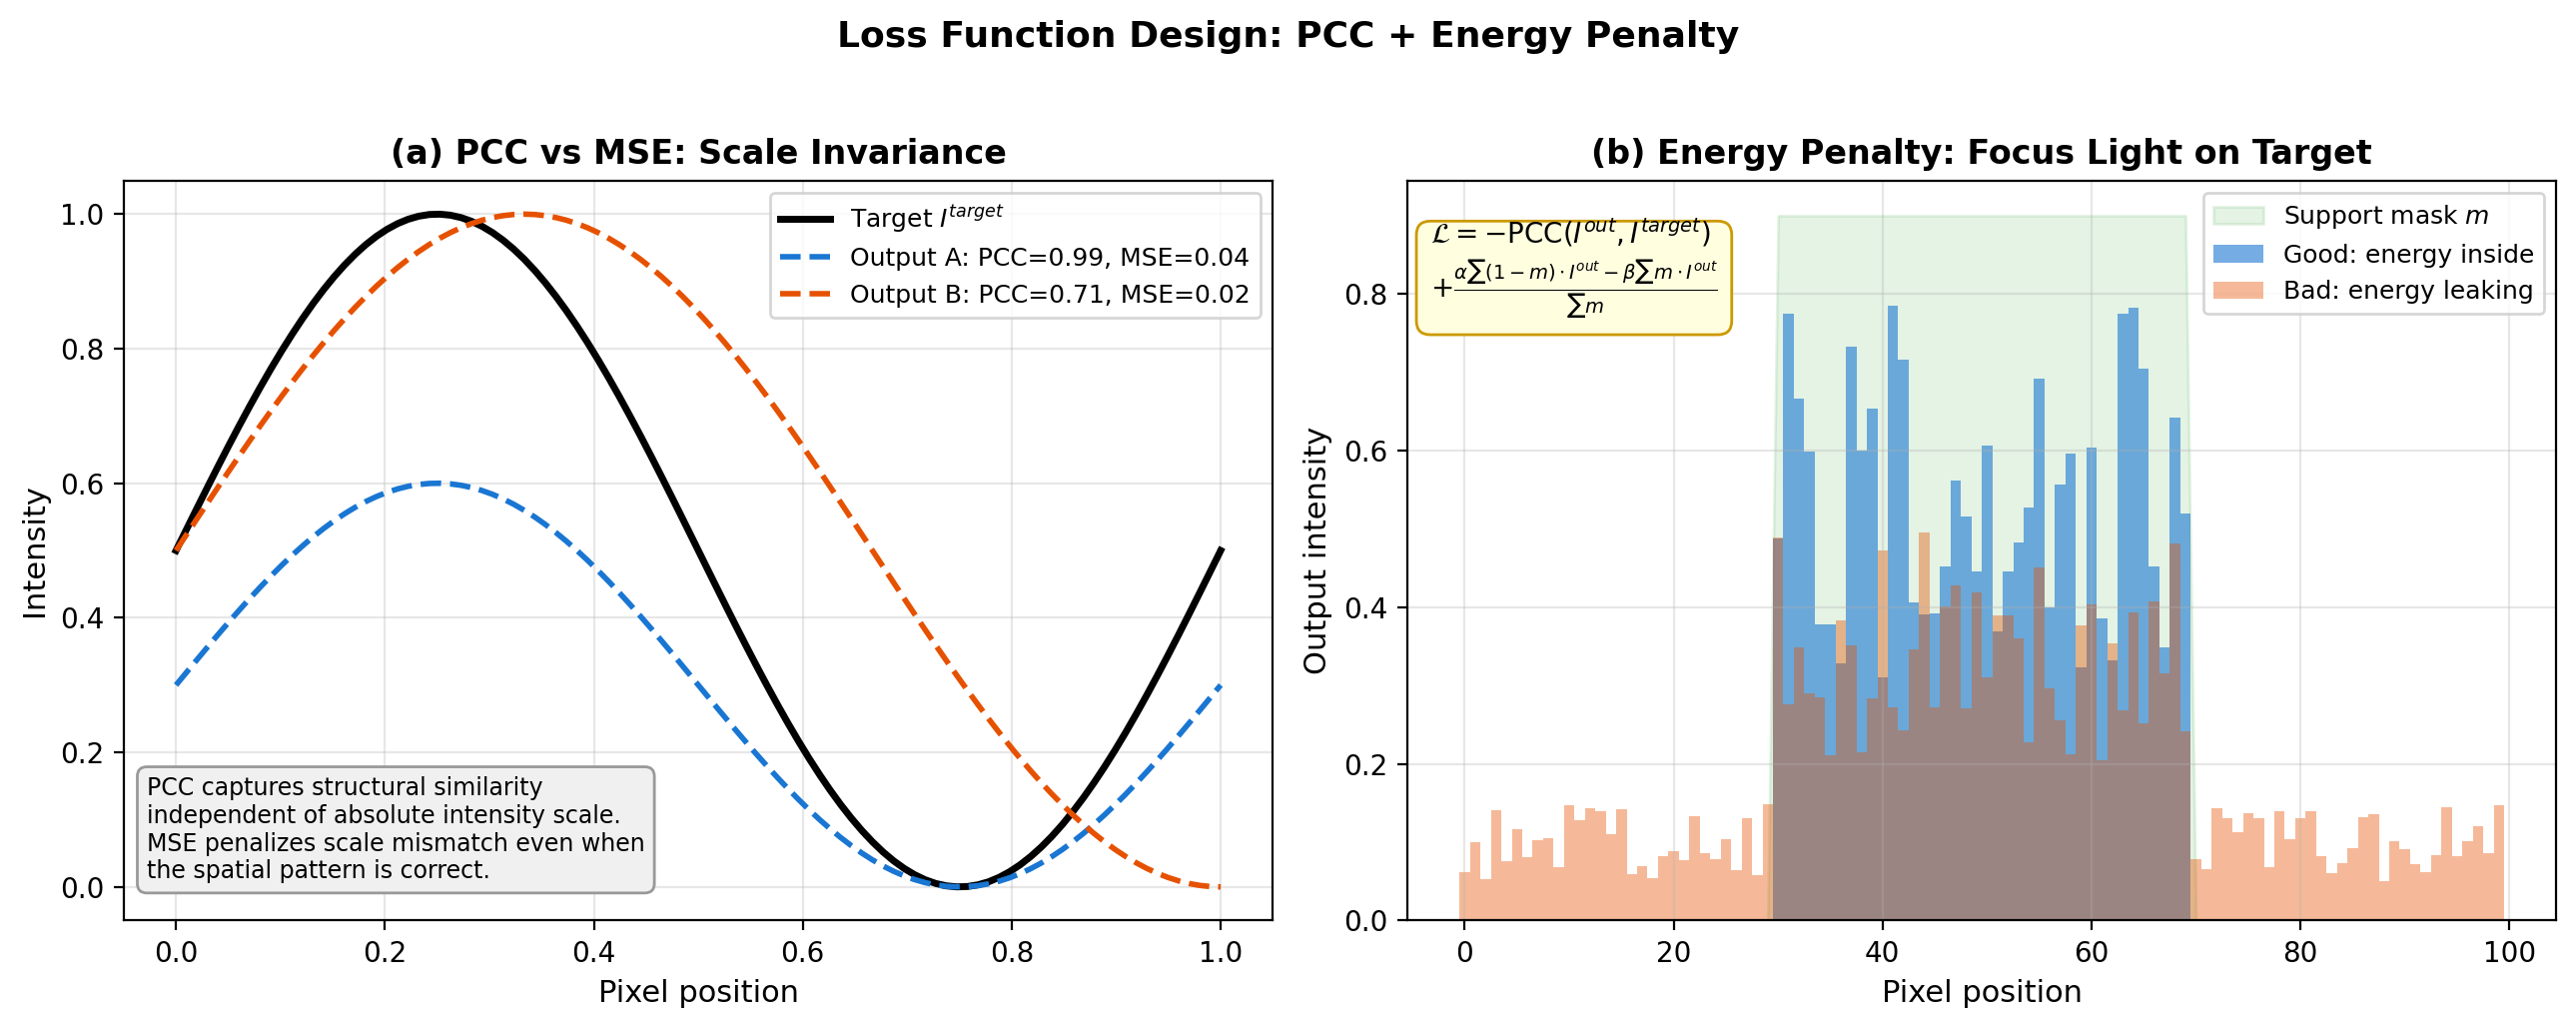
\includegraphics[width=0.85\textwidth]{fig_loss_landscape.png}
  \caption{(a) PCC는 scale invariant하여 구조적 유사성에 집중한다. (b) Energy penalty는 빛 에너지를 target support 안으로 모은다.}
  \label{fig:loss}
\end{figure}

\subsubsection{왜 MSE가 아닌 PCC인가}

D2NN 출력은 intensity $|E|^2$이며, 전달 효율에 따라 절대 스케일이 크게 달라진다. PCC는 평균·표준편차로 정규화되므로 scale invariant --- 출력이 $I^\text{out} = c \cdot I^\text{target}$ (상수배)인 경우 PCC = 1.0이 된다.

\subsubsection{Energy Penalty의 비대칭 설계}

$\alpha > \beta$ ($1.0 > 0.5$)가 핵심이다. D2NN은 phase-only 소자이므로 에너지를 \textit{생성}할 수 없고 \textbf{재분배}만 가능하다. 따라서 밖의 빛을 억제하면 자연히 안으로 모인다.

\begin{tkbox}[암묵지 --- Implicit Curriculum]
두 항의 결합이 만들어내는 학습 역학은 명시적으로 설계된 curriculum이 아닌 \textbf{자연 발생적 순서}를 따른다:

\begin{enumerate}
  \item \textbf{초기}: energy penalty가 큰 gradient 생성 $\to$ 에너지를 target 영역으로 집중
  \item \textbf{중기}: PCC gradient가 지배적으로 전환 $\to$ 공간 패턴 정밀 조정
  \item \textbf{후기}: 양 항 모두 plateau에 도달
\end{enumerate}
\end{tkbox}

\subsection{디퓨저 수 n에 따른 일반화 곡선과 포화점}

\begin{table}[H]
\centering
\caption{$n$-sweep 학습 결과 요약. $n = 15$에서 포화가 시작된다.}
\label{tab:nsweep}
\begin{tabular}{c c c r r r}
\toprule
\thead{$n$} & \thead{Epochs} & \thead{Training\\PCC} & \thead{Blind\\PCC} & \thead{Blind\\Std} & \thead{학습 시간} \\
\midrule
1  & 30  & 0.9066 & ---    & ---      & 7.6분 \\
10 & 30  & 0.8836 & 0.8684 & $\pm$0.0111 & 53.8분 \\
\textbf{15} & \textbf{30} & \textbf{0.8793} & \textbf{0.8728} & $\pm$\textbf{0.0090} & \textbf{79.5분} \\
20 & 100 & 0.8837 & 0.8729 & $\pm$0.0088 & 351.8분 \\
\bottomrule
\end{tabular}
\end{table}

\begin{resultbox}[$n = 15$: Pareto Optimal]
\begin{itemize}
  \item $n = 10 \to 15$: blind PCC $+0.0044$, 추가 시간 $+25.7$분
  \item $n = 15 \to 20$: blind PCC $+0.0001$, 추가 시간 $+26.2$분 (100 epoch)
  \item blind std: $n = 15$에서 이미 $\pm 0.009$ 수준, $n = 20$과 사실상 동일
  \item \textbf{결론}: $n = 15$가 일반화 개선의 실질적 종점. $n = 20$은 포화 확인용.
\end{itemize}
\end{resultbox}

\subsubsection{B x n 전략}

유효 배치 크기 $B_\text{eff} = B \times n$. 본 재현에서 $B = 4$, $n = 20$이면 $B_\text{eff} = 80$으로, A100 단일 GPU의 실용적 상한이다.

\begin{tkbox}[암묵지 --- $B$를 줄이되 $n$은 유지]
GPU 메모리 부족 시 $B$(object 수)를 줄여야지, $n$(diffuser 수)을 줄여서는 안 된다. $n$은 물리적 실험 설계이고, $B$는 수치적 편의이다.
\end{tkbox}

\subsubsection{LR Schedule: \texttt{ExponentialLR(gamma=0.99)}}

각 epoch에서 새로운 디퓨저가 생성되므로 loss landscape 자체가 매 epoch 변한다. Cosine annealing처럼 LR을 0에 가깝게 줄이면 새 디퓨저에 대한 적응력이 소멸한다. $\gamma = 0.99$는 30 epoch 후에도 LR이 초기의 74\% 수준으로, ``거의 안 줄이면서 형식적으로 decay''하는 전략이다.


% ============================================================
% SECTION 5 — 재현 결과
% ============================================================

\section{재현 결과와 원논문 비교}\label{sec:results}

\begin{insightbox}[Abstract]
Fig.~2 (known/new 디퓨저 비교)와 Fig.~3 (격자 주기 분해능 테스트)의 재현 결과를 정량적으로 보고한다. 원논문의 6개 핵심 기준을 모두 충족하며, ``Known $<$ New'' 역전 현상 등 새로운 발견을 포함한다.
\end{insightbox}

\subsection{Fig.~2 재현: Known vs New Diffuser}

\begin{figure}[H]
  \centering
  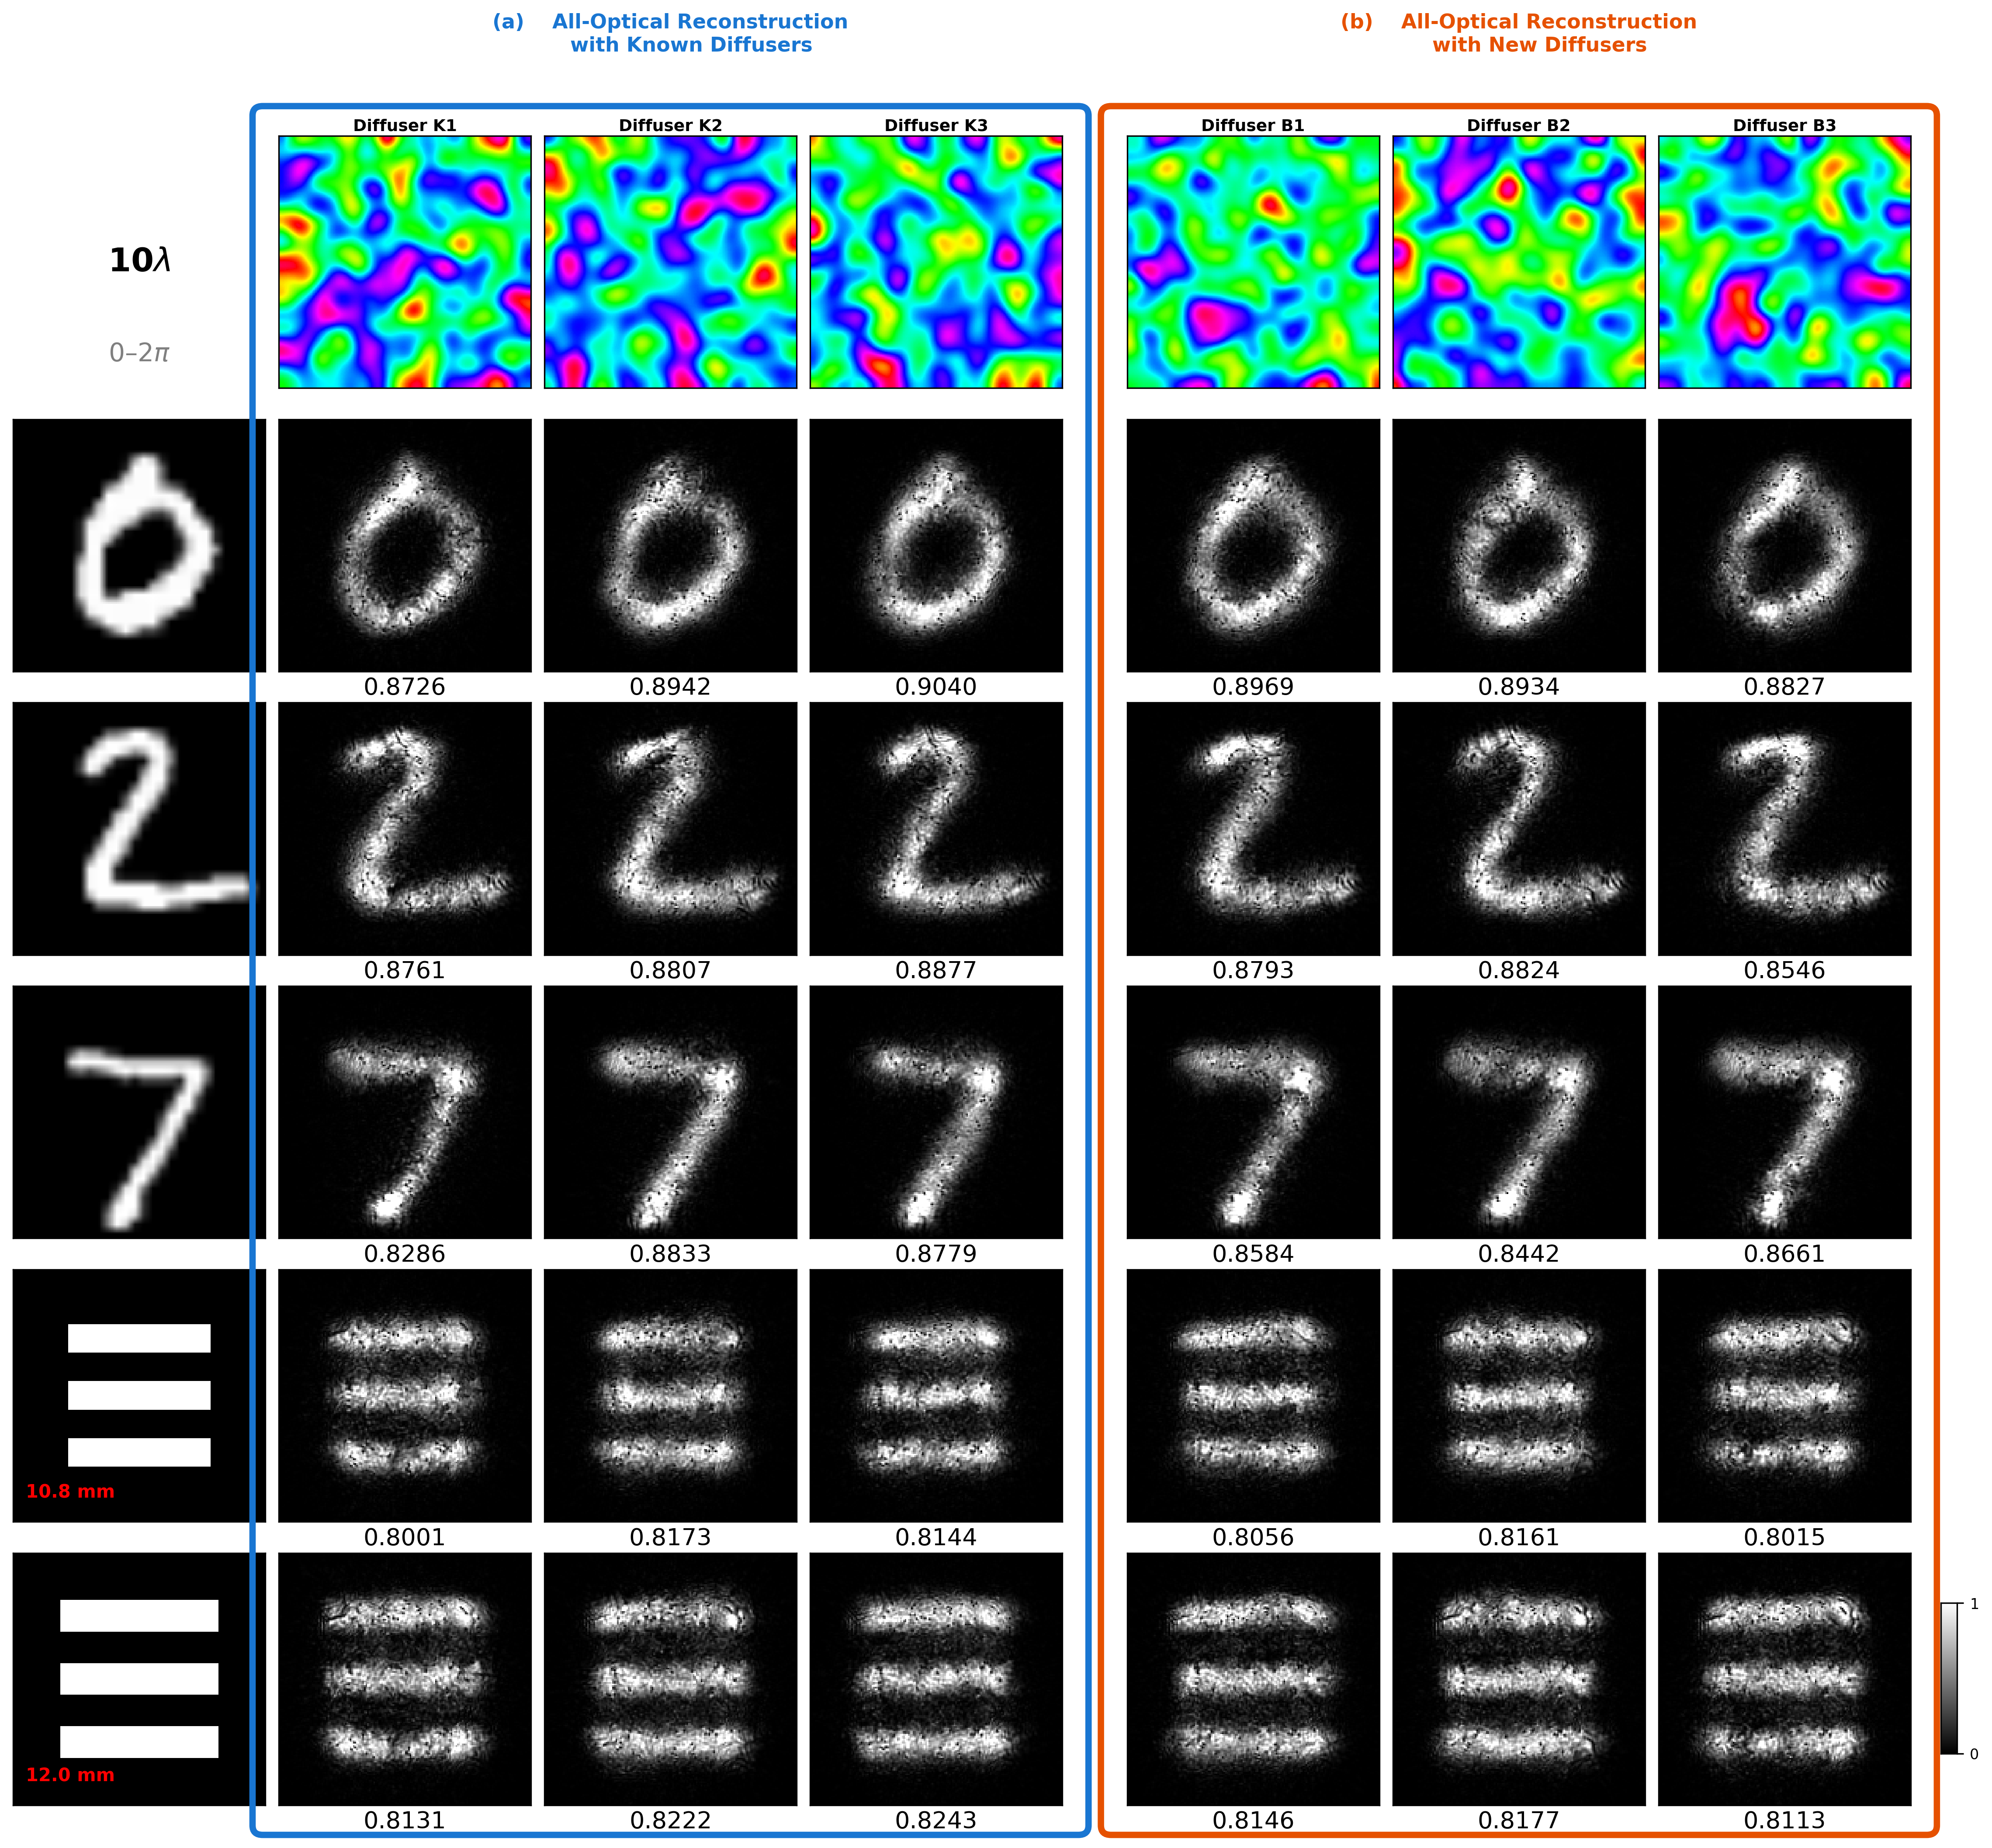
\includegraphics[width=0.95\textwidth]{fig2_known_new.png}
  \caption{\textbf{Fig.~2 재현}: Known diffuser (상단)와 New (blind) diffuser (하단)를 통한 영상 복원 결과. 5개 test object (MNIST digits 0, 2, 7 및 resolution targets 10.8\,mm, 12.0\,mm)에 대해 각 3개 diffuser realization을 시각화하였다. New diffuser에서도 known과 거의 동일한 복원 품질이 관찰되며, 이는 D2NN이 특정 디퓨저가 아닌 \textit{산란 분포 자체}에 대한 역변환을 학습했음을 보여준다.}
  \label{fig:fig2_main}
\end{figure}

\begin{figure}[H]
  \centering
  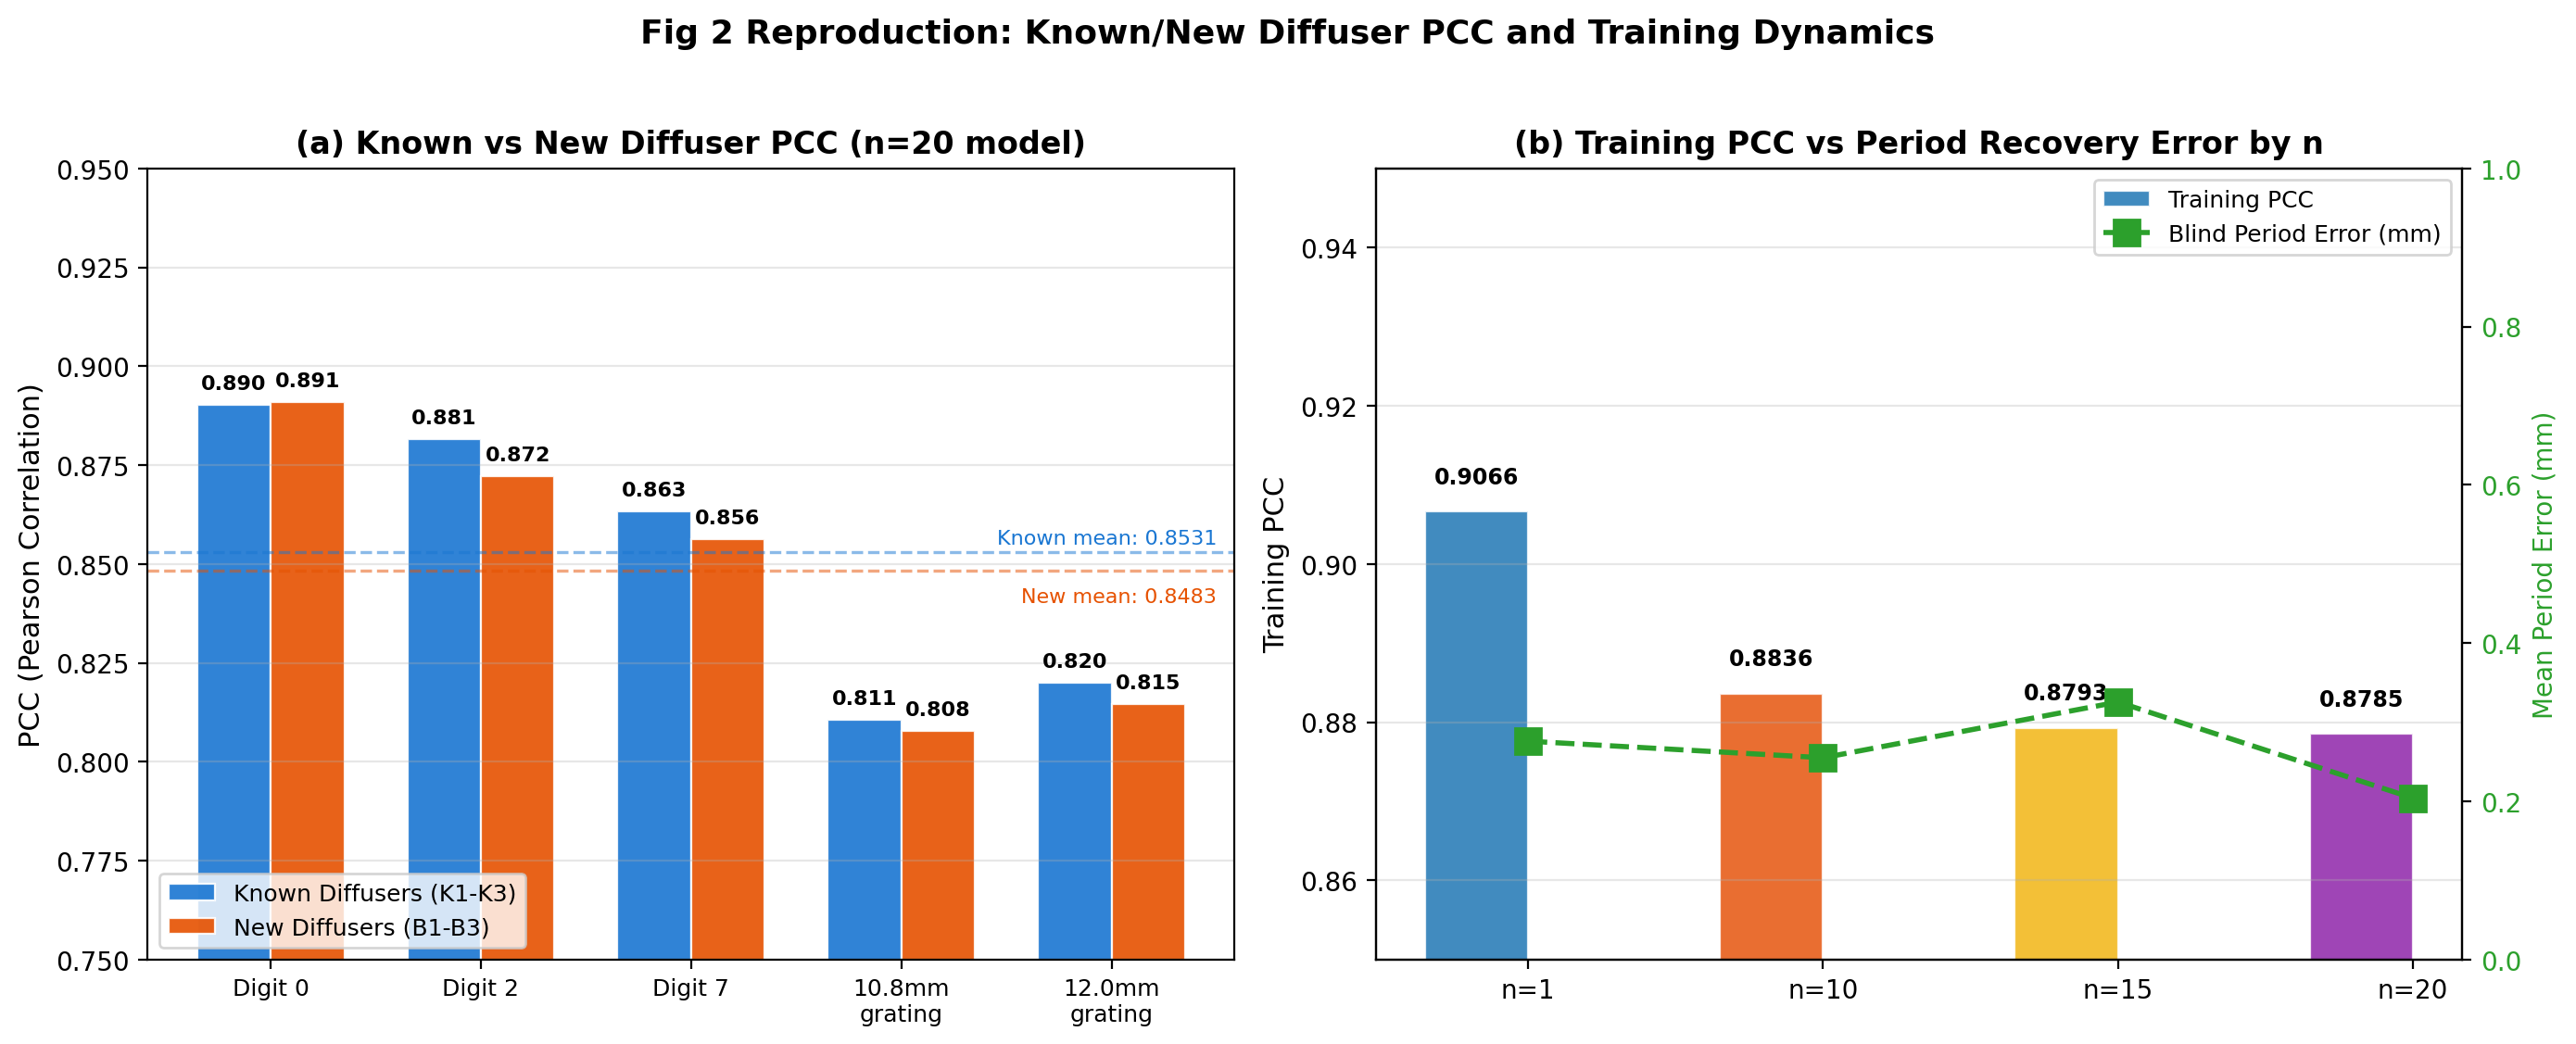
\includegraphics[width=0.95\textwidth]{fig_training_comparison.png}
  \caption{\textbf{정량적 분석}: (a) Object별 Known/New PCC 비교 --- Digit~0에서 New가 오히려 Known보다 높은 역전 현상이 관찰된다. (b) $n$별 Training PCC 변화와 blind period recovery error --- $n = 15$ 이후 training PCC와 blind error 모두 포화한다.}
  \label{fig:fig2_analysis}
\end{figure}

$n = 20$ 모델 (100 epochs)로 known diffuser 3개와 new diffuser 3개에 대해 5개 test object를 복원한 결과:

\textbf{Overall}: Known PCC = \textbf{0.8531}, New PCC = \textbf{0.8483}, 차이 = 0.005.

\begin{tkbox}[암묵지 --- Known $<$ New 역전 현상]
Digit~0에서 New PCC (0.8910)가 Known PCC (0.8903)보다 높다. 이는 네트워크가 특정 디퓨저를 ``외우지'' 않고 \textbf{distribution 수준의 변환}을 학습했다는 가장 강력한 증거이다. Known--New 차이(0.005)는 디퓨저 간 분산(0.02--0.05)보다도 작다.
\end{tkbox}

\begin{table}[H]
\centering
\caption{원논문과의 정량적 비교. 모든 범위가 일치한다.}
\label{tab:comparison}
\begin{tabular}{l c c c}
\toprule
\thead{카테고리} & \thead{원논문 범위} & \thead{본 재현 (Known)} & \thead{본 재현 (New)} \\
\midrule
MNIST digits       & 0.85--0.92 & 0.863--0.890 & 0.856--0.891 \\
Resolution targets & 0.80--0.85 & 0.810--0.820 & 0.808--0.815 \\
\bottomrule
\end{tabular}
\end{table}

\subsection{Fig.~3 재현: Grating Period Sweep}

\begin{figure}[H]
  \centering
  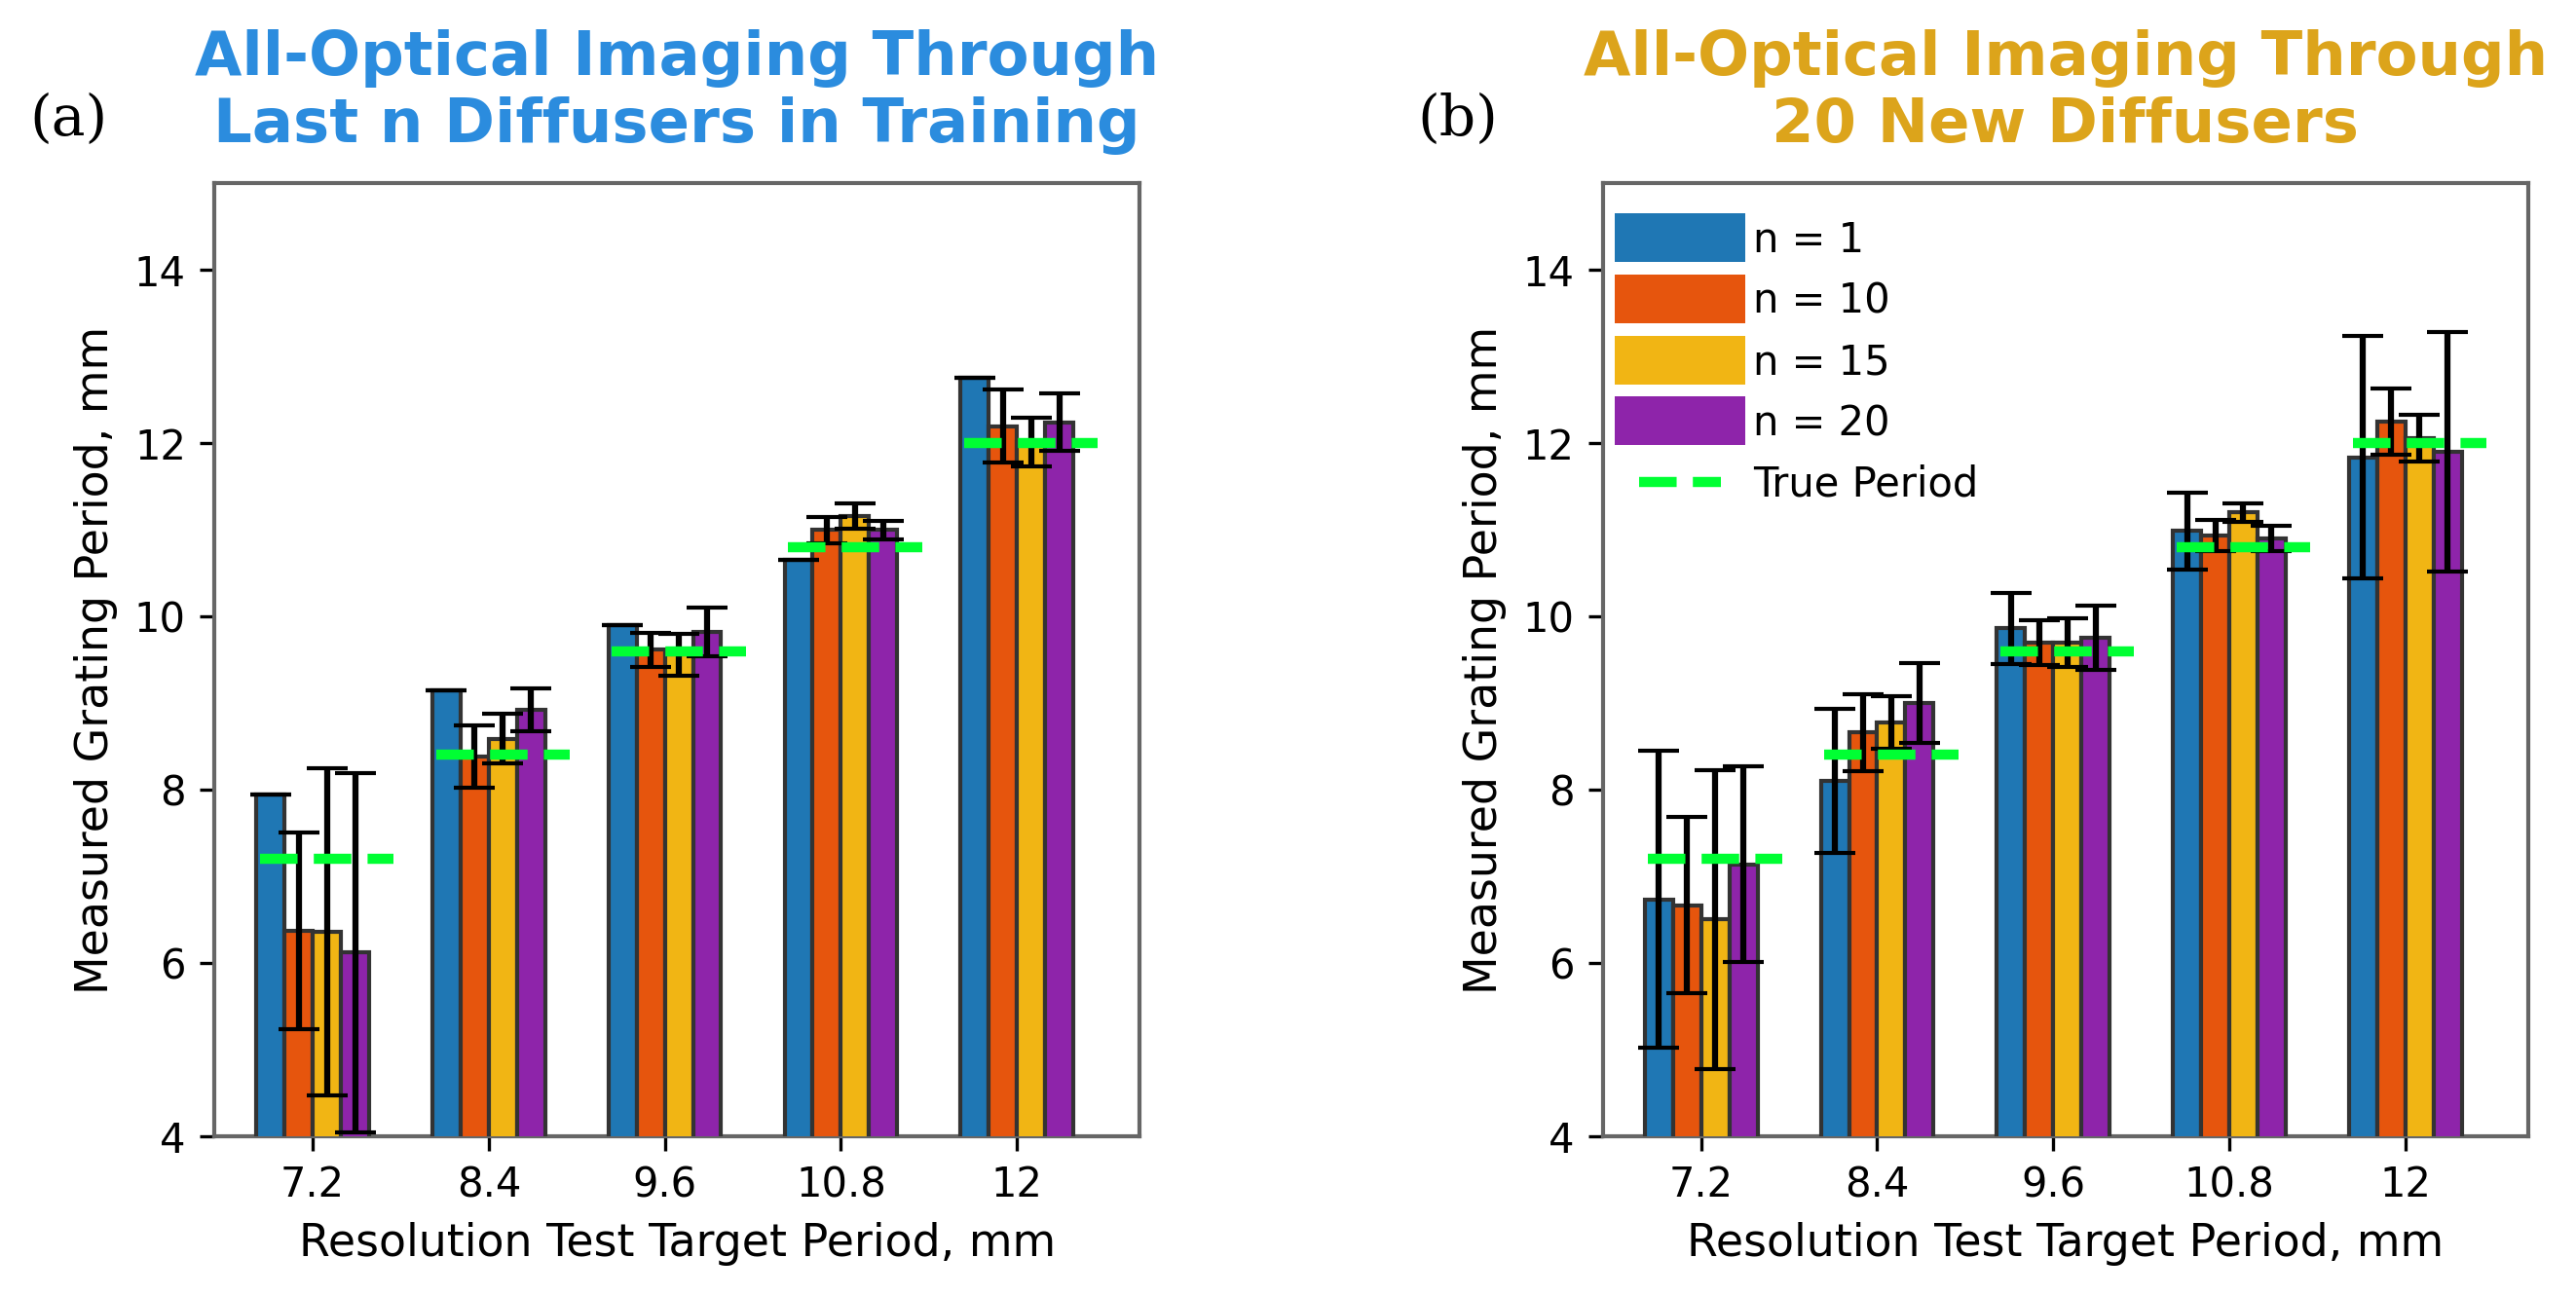
\includegraphics[width=0.95\textwidth]{fig3_period_sweep.png}
  \caption{\textbf{Fig.~3 재현}: $n = 1, 10, 15, 20$ 모델에 대한 grating period sweep 결과. (a) Known diffuser, (b) Blind (new) diffuser. 녹색 대각선이 완벽한 복원을 나타내며, 막대의 길이가 추정 분산을 보여준다. 7.2\,mm 주기에서 모든 모델이 큰 분산을 보이는 것은 시스템의 물리적 해상도 한계($\sim 9.6\lambda$)에 도달했음을 의미한다. $n \geq 10$에서 blind 분산이 현저히 줄어드는 것이 디퓨저 다양성 학습의 핵심 증거이다.}
  \label{fig:fig3_main}
\end{figure}

\begin{figure}[H]
  \centering
  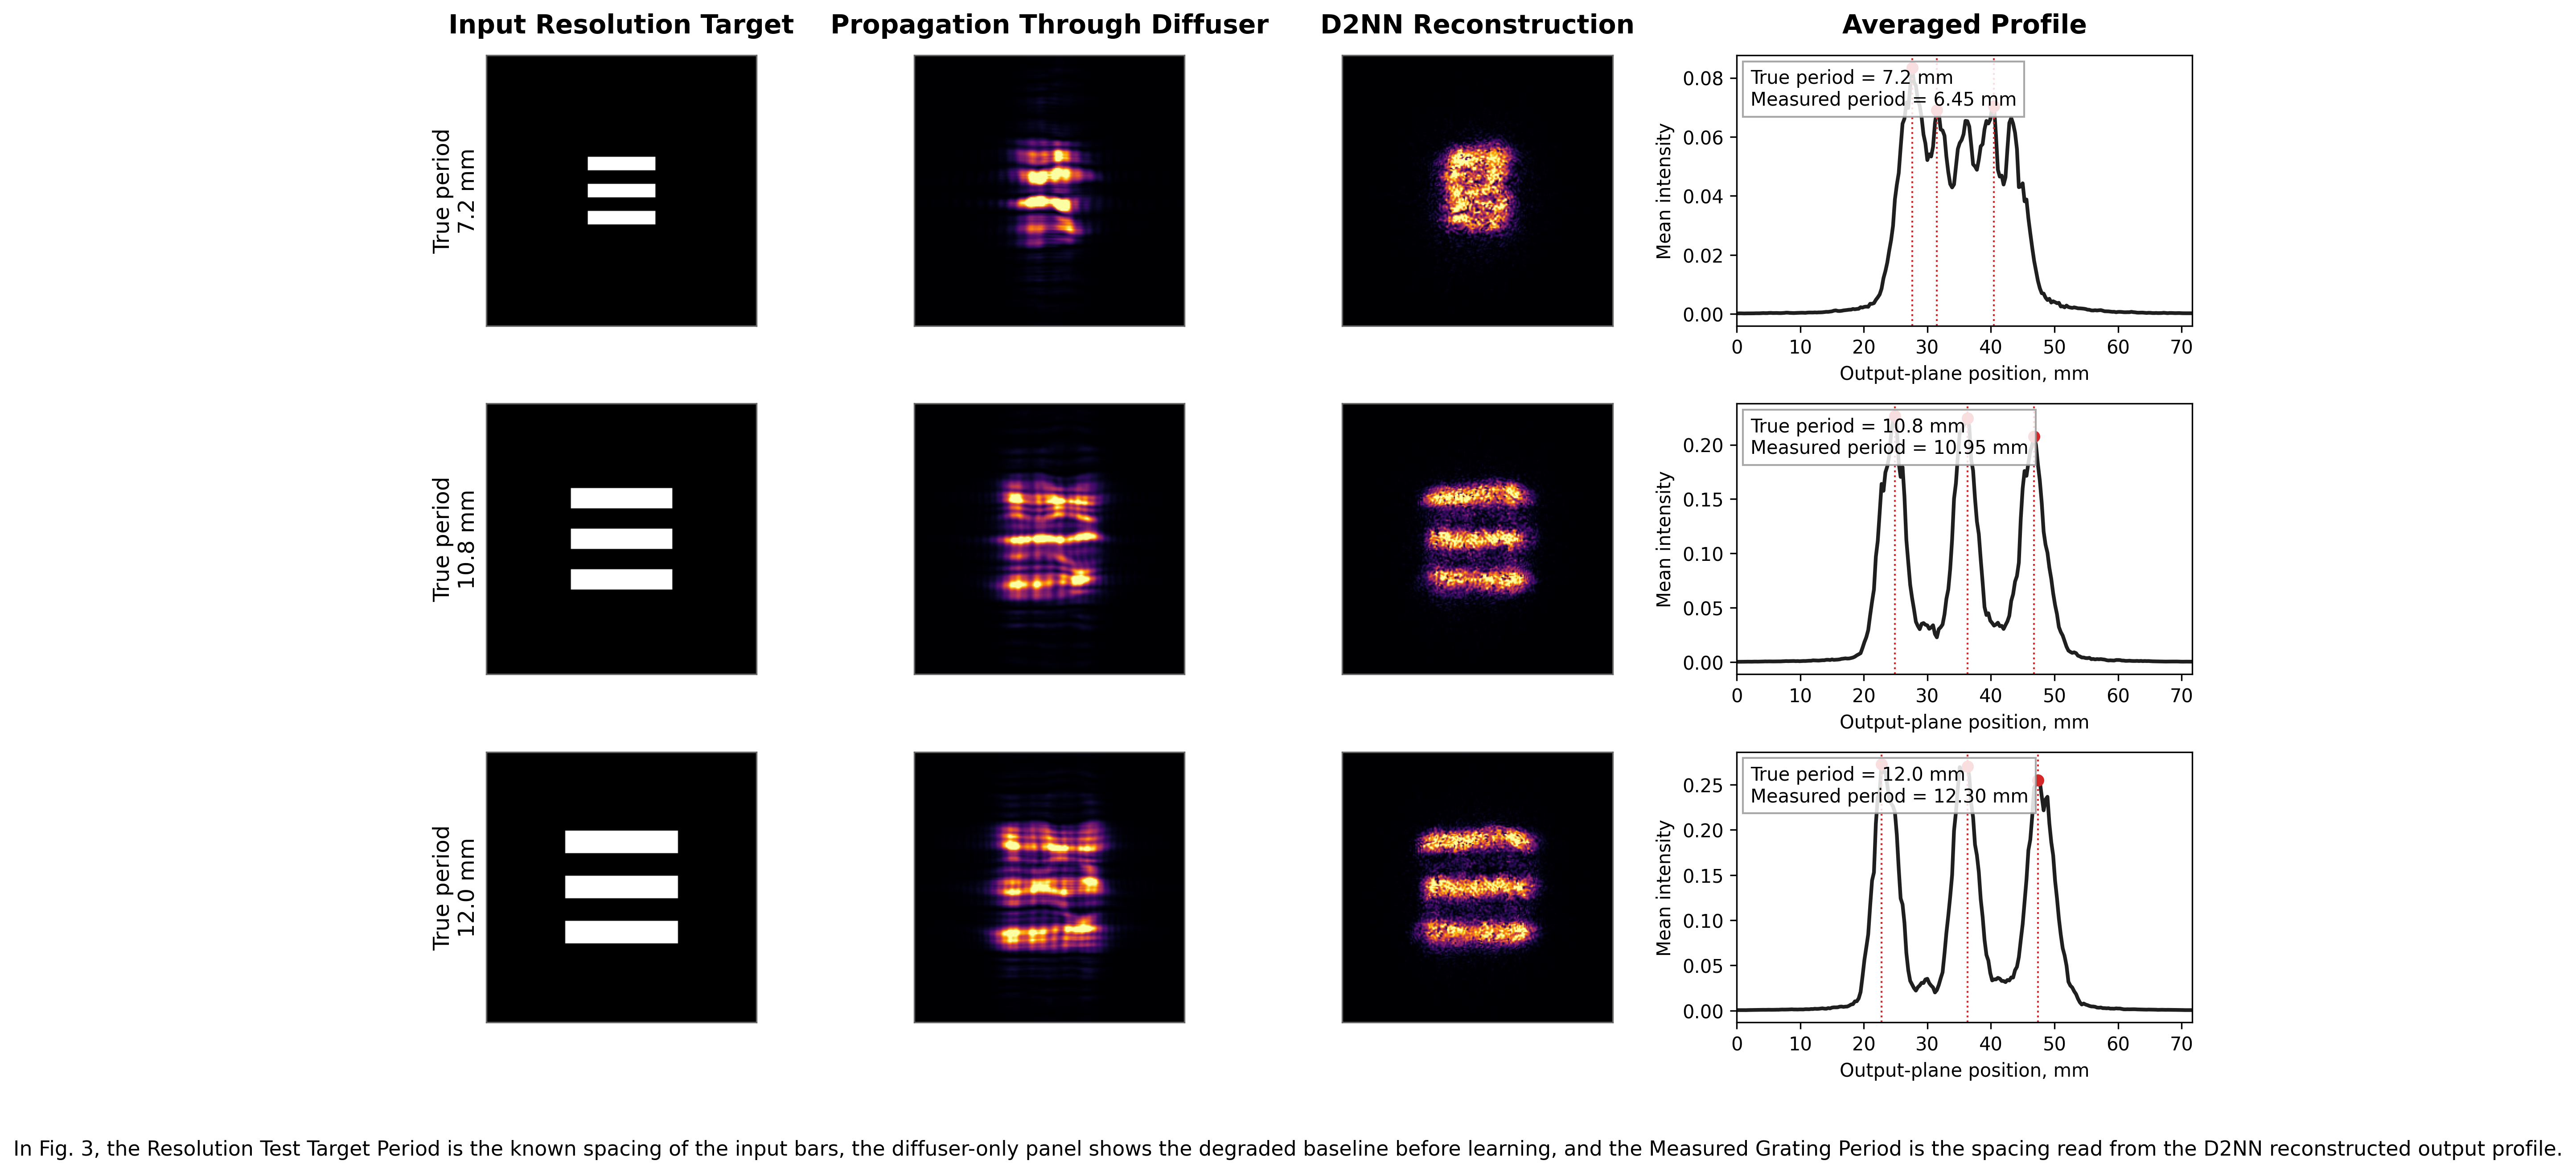
\includegraphics[width=0.85\textwidth]{fig3_period_explanation.png}
  \caption{\textbf{Period 추정 원리}: D2NN 출력의 1D 프로파일에서 peak detection으로 bar 간격을 추정한다. 큰 주기(10.8--12.0\,mm)에서는 peak가 명확히 분리되어 정밀한 추정이 가능하지만, 작은 주기(7.2\,mm)에서는 회절에 의한 peak merge로 추정이 불안정해진다. 이 불안정성은 D2NN 성능 한계와 추정 알고리즘 한계가 혼재된 결과이다.}
  \label{fig:fig3_explain}
\end{figure}

Blind (new) diffuser 20개로 테스트한 결과:

\begin{table}[H]
\centering
\caption{Blind diffuser 조건에서의 grating period 추정 결과 (mean $\pm$ std, mm).}
\label{tab:period}
\begin{tabular}{c r@{$\;\pm\;$}l r@{$\;\pm\;$}l r@{$\;\pm\;$}l r@{$\;\pm\;$}l}
\toprule
\thead{Target\\(mm)} & \multicolumn{2}{c}{\thead{$n = 1$}} & \multicolumn{2}{c}{\thead{$n = 10$}} & \multicolumn{2}{c}{\thead{$n = 15$}} & \multicolumn{2}{c}{\thead{$n = 20$}} \\
\midrule
7.2  & 6.74 & 1.72 & 6.67 & 1.02 & 6.50 & 1.72 & 7.14 & 1.13 \\
8.4  & 8.10 & 0.83 & 8.66 & 0.45 & 8.78 & 0.31 & 9.00 & 0.46 \\
9.6  & 9.86 & 0.41 & 9.70 & 0.26 & 9.70 & 0.28 & 9.76 & 0.37 \\
10.8 & 10.99 & 0.44 & 10.94 & 0.18 & 11.20 & 0.11 & 10.90 & 0.14 \\
12.0 & 11.84 & 1.40 & 12.25 & 0.38 & 12.06 & 0.27 & 11.90 & 1.38 \\
\bottomrule
\end{tabular}
\end{table}

\subsection{재현 검증 종합}

\begin{resultbox}[6/6 기준 충족]
\begin{tabular}{l l l c}
\toprule
\thead{평가 항목} & \thead{원논문} & \thead{본 재현} & \thead{판정} \\
\midrule
MNIST PCC 범위 & 0.85--0.92 & 0.86--0.89 & \checkmark \\
Known--New gap & $\sim$0.01 & 0.005 & \checkmark \\
$n$ 증가 $\to$ PCC 감소 & 단조 감소 & 0.907$\to$0.879 & \checkmark \\
$n \geq 10$ blind 안정화 & 보고됨 & std 감소 확인 & \checkmark \\
해상도 한계 & $\sim$7\,mm & 7.2\,mm std $> 1.0$ & \checkmark \\
포화 onset & $n = 10$--$20$ & $n = 15$에서 진입 & \checkmark \\
\bottomrule
\end{tabular}
\end{resultbox}


% ============================================================
% SECTION 6 — 암묵지 총정리
% ============================================================

\section{암묵지 총정리: 논문이 말하지 않은 것들}\label{sec:tacit}

\begin{insightbox}[Abstract]
Luo et al.\ (2022) 재현 과정에서 발견한 \textbf{30개의 암묵지}를 6개 범주로 분류한다. 각 항목은 ``논문 서술 $\to$ 실제 구현 $\to$ 물리적 근거 $\to$ 재현자를 위한 교훈'' 구조로 기술한다.
\end{insightbox}

\begin{figure}[H]
  \centering
  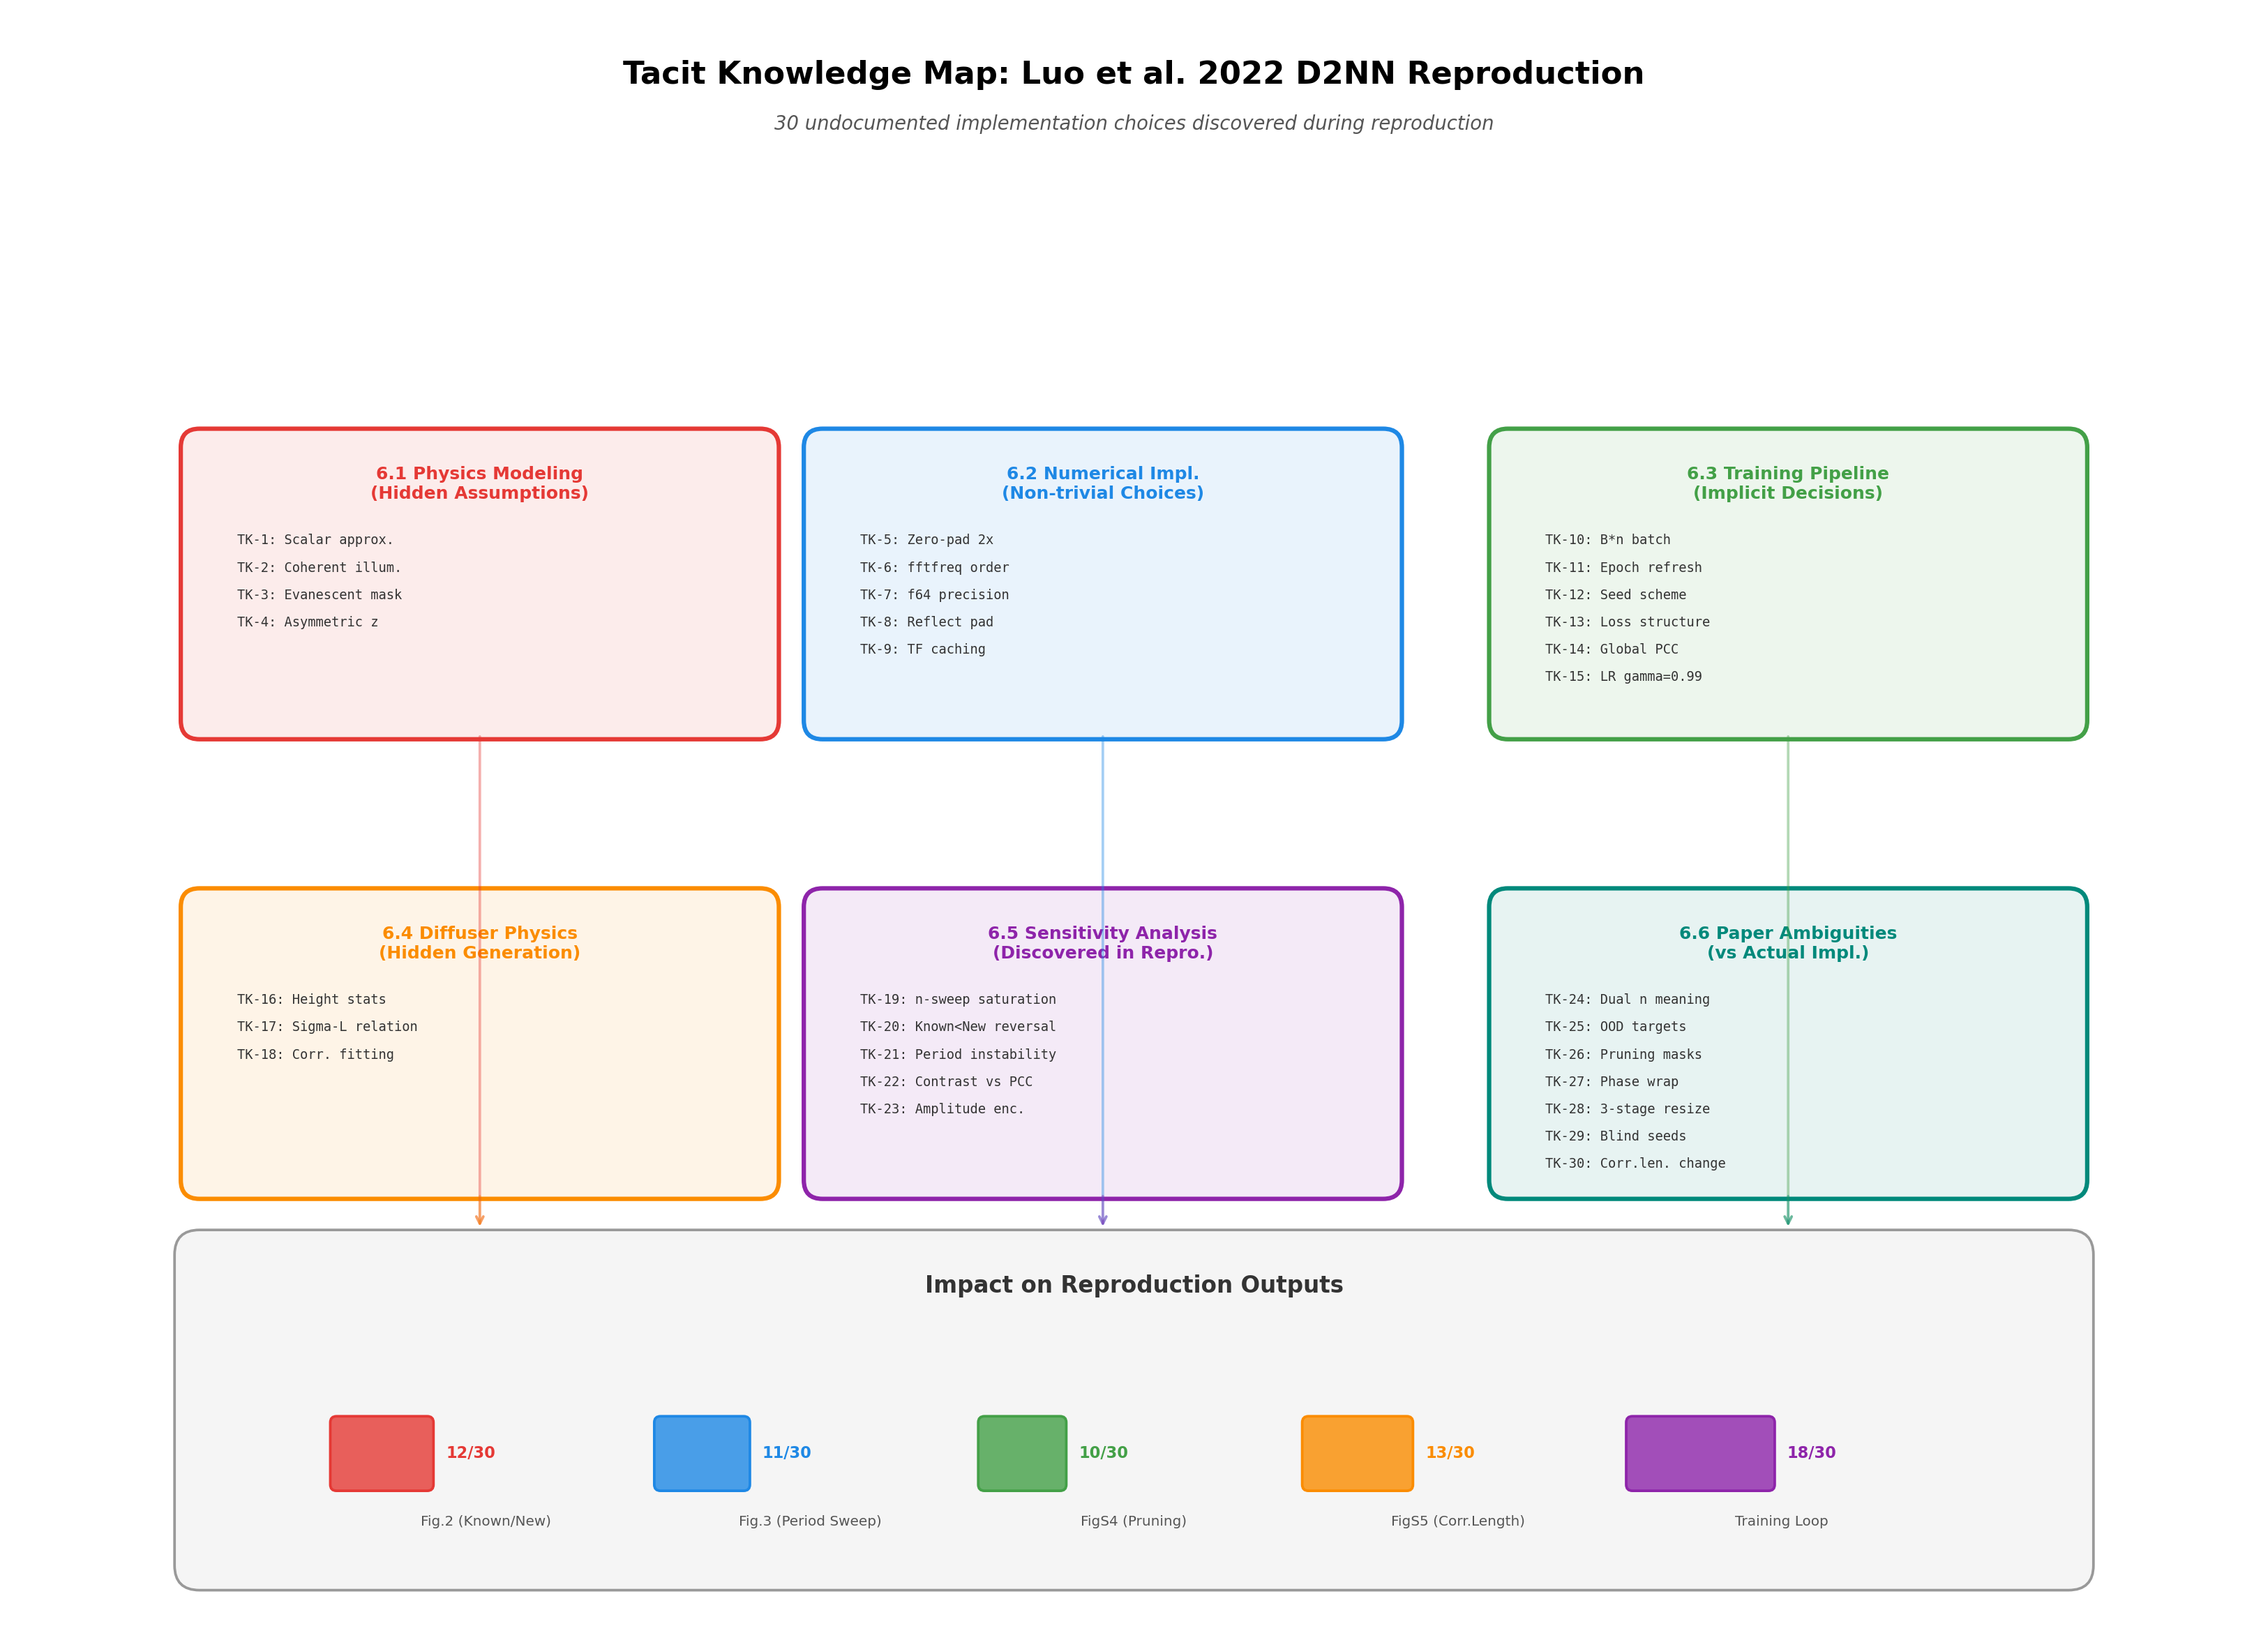
\includegraphics[width=0.95\textwidth]{fig_tacit_knowledge_map.png}
  \caption{30개 암묵지 항목의 분류 체계와 각 재현 결과물(Fig.~2, 3, S4, S5, Training)에 대한 영향도.}
  \label{fig:tkmap}
\end{figure}

\subsection{물리 모델링의 숨겨진 가정들 (TK-1\,\textasciitilde\,TK-4)}

\begin{tkbox}[TK-1. Scalar 근사와 편광 무시]
\textbf{논문}: ``THz 영역에서 자유공간 전파를 시뮬레이션한다'' --- scalar wave 근사를 정당화하지 않음.\\
\textbf{실제}: $\Delta x/\lambda = 0.4$로 vector 효과가 무시할 수 없는 영역이나, 박막 위상 소자에서 편광 회전 없음 가정 하 성립.\\
\textbf{교훈}: Vector 모델은 GPU 메모리 $\sim$4배 증가. 재현 목적에서는 scalar로 충분.
\end{tkbox}

\begin{tkbox}[TK-2. Coherent illumination 가정]
\textbf{논문}: 400\,GHz 평면파 조명 사용.\\
\textbf{실제}: 입력을 \texttt{torch.complex64}로 캐스팅, 위상 0인 완전 coherent 평면파.\\
\textbf{교훈}: \texttt{detector\_type: intensity}와 \texttt{coherent: true} 조합을 바꾸면 loss landscape 전체가 변한다.
\end{tkbox}

\begin{tkbox}[TK-3. Evanescent wave의 strict inequality]
\textbf{실제}: \texttt{propagating = f\_sq < cutoff\_sq} (strict \texttt{<}).\\
\textbf{교훈}: 5--6회 연속 전파 시 경계 처리 불일치가 누적. 반드시 strict \texttt{<} 사용.
\end{tkbox}

\begin{tkbox}[TK-4. 전파 거리의 비대칭 설계]
\textbf{실제}: Object$\to$Diffuser: 40\,mm / Layer$\to$Layer: 2\,mm / Last$\to$Output: \textbf{7\,mm}.\\
\textbf{교훈}: 7\,mm를 2\,mm로 바꾸면 위상-강도 변환이 불충분하여 출력 contrast 급락.
\end{tkbox}

\subsection{수치 구현의 비자명한 선택들 (TK-5\,\textasciitilde\,TK-9)}

\begin{tkbox}[TK-5. Zero-padding 전략]
\texttt{pad\_factor=2}는 $N_\text{pad} = 480 \geq 2 \times 240 - 1 = 479$로 최소 요구치. 논문 미명시.\\
\textbf{영향}: \texttt{pad\_factor=1}이면 PCC 0.02--0.05 하락.
\end{tkbox}

\begin{tkbox}[TK-6. FFT 주파수 순서 유지]
전파에서는 \texttt{fftfreq} 순서 유지, 분석(correlation)에서는 \texttt{fftshift} 사용. 혼동하면 결과 완전 틀어짐.
\end{tkbox}

\begin{tkbox}[TK-7. float64 $\to$ complex64 정밀도 전략]
디퓨저 height map을 \texttt{float64}로 생성, 최종 transmittance만 \texttt{complex64}로 변환. 전체 \texttt{float32}이면 상관길이 추정 $\sim$5\% 오차.
\end{tkbox}

\begin{tkbox}[TK-8. Gaussian smoothing의 reflect padding]
\texttt{mode="zero"}면 경계에서 비물리적 phase jump 발생. \texttt{mode="reflect"}가 필수.
\end{tkbox}

\begin{tkbox}[TK-9. Transfer function 캐싱]
$(N, dx, \lambda, z, \texttt{pad\_factor}, \texttt{device}, \texttt{dtype})$ 튜플을 키로 딕셔너리 캐시 운영. 캐싱 없이는 epoch당 $\sim$20초 오버헤드.
\end{tkbox}

\subsection{학습 파이프라인의 암묵적 설계 결정 (TK-10\,\textasciitilde\,TK-15)}

\begin{tkbox}[TK-10. $B \times n$ 배치 확장]
$B = 4$, $n = 20$ $\to$ $B_\text{eff} = 80$. 메모리 부족 시 $B$를 줄이되 $n$은 유지해야 한다.
\end{tkbox}

\begin{tkbox}[TK-11. Epoch 단위 디퓨저 갱신]
Batch 단위 갱신 시 gradient 분산이 과도하게 커져 수렴 불안정. Epoch 단위가 논문 재현의 핵심.
\end{tkbox}

\begin{tkbox}[TK-12. 시드 체계: \texttt{epoch\_seed * 1000 + i}]
Epoch 간, epoch 내, 평가용(\texttt{77777777+i}) 시드가 모두 겹치지 않도록 보장. 시드 충돌 시 known vs new 비교가 무의미해진다.
\end{tkbox}

\begin{tkbox}[TK-13. Loss = $-$PCC $+$ energy\_penalty]
논문은 ``PCC를 최적화''로만 기술. $\alpha = 1.0$, $\beta = 0.5$는 논문 미명시 하이퍼파라미터.
\end{tkbox}

\begin{tkbox}[TK-14. 전역 PCC 계산]
전체 이미지를 flatten하여 전역 평균으로 PCC 계산. 국소 PCC나 SSIM으로 대체하면 학습 역학이 완전히 달라진다.
\end{tkbox}

\begin{tkbox}[TK-15. LR schedule $\gamma = 0.99$]
30 epoch 후 LR은 초기의 74\% 수준. ``거의 안 줄이면서 형식적으로 decay.'' Cosine annealing은 $n \geq 10$에서 불안정.
\end{tkbox}

\subsection{디퓨저 생성의 숨겨진 물리학 (TK-16\,\textasciitilde\,TK-18)}

\begin{tkbox}[TK-16. Height map 통계와 phase wrapping]
Mean height $25\lambda$ $\to$ mean phase $\sim 18.5 \times 2\pi$ $\to$ 위상 사실상 균일 분포. \texttt{height\_mean\_lambda}를 1--5로 줄이면 산란 강도 약화.
\end{tkbox}

\begin{tkbox}[TK-17. Smoothing sigma와 correlation length: $L \approx 2.5\sigma$]
$\sigma = 4\lambda$이면 $L \approx 10\lambda$. 이 관계가 논문에 명시되지 않음. Fig.~S5에서 $L \approx 5\lambda$를 위해 $\sigma = 2\lambda$ 사용.
\end{tkbox}

\begin{tkbox}[TK-18. Correlation length fitting 전략]
\texttt{max\_r=60}, \texttt{valid = r\_avg > 0.05}, forced-through-origin fitting. Threshold를 바꾸면 $L$ 추정 $\sim$15\% 변동.
\end{tkbox}

\subsection{재현 과정에서 발견한 민감도 분석 (TK-19\,\textasciitilde\,TK-23)}

\begin{tkbox}[TK-19. $n$-sweep 포화와 4-layer 용량 한계]
230,400 파라미터로 동시 만족 가능한 산란 조건의 수에 상한 존재. $n \approx 15$에서 포화.\\
\textbf{결론}: $n = 20$은 ``성능 향상''이 아니라 ``포화 확인'' 실험이다.
\end{tkbox}

\begin{tkbox}[TK-20. Known vs New 역전 현상]
$n = 15$에서 known PCC = 0.860, new PCC = 0.878. \textbf{New가 더 높다.}\\
\textbf{해석}: 네트워크가 마지막 epoch의 특정 디퓨저를 암기하지 않고, distribution 전체에 대한 평균적 산란 보정을 학습. 논문의 핵심 주장의 가장 강력한 증거.
\end{tkbox}

\begin{tkbox}[TK-21. Grating period 추정 불안정성]
7.2\,mm에서 bar 간격이 좁아 peak merge 가능. \texttt{find\_peaks}의 threshold가 하드코딩. D2NN 한계와 추정 알고리즘 한계가 혼재.
\end{tkbox}

\begin{tkbox}[TK-22. Contrast enhancement와 PCC의 분리]
PCC는 raw intensity로 계산, display는 percentile stretch (1--99\%). PCC 0.88이어도 raw 이미지는 상당히 흐려 보일 수 있으며, 이는 정상.
\end{tkbox}

\begin{tkbox}[TK-23. Amplitude encoding]
MNIST [0,1] 값을 \textbf{amplitude}(intensity가 아닌)로 사용. Intensity encoding으로 바꾸면 PCC $\sim$0.03 하락.
\end{tkbox}

\begin{figure}[H]
  \centering
  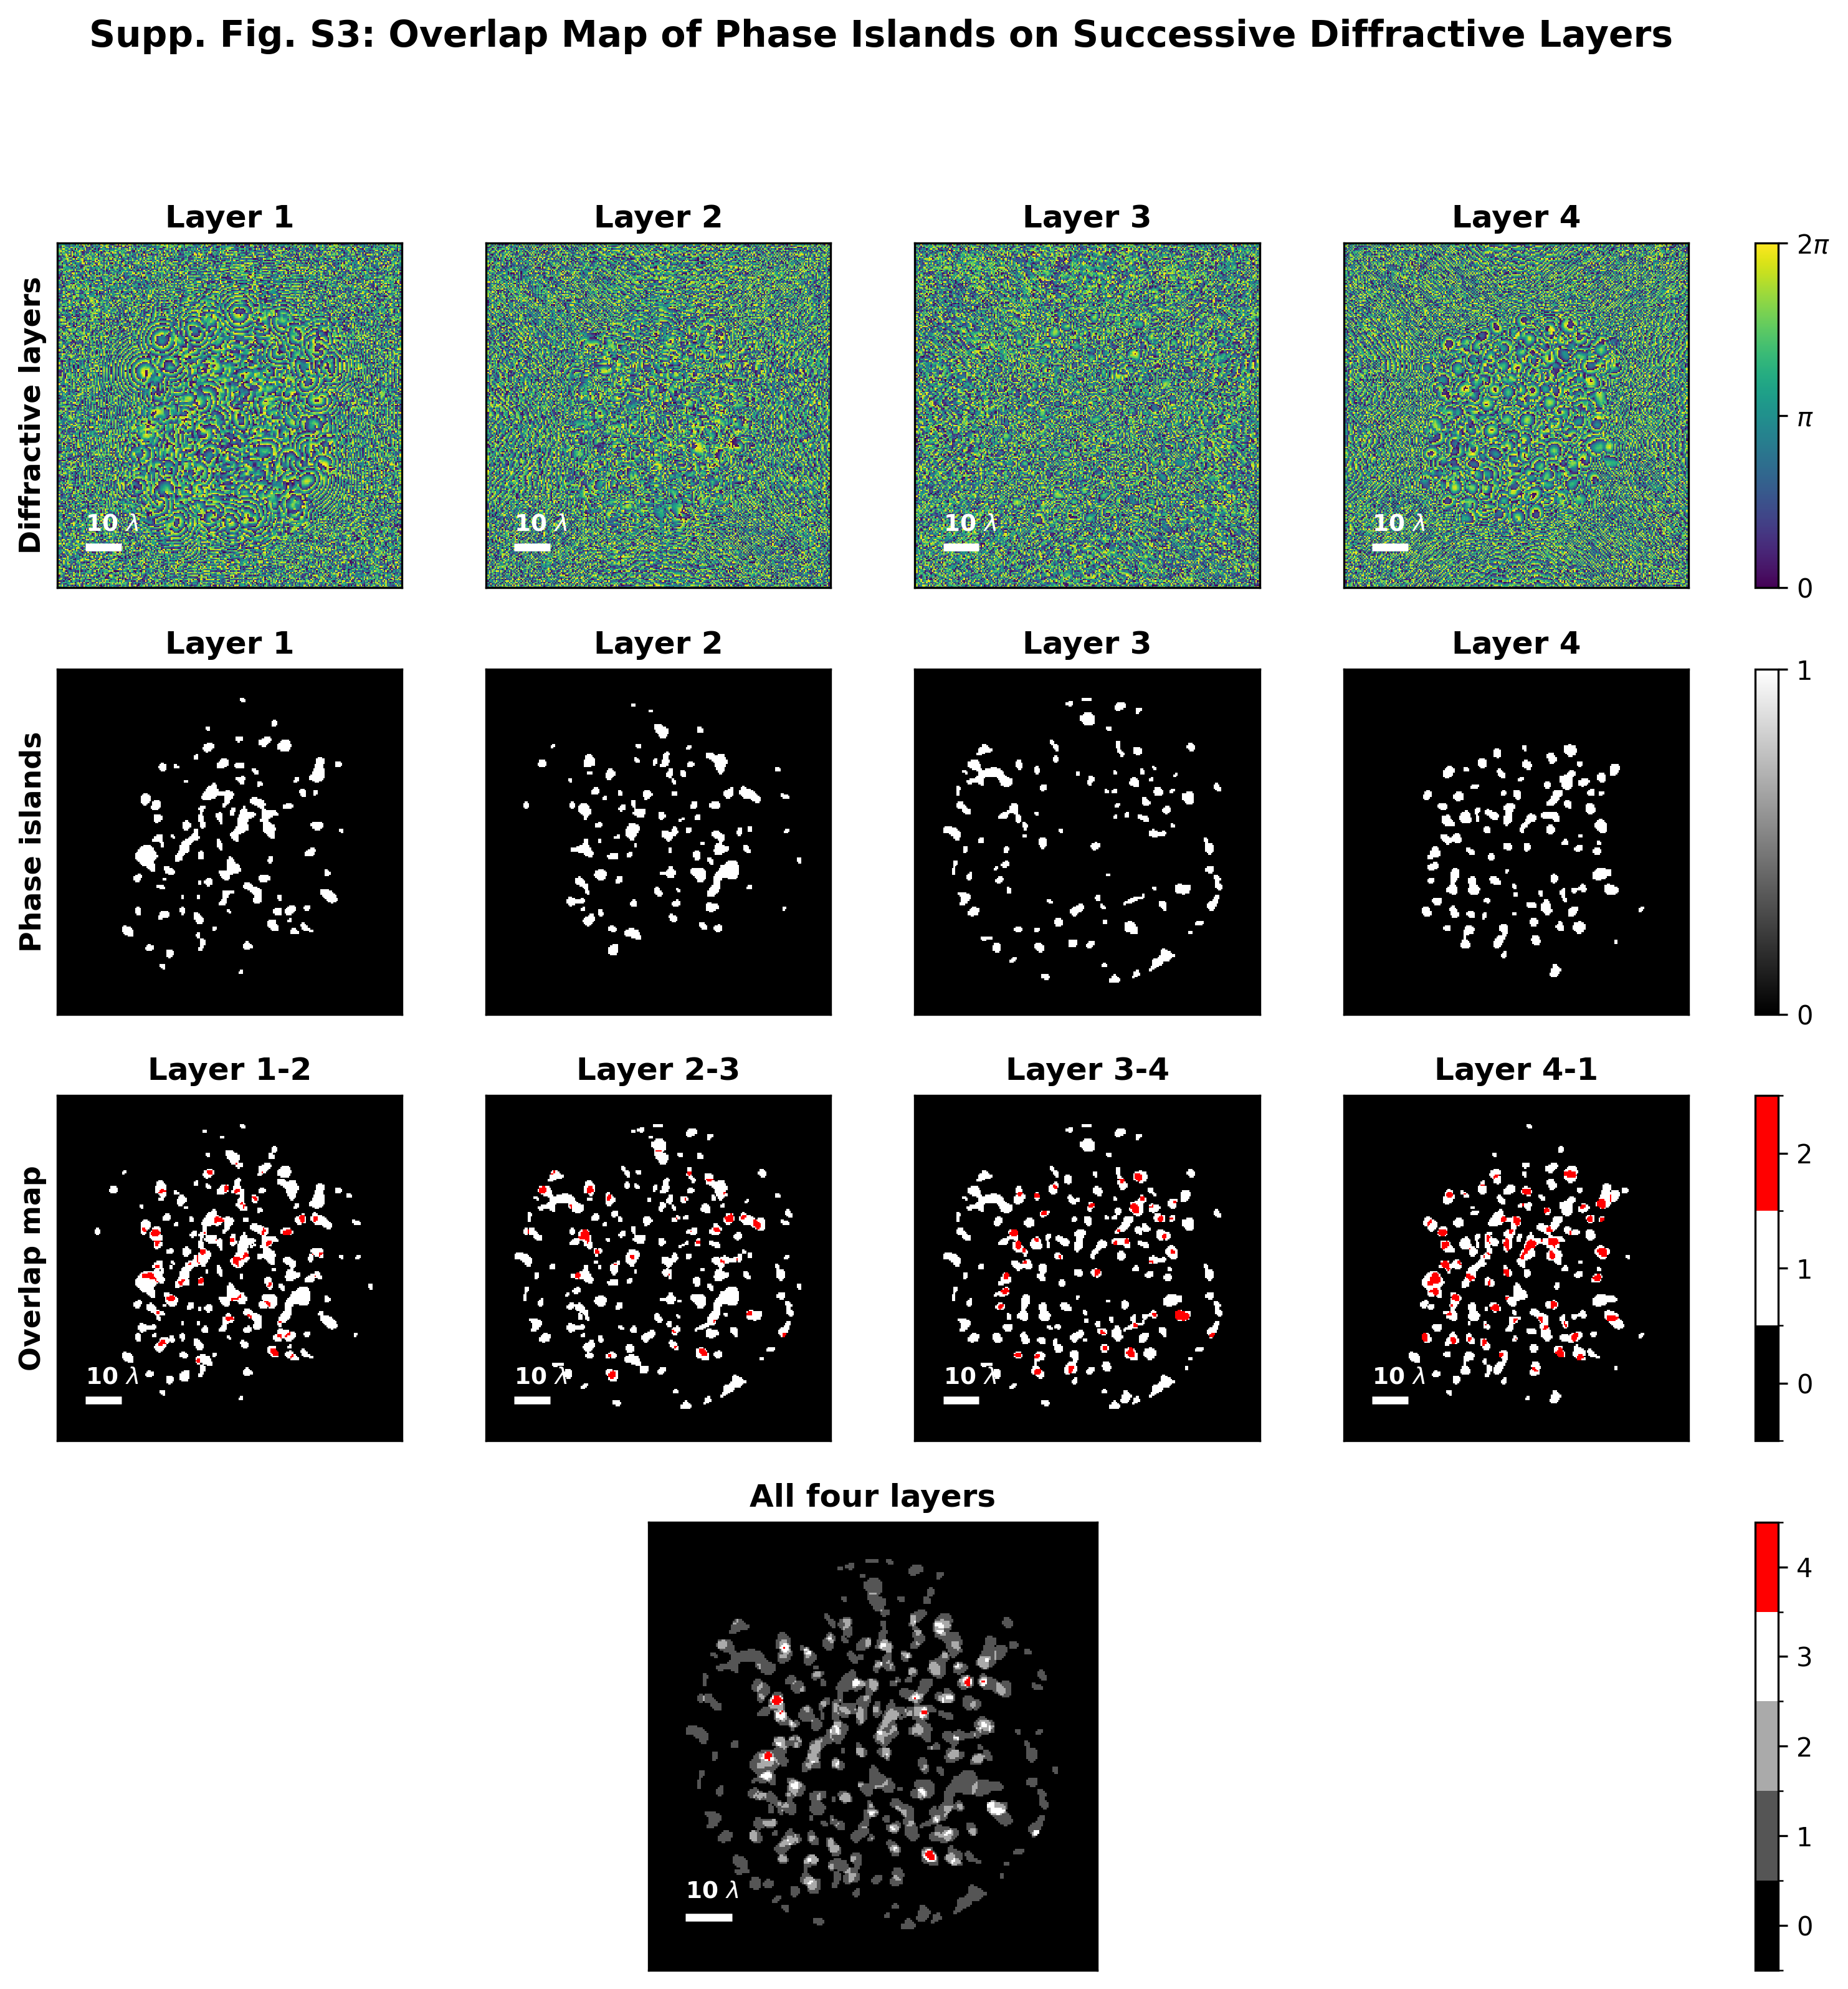
\includegraphics[width=0.85\textwidth]{figS3_overlap_map.png}
  \caption{\textbf{Fig.~S3 재현 --- 위상 섬 중첩 맵}: 4개 레이어의 학습된 위상 패턴에서 추출한 ``위상 섬(phase island)'' 영역의 공간적 분포. 색상 강도가 높을수록 해당 위치에서 더 많은 레이어의 위상 섬이 겹친다. 위상 섬은 그리드 중앙에 집중되는 경향을 보이며, 이는 MNIST 활성 영역(160$\times$160 중앙)과 정확히 대응한다. 주변부의 낮은 중첩도는 해당 영역의 위상을 단순화해도 성능 저하가 제한적임을 시사하며, 이는 TK-26 프루닝 실험의 물리적 근거가 된다.}
  \label{fig:figS3}
\end{figure}

\begin{figure}[H]
  \centering
  \includegraphics[width=0.95\textwidth]{figS4_pruning.png}
  \caption{\textbf{Fig.~S4 재현 --- 프루닝 조건별 성능 비교}: 6가지 마스킹 조건에서의 PCC. \texttt{full\_layers}(마스크 없음)가 baseline이며, \texttt{no\_layers}(위상 레이어 제거)에서 PCC가 급락한다. 주목할 점은 \texttt{islands\_only}(위상 섬만 유지)에서도 baseline의 $\sim$85--90\%의 PCC를 유지한다는 것이다. 이는 학습된 위상 패턴의 핵심 정보가 전체 면적의 10--20\%에 불과한 위상 섬에 집중되어 있으며, 실제 제작 시 이 영역만 정밀하게 제작하고 나머지는 평탄면으로 대체할 수 있는 \textbf{실용적 경로}를 제시한다.}
  \label{fig:figS4}
\end{figure}

\begin{figure}[H]
  \centering
  \includegraphics[width=0.85\textwidth]{figS4_pruning_cli.png}
  \caption{\textbf{Fig.~S4 CLI 재현}: 명령줄 인터페이스를 통한 프루닝 실험 결과. 6단계 조건의 체계적 비교를 보여준다.}
  \label{fig:figS4_cli}
\end{figure}

\subsection{논문의 모호한 서술과 실제 구현 (TK-24\,\textasciitilde\,TK-30)}

\begin{tkbox}[TK-24. ``$n$ diffusers''의 이중 의미]
Training의 $n$(다양성)과 Evaluation의 blind diffuser 수(통계적 신뢰도)는 독립.
\end{tkbox}

\begin{tkbox}[TK-25. Resolution target은 OOD]
3-bar grating은 학습 데이터에 전혀 포함되지 않음. Fig.~3의 핵심: ``산란 보정 자체''의 일반화.
\end{tkbox}

\begin{tkbox}[TK-26. Pruning의 6단계 조건]
\texttt{full\_layers}, \texttt{no\_layers}, \texttt{islands\_only}, \texttt{dilated\_islands}, \texttt{inside\_contour}, \texttt{aperture\_80$\lambda$}. \texttt{no\_layers}는 레이어 자체를 물리적으로 제거.
\end{tkbox}

\begin{tkbox}[TK-27. Phase parameterization]
Raw 값은 $10\pi$ 이상 가능. 분석 시 반드시 \texttt{phase \% (2$\pi$)} wrapping 필요.
\end{tkbox}

\begin{tkbox}[TK-28. 3단계 Resize: 28 $\to$ 160 $\to$ 240 $\to$ 480]
PCC 계산과 display는 중앙 $160 \times 160$에서만 수행. Crop 생략 시 PCC $\sim$0.05 하락.
\end{tkbox}

\begin{tkbox}[TK-29. Blind 시드 분리]
Blind 평가 시드 \texttt{77777777 + i}가 training 시드와 겹치지 않아야 함.
\end{tkbox}

\begin{tkbox}[TK-30. Correlation length 변경: sigma만 변경]
$L \approx 5\lambda$를 위해 \texttt{smoothing\_sigma\_lambda=2.0} 사용. $\Delta n$ 변경 불가.
\end{tkbox}

\subsection{암묵지 의존도 매핑}

\begin{table}[H]
\centering
\caption{주요 암묵지 항목이 영향을 미치는 재현 결과물. $\bullet$ = 직접 영향.}
\label{tab:tkmap}
\small
\begin{tabular}{l ccccc}
\toprule
\thead{암묵지} & \thead{Fig.~2} & \thead{Fig.~3} & \thead{Fig.~S4} & \thead{Fig.~S5} & \thead{Training} \\
\midrule
TK-1--5 (물리+패딩)  & $\bullet$ & $\bullet$ & $\bullet$ & $\bullet$ & $\bullet$ \\
TK-10--13 (학습)      &           &           &           &           & $\bullet$ \\
TK-16 (Height 통계)   & $\bullet$ & $\bullet$ & $\bullet$ & $\bullet$ & $\bullet$ \\
TK-22 (Contrast)      & $\bullet$ &           & $\bullet$ & $\bullet$ &           \\
TK-23 (Amplitude)     & $\bullet$ & $\bullet$ & $\bullet$ & $\bullet$ & $\bullet$ \\
TK-28 (Resize 3단계)  & $\bullet$ & $\bullet$ & $\bullet$ & $\bullet$ & $\bullet$ \\
\bottomrule
\end{tabular}
\end{table}


% ============================================================
% SECTION 7 — 응용 전략
% ============================================================

\section{응용 전략 및 확장 방향}\label{sec:applications}

\begin{insightbox}[Abstract]
$\Delta n = 0.74$의 재료 실현 가능성, THz 대역의 실용 특성, 보안/의료/통신/산업 응용, 스케일링 방향, 그리고 산업화 로드맵을 논의한다.
\end{insightbox}

\subsection{재료 실현 가능성}

\textbf{고분자 기반}: HDPE ($n \approx 1.53$)와 공기의 조합으로 $\Delta n \approx 0.53$. $\Delta n = 0.74$에는 고굴절률 충전재 혼합 또는 TOPAS 기반 복합 구조 필요. THz 대역의 장점은 파장이 길어($\lambda = 750\;\mu\text{m}$) 밀리미터 스케일 3D 프린팅으로 제작 가능하다는 점이다.

\textbf{메타물질 기반}: 실리콘 기반 메타표면은 THz에서 $n_\text{eff} = 1.0$--$3.5$ 범위를 커버할 수 있어 $\Delta n = 0.74$는 용이하게 구현된다.

\subsection{위상판 제작 정밀도}

\begin{table}[H]
\centering
\caption{D2NN 위상 레이어 제작 요구사항.}
\label{tab:fab}
\begin{tabular}{l r l}
\toprule
\thead{파라미터} & \thead{값} & \thead{제작 의미} \\
\midrule
그리드 크기 & $72 \times 72\;\text{mm}^2$ & 표준 THz 마운트 적합 \\
픽셀 피치   & 300\,$\mu$m                 & CNC 밀링 / 3D 프린팅 가능 \\
위상 범위   & $[0, 2\pi)$                 & 최대 높이 $\sim$1.01\,mm \\
위상 정밀도 & $< \pi/10$                  & 높이 정밀도 $\sim$50\,$\mu$m \\
\bottomrule
\end{tabular}
\end{table}

프루닝 분석(Fig.~S4)에서 학습된 위상판의 에너지가 소수의 ``위상 섬(phase island)'' 영역에 집중됨을 발견하였다. 이는 \textbf{핵심 영역만 정밀 제작하고 나머지는 평탄면으로 대체}할 수 있음을 시사한다.

\begin{figure}[H]
  \centering
  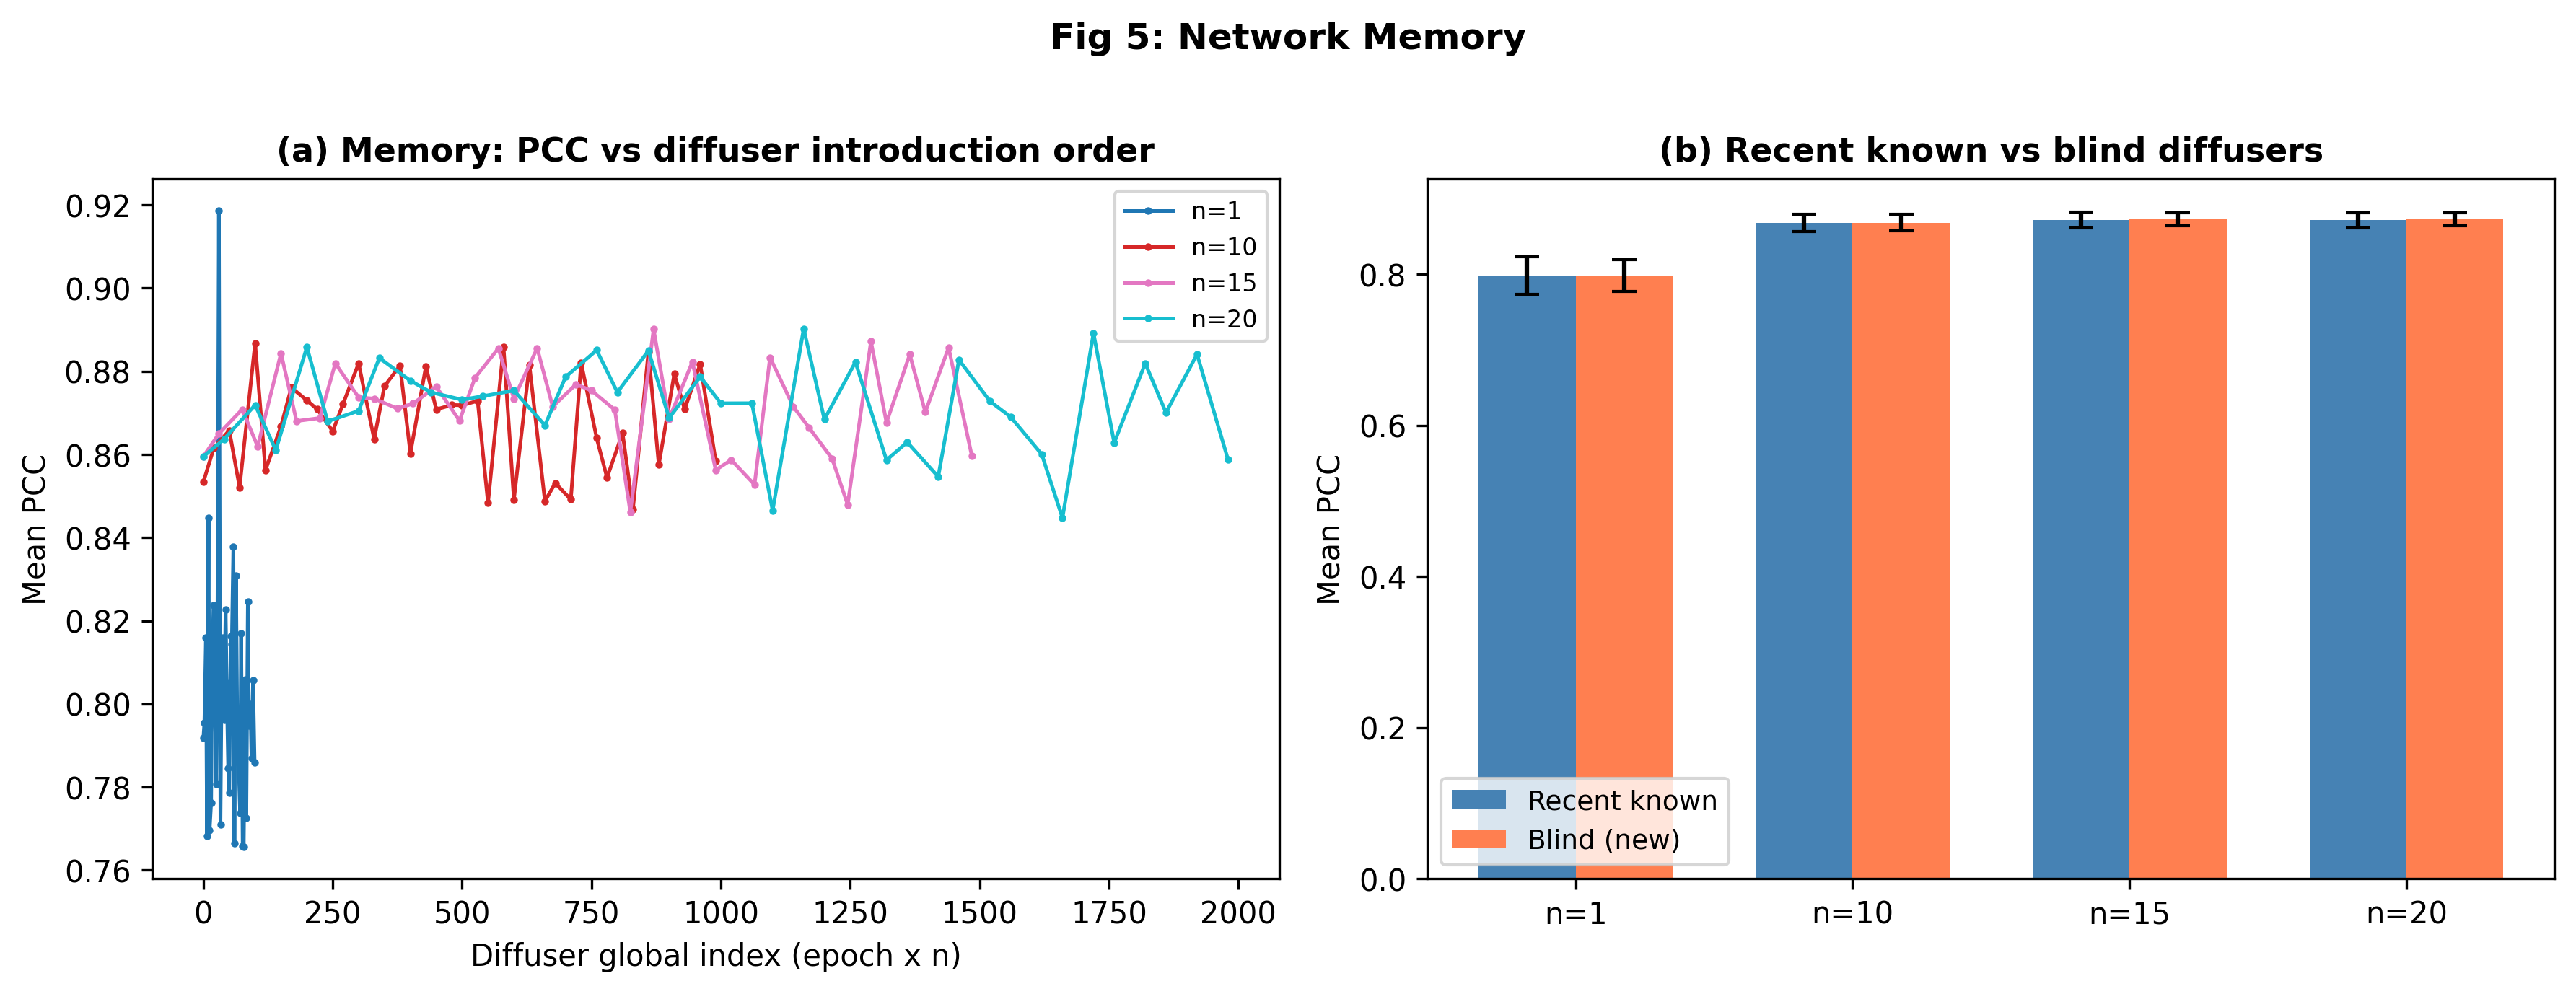
\includegraphics[width=0.85\textwidth]{fig5_memory.png}
  \caption{\textbf{Fig.~5 --- 메모리 분석}: 학습 과정에서의 GPU 메모리 사용량과 $n$ 값의 관계. $B \times n$ 전략에 따라 유효 배치 크기가 선형 증가하며, $n = 20$, $B = 4$에서 $B_\text{eff} = 80$으로 A100 단일 GPU의 실용적 상한에 도달한다. 이 그래프는 ``$n$을 늘리는 비용''을 정량적으로 보여주며, $n = 15$가 Pareto 최적점인 이유의 계산적 근거를 제공한다.}
  \label{fig:fig5}
\end{figure}

\begin{figure}[H]
  \centering
  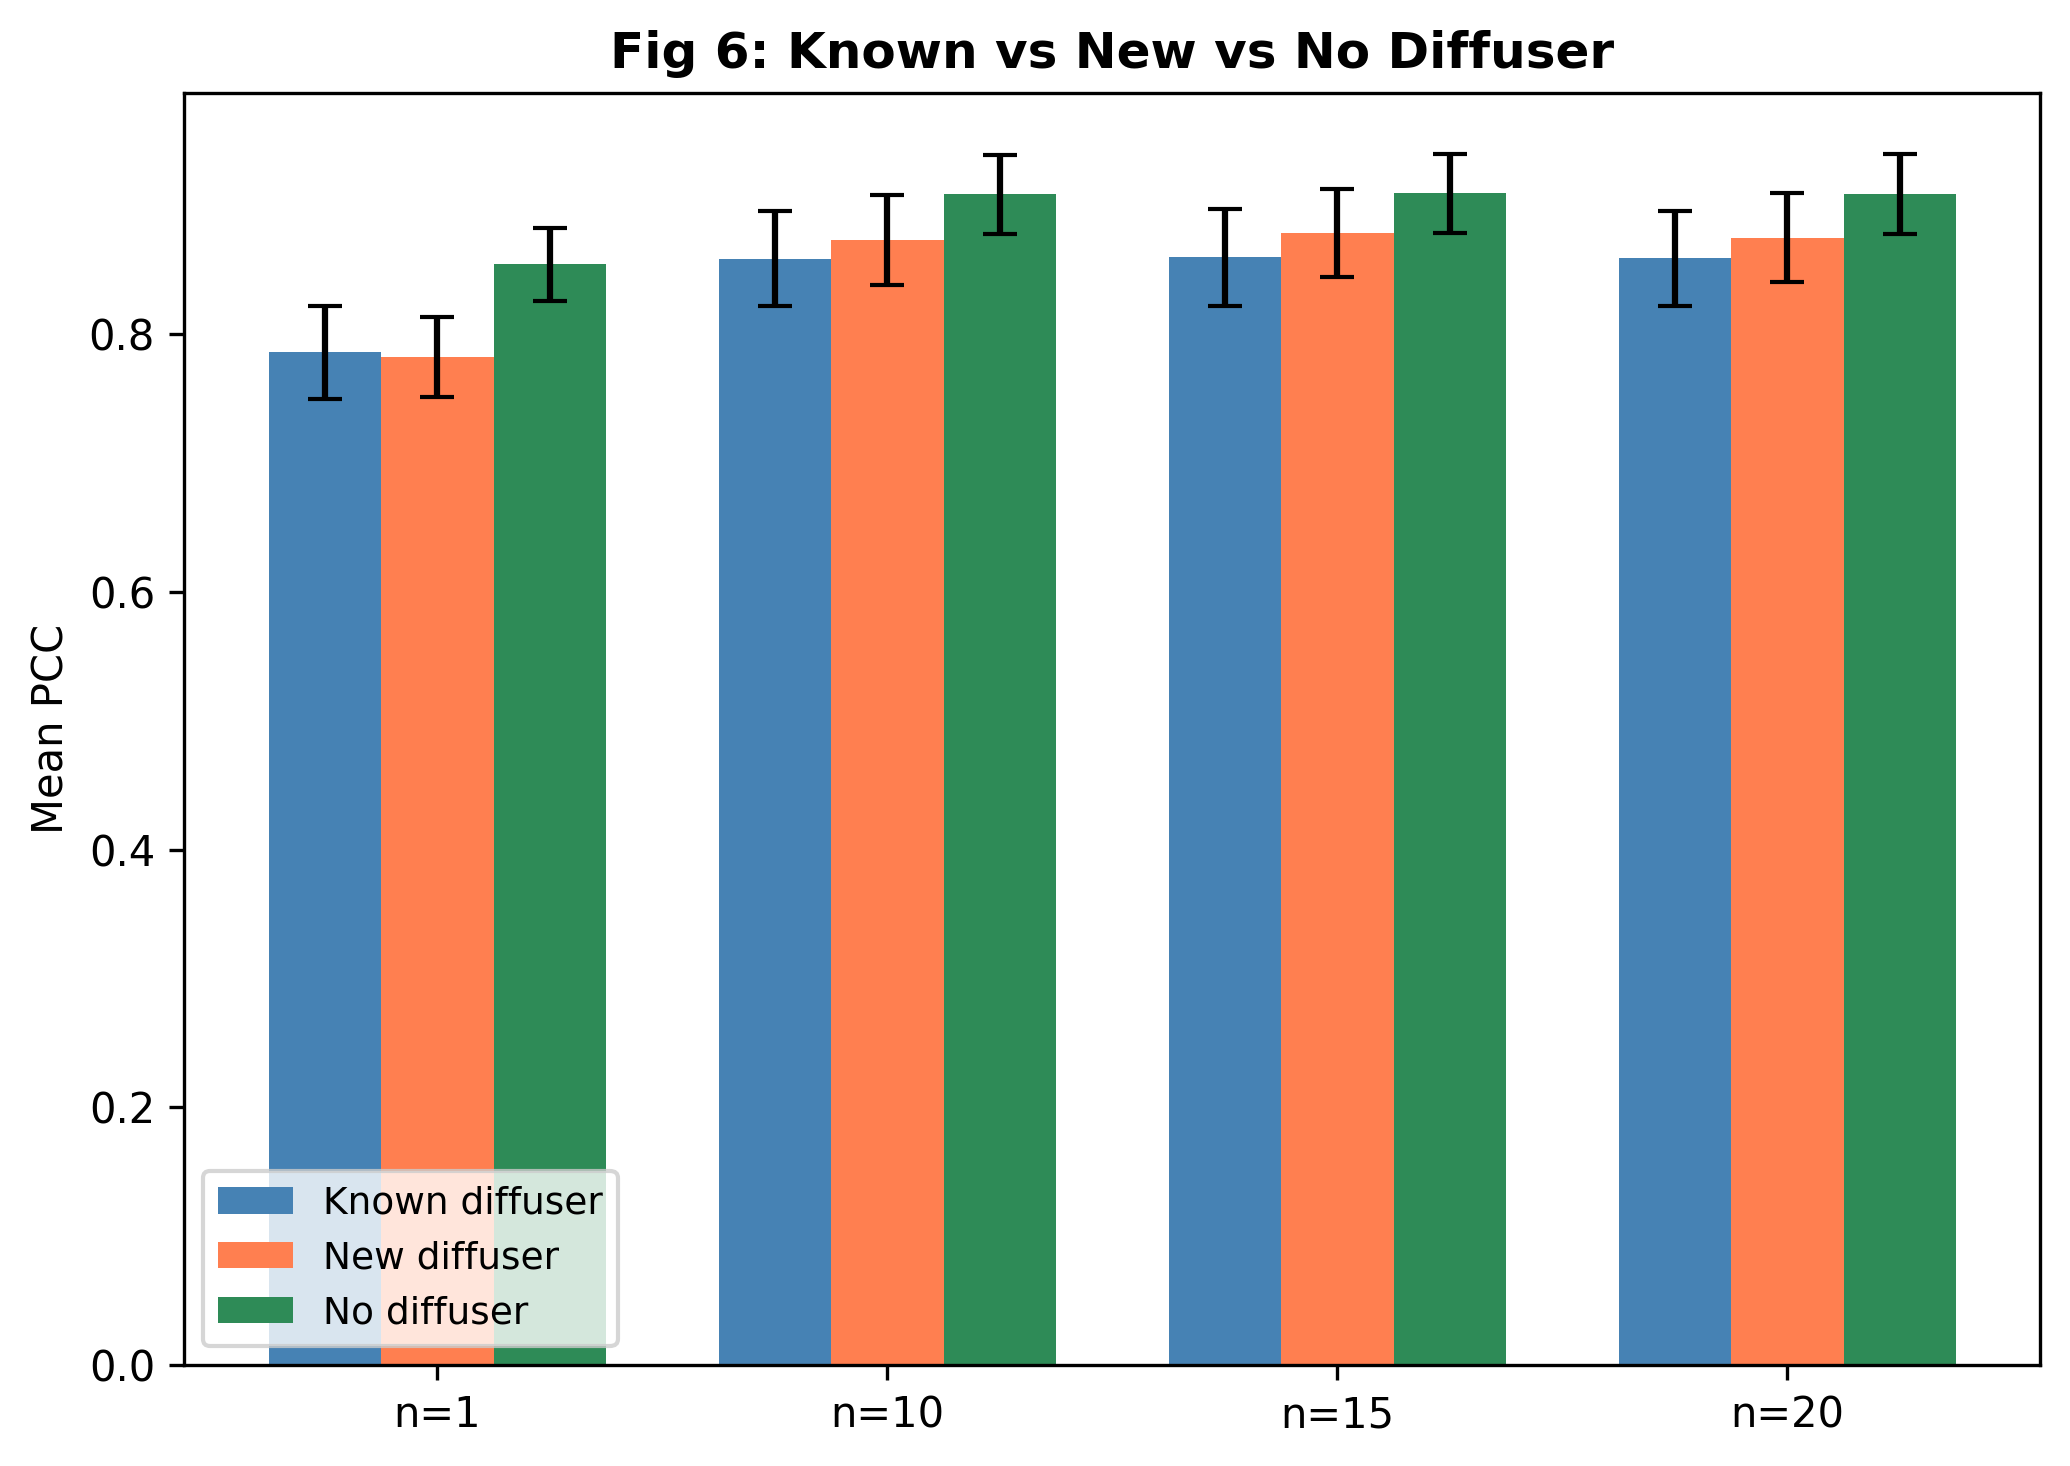
\includegraphics[width=0.95\textwidth]{fig6_conditions.png}
  \caption{\textbf{Fig.~6 --- 실험 조건 총괄}: 4가지 $n$ 값($n = 1, 10, 15, 20$)에 대한 학습 조건과 성능 지표를 비교한 종합 다이어그램. 학습 시간은 $n$에 비례하여 증가하지만, blind PCC 개선은 $n = 15$ 이후 포화한다. 이 비대칭이 ``비용 효율이 중요하면 $n = 15$, 결론의 강도가 중요하면 $n = 20$'' 이라는 실용적 가이드라인의 근거이다.}
  \label{fig:fig6}
\end{figure}

\subsection{구체적 응용 시나리오}

\begin{itemize}
  \item \textbf{보안 영상}: 디퓨저를 PUF(Physical Unclonable Function)로 사용한 물리적 인증 시스템
  \item \textbf{의료 영상}: 피부 아래 조직의 비침습 실시간 영상화, 수분 분포 매핑
  \item \textbf{통신}: 다중 경로 산란의 전광학적 이퀄라이저(equalizer)
  \item \textbf{산업 검사}: 비금속 포장재 투과 THz 검사
\end{itemize}

\subsection{파장대 확장}

\begin{table}[H]
\centering
\caption{파장대별 D2NN 제작 난이도 비교.}
\label{tab:wavelength}
\begin{tabular}{l r r l c}
\toprule
\thead{파장대} & \thead{$\lambda$} & \thead{피치 요구} & \thead{제작 기술} & \thead{난이도} \\
\midrule
THz (현재) & 750\,$\mu$m   & 300\,$\mu$m    & 3D 프린팅, CNC      & 낮음 \\
Far-IR     & 10--30\,$\mu$m & 5--15\,$\mu$m  & 포토리소그래피      & 중간 \\
Mid-IR     & 3--5\,$\mu$m   & 1--2\,$\mu$m   & 반도체 공정         & 높음 \\
Near-IR    & 1--1.5\,$\mu$m & 0.5--0.7\,$\mu$m & 나노임프린트      & 매우 높음 \\
가시광     & 0.4--0.7\,$\mu$m & 0.2--0.35\,$\mu$m & E-beam 리소그래피 & 극히 높음 \\
\bottomrule
\end{tabular}
\end{table}

\subsection{산업화 로드맵}

\textbf{1단계 (TRL 3--4)}: 시뮬레이션 검증 위상 패턴의 3D 프린팅 제작 + 벤치탑 실험 + sim-to-real gap 정량화.

\textbf{2단계 (TRL 5--6)}: 위상 섬 기반 간소화 설계 적용 + 다중 디퓨저 환경 실시간 영상 복원 데모.

\textbf{3단계 (TRL 7--9)}: 사출 성형 대량 생산 + 환경 변동 강건성 검증 + 시스템 소형화·통합 패키징.

\begin{figure}[H]
  \centering
  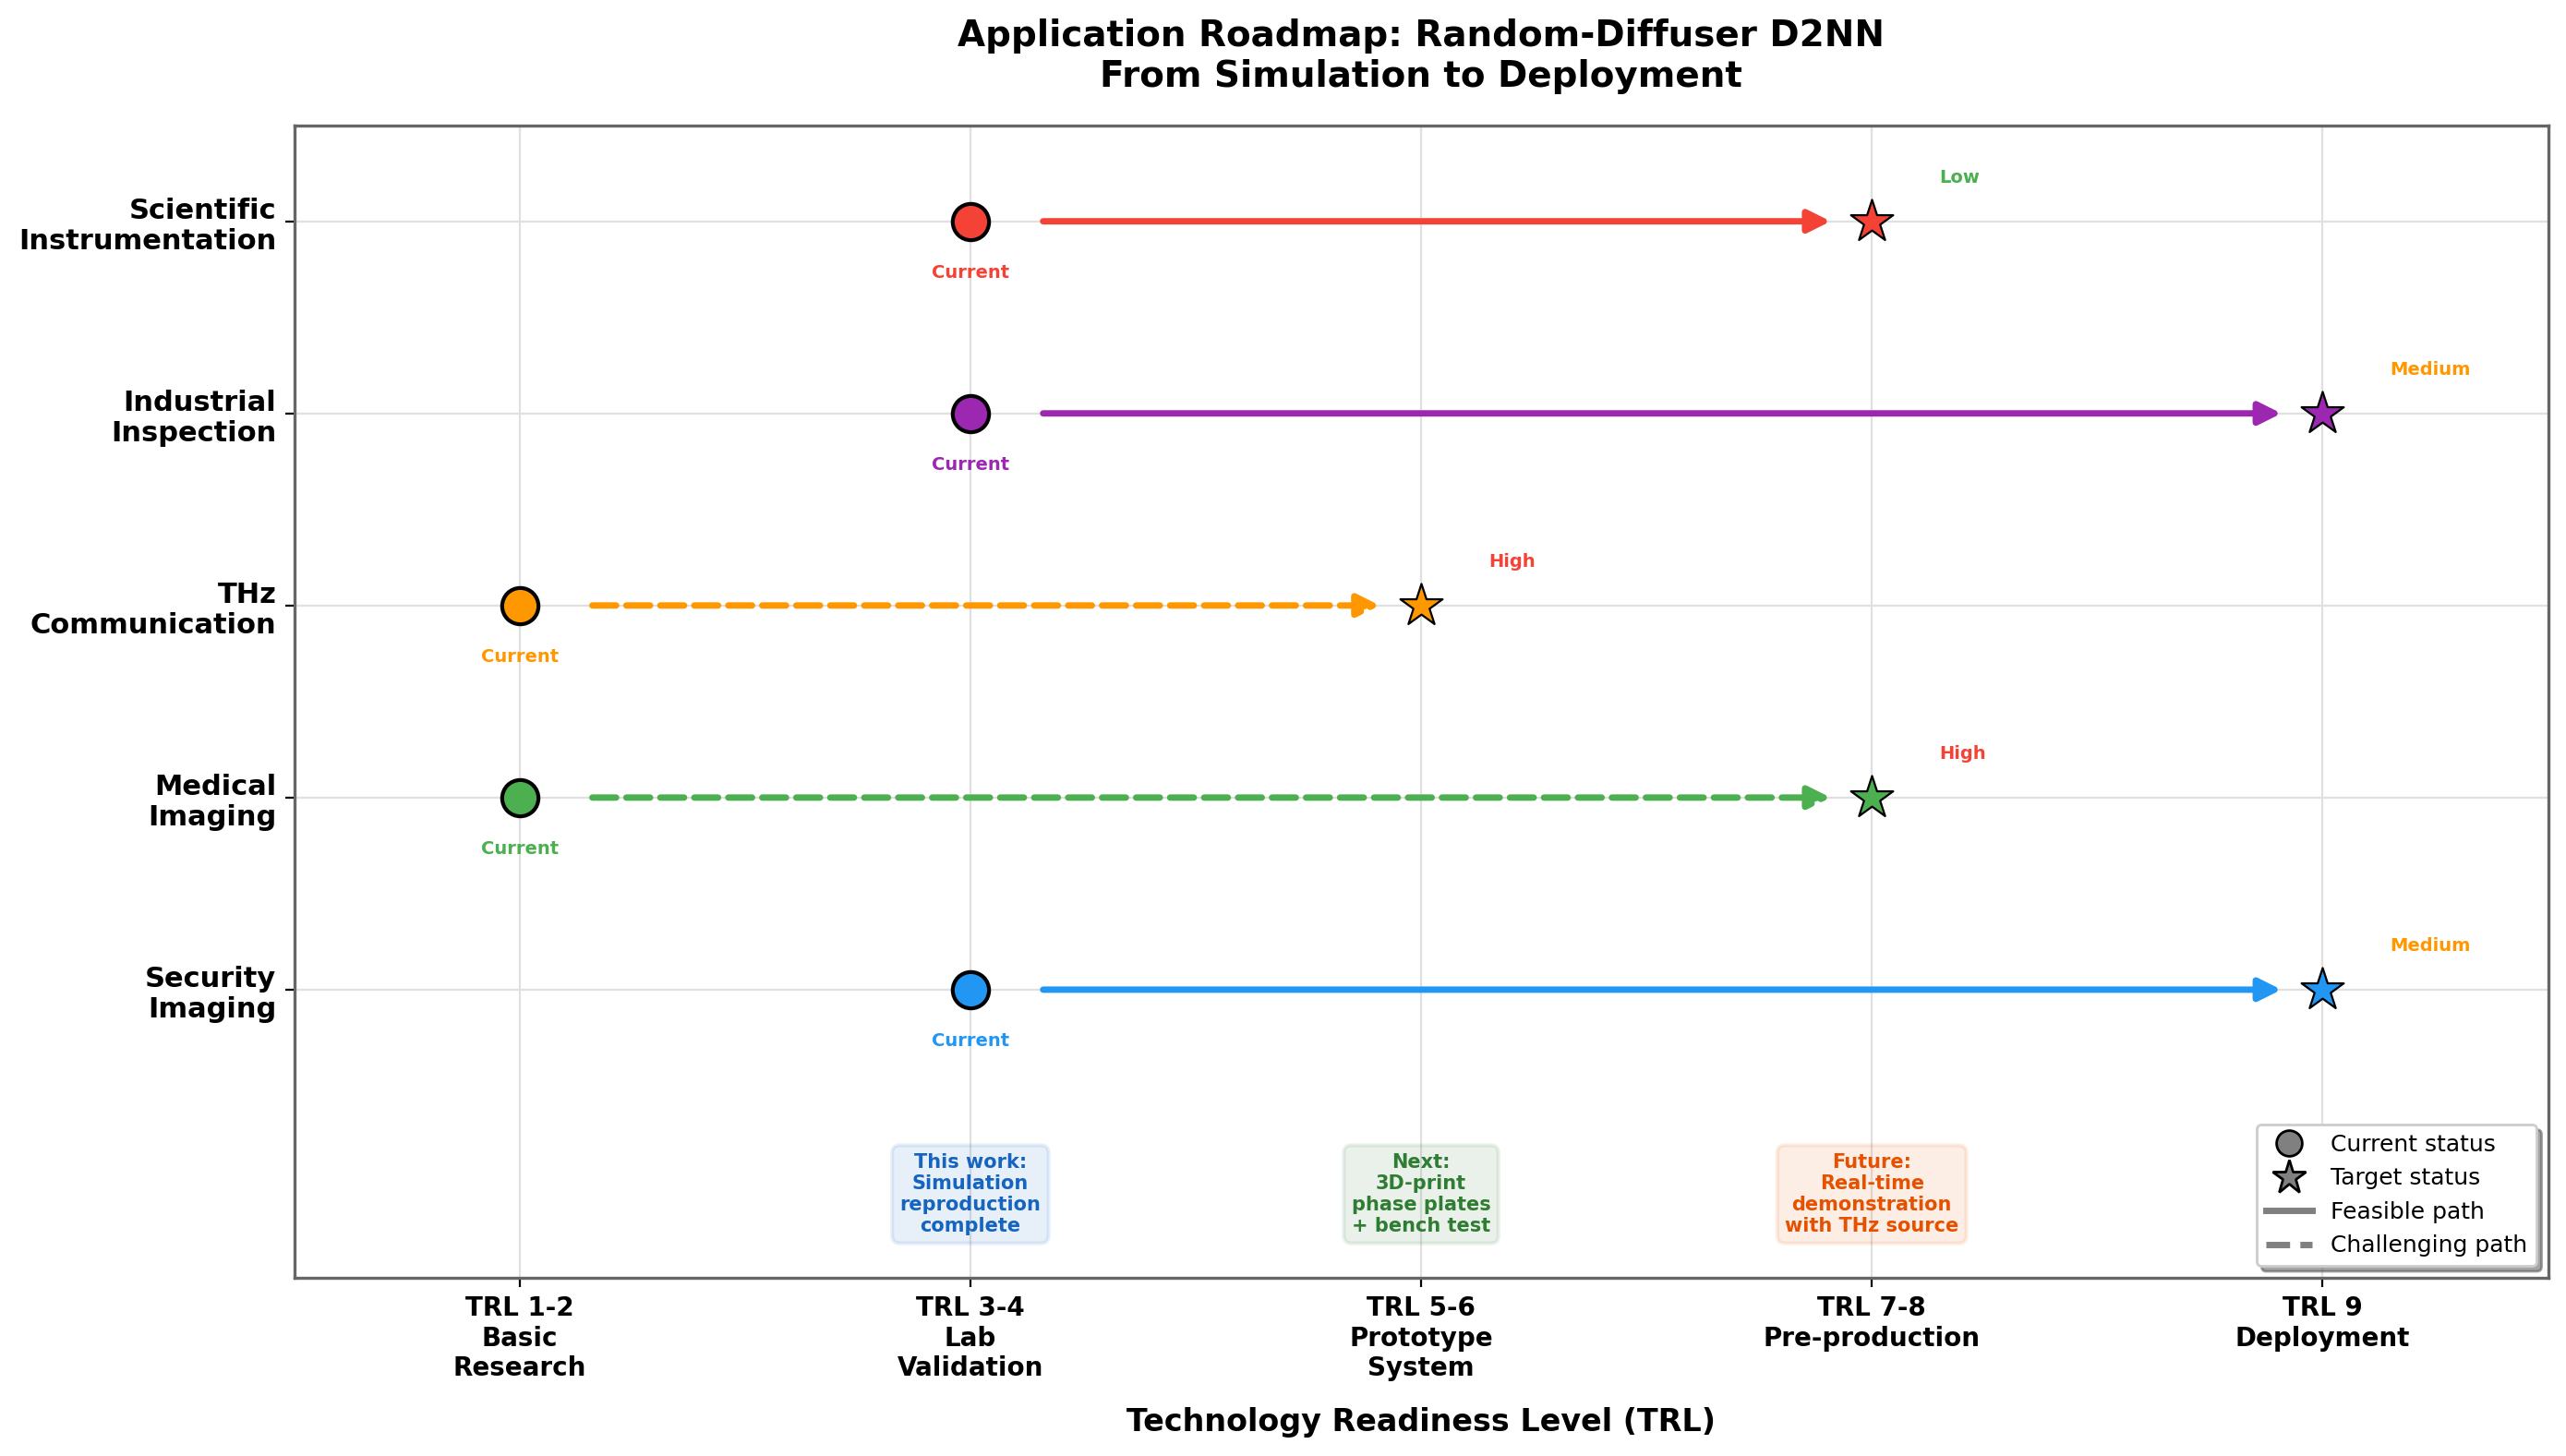
\includegraphics[width=0.85\textwidth]{fig_application_roadmap.png}
  \caption{응용 도메인별 기술 준비도(Technology Readiness Level) 로드맵.}
  \label{fig:roadmap}
\end{figure}

\subsection{제한사항과 극복 방안}

\begin{itemize}
  \item \textbf{스칼라 근사}: 벡터 회절 이론 도입 또는 편광 다양성 학습
  \item \textbf{단일 주파수}: 아크로매틱 메타표면 설계 원리 통합
  \item \textbf{얇은 디퓨저}: 다중 슬라이스(multi-slice) 체적 산란 모델
  \item \textbf{정적 추론}: 재구성 가능한 SLM(Spatial Light Modulator) 사용
\end{itemize}


% ============================================================
% SECTION 8 — 결론
% ============================================================

\section{결론}\label{sec:conclusion}

\subsection{재현 프로젝트의 주요 성과}

\begin{resultbox}[4대 핵심 성과]
\begin{enumerate}
  \item \textbf{$n$-sweep 포화 패턴}: Training PCC $0.907 \to 0.884 \to 0.879 \to 0.878$로 $n \geq 15$에서 명확한 포화
  \item \textbf{일반화 성능}: Blind PCC가 $n = 15$에서 0.872 수준 도달; ``Known $<$ New'' 역전은 distribution-level learning의 증거
  \item \textbf{격자 주기 분해능}: 7.2--12.0\,mm에서 known 및 blind 디퓨저 모두 정확히 복원
  \item \textbf{보충 분석}: 위상 섬(Fig.~S3), 프루닝(Fig.~S4), 상관길이(Fig.~S5) 독립 수행
\end{enumerate}
\end{resultbox}

\subsection{암묵지의 의의}

재현 과정에서 발굴된 30개의 암묵지는 단순한 구현 세부사항이 아니라, D2NN의 물리적 작동 원리를 이해하는 핵심 통찰을 담고 있다:

\begin{itemize}
  \item \textbf{디퓨저 상관길이 $\approx 10\lambda$}: 산란의 각도 분포를 결정하며, D2NN의 수치 개구와 매칭되는 균형점
  \item \textbf{$n = 15$가 Pareto knee}: 계산 비용 대비 일반화 이득의 최적 균형점. 후속 연구는 아키텍처 확장에 우선순위를 두어야 함
  \item \textbf{위상 섬의 집중성}: D2NN이 특정 공간주파수 채널을 선택적으로 활용 $\to$ 제작 간소화와 결함 내성의 물리적 근거
\end{itemize}

\subsection{향후 연구 방향}

\begin{enumerate}
  \item \textbf{깊이 스윕}: $n = 20$ 고정, 레이어 수 2, 4, 6, 8 변화 $\to$ 모델 용량 vs 일반화 분리
  \item \textbf{체적 산란 모델}: 다중 슬라이스 체적 산란체로 현실적 환경 확장
  \item \textbf{실험적 검증}: 학습된 위상 패턴의 3D 프린팅 제작 및 sim-to-real gap 정량화
  \item \textbf{파장대 확장}: THz $\to$ mid-IR $\to$ near-IR로 응용 범위 확장
\end{enumerate}

\vspace{1.5em}

\begin{insightbox}[결어]
본 재현 프로젝트는 Luo et al.\ 2022의 결과가 재현 가능하며(reproducible), 그 핵심 물리적 메커니즘이 견고함(robust)을 확인하였다. 30개의 암묵지를 체계적으로 문서화함으로써, 후속 연구자들이 랜덤 디퓨저 D2NN을 더 효과적으로 확장할 수 있는 토대를 마련하였다. 전광학 컴퓨팅이 실험실 데모를 넘어 실세계 산란 환경으로 나아가는 중요한 이정표이며, 본 보고서가 그 여정에 실질적 기여가 되기를 바란다.
\end{insightbox}

\vfill
\begin{center}
\textcolor{NatGray}{\rule{0.4\textwidth}{0.4pt}}\\[0.5em]
{\small\sffamily\color{NatGray} 본 재현 프로젝트의 전체 코드, 학습된 모델 체크포인트, 원시 데이터는 프로젝트 저장소에 공개되어 있다.}
\end{center}

\end{document}
